\documentclass[11pt,oneside]{article}
\usepackage[a4paper,margin=26mm,headheight=15pt]{geometry}
\usepackage[T1]{fontenc}
\usepackage[utf8]{inputenc}
\IfFileExists{libertinus.sty}{\usepackage{libertinus}}{\usepackage{lmodern}}
\usepackage{microtype}
\usepackage{amsmath,amssymb,amsthm,mathtools,mathrsfs,bm}
% Canonical mathematical notation for active FabiusFunction LaTeX documents.
%
% This file is intentionally a plain TeX input rather than a LaTeX package.
% Every standalone document loads it by an explicit path relative to that
% document's directory; included fragments inherit the definitions from their
% root document.  Keep this file independent of document layout and metadata.
%
% Contract:
%   * one command has one mathematical meaning throughout the active corpus;
%   * names encode semantic roles rather than a document-local choice of letter;
%   * visually similar but differently normalized objects have different print;
%   * every command below is defined normatively in the notation catalogue.
%
% The active corpus excludes docs/archive/.  Historical sources may retain
% their original notation only inside an explicitly labelled quotation.

\makeatletter
\@ifundefined{mathbb}{%
  \PackageError{fabius-notation}{The amssymb package must be loaded first}%
    {Load amsmath and amssymb before inputting fabius-notation.tex.}%
}{}
\@ifundefined{operatorname}{%
  \PackageError{fabius-notation}{The amsmath package must be loaded first}%
    {Load amsmath before inputting fabius-notation.tex.}%
}{}
\makeatother

% Version stamp used by the catalogue and by static audits.
\newcommand{\FabiusNotationVersion}{2026-08-31}

% Number systems.  NaturalNumbers is explicitly the nonnegative convention.
\newcommand{\NaturalNumbers}{\mathbb{N}_{0}}
\newcommand{\PositiveIntegers}{\mathbb{N}_{>0}}
\newcommand{\IntegerNumbers}{\mathbb{Z}}
\newcommand{\RationalNumbers}{\mathbb{Q}}
\newcommand{\RealNumbers}{\mathbb{R}}
\newcommand{\ComplexNumbers}{\mathbb{C}}
\newcommand{\ExtendedRealNumbers}{\overline{\mathbb{R}}}

% The three principal Fabius--Rvachev functions.  Subscripts are deliberate:
% a bare F and a calligraphic F have several unrelated uses in the corpus.
\newcommand{\FabiusBounded}{F_{\mathrm{bd}}}
\newcommand{\FabiusGlobal}{F_{\mathrm{gl}}}
\newcommand{\FabiusQuantile}{Q_{F}}
\newcommand{\FabiusClampedQuantile}{Q_{F,\mathrm{cl}}}
\newcommand{\RvachevUp}{\operatorname{up}}

% Constants, elementary operators, and delimiters.
\newcommand{\EulerE}{\mathrm{e}}
\newcommand{\ImaginaryUnit}{\mathrm{i}}
\newcommand{\Differential}{\mathop{}\!\mathrm{d}}
\newcommand{\AbsoluteValue}[1]{\left\lvert #1\right\rvert}
\newcommand{\Norm}[1]{\left\lVert #1\right\rVert}
\newcommand{\Floor}[1]{\left\lfloor #1\right\rfloor}
\newcommand{\Ceiling}[1]{\left\lceil #1\right\rceil}
\newcommand{\FractionalPart}[1]{\left\{#1\right\}}
\newcommand{\PositivePart}[1]{\left(#1\right)_{+}}
\newcommand{\IndicatorOf}[1]{\mathbf{1}_{#1}}
\newcommand{\SetOf}[1]{\left\{#1\right\}}
\newcommand{\InnerProduct}[1]{\left\langle #1\right\rangle}
\newcommand{\CardinalityOf}[1]{\left\lvert #1\right\rvert}
\newcommand{\DefinitionEquals}{\mathrel{\coloneqq}}
\newcommand{\Sign}{\operatorname{sgn}}
\newcommand{\IdentityOperator}{\operatorname{id}}
\newcommand{\SpanOperator}{\operatorname{span}}
\newcommand{\TraceOperator}{\operatorname{tr}}
\newcommand{\RankOperator}{\operatorname{rank}}
\newcommand{\DiagonalOperator}{\operatorname{diag}}
\newcommand{\ResidueOperator}{\operatorname*{Res}}
\newcommand{\LeastCommonMultiple}{\operatorname{lcm}}
\newcommand{\OrderOperator}{\operatorname{ord}}
\newcommand{\PrincipalLogarithm}{\operatorname{Log}}
\newcommand{\FallingFactorial}[2]{\left(#1\right)^{\underline{#2}}}
\newcommand{\RisingFactorial}[2]{\left(#1\right)^{\overline{#2}}}

% Support, topology, convolution, and metric notation.
\newcommand{\SupportOperator}{\operatorname{supp}}
\newcommand{\SupportOf}[1]{\SupportOperator\!\left(#1\right)}
\newcommand{\TopologicalSupportOf}[1]{\operatorname{tsupp}\!\left(#1\right)}
\newcommand{\Convolution}{\mathbin{*}}
\newcommand{\MetricDistance}{\operatorname{dist}}
\newcommand{\TotalVariationDistance}{d_{\mathrm{TV}}}

% Probability.  Equality and convergence in law are not metric distance.
\newcommand{\Probability}{\mathbb{P}}
\newcommand{\Expectation}{\mathbb{E}}
\newcommand{\Variance}{\operatorname{Var}}
\newcommand{\Covariance}{\operatorname{Cov}}
\newcommand{\LawOperator}{\operatorname{Law}}
\newcommand{\LawOf}[1]{\LawOperator\!\left(#1\right)}
\newcommand{\EqualInLaw}{\mathrel{\overset{\mathrm{law}}{=}}}
\newcommand{\ConvergesInLaw}{\mathrel{\xrightarrow{\mathrm{law}}}}

% Fourier and integral transforms.  The printed labels expose normalization.
% FourierTwoPi uses exp(-2*pi*i*x*xi); FourierAngular uses exp(-i*x*omega).
\newcommand{\FourierTwoPi}[1]{\widehat{#1}_{\,2\pi}}
\newcommand{\FourierAngular}[1]{\widehat{#1}_{\,\mathrm{ang}}}
\newcommand{\LaplaceTransformSymbol}{\mathcal{L}}
\newcommand{\MellinTransformSymbol}{\mathcal{M}}
\newcommand{\LaplaceTransformOf}[1]{\LaplaceTransformSymbol\!\left[#1\right]}
\newcommand{\MellinTransformOf}[1]{\MellinTransformSymbol\!\left[#1\right]}
\newcommand{\MomentGeneratingFunction}[1]{M_{#1}}
\newcommand{\CharacteristicFunction}[1]{\varphi_{#1}}

% The two standard sinc functions must never share one symbol.
\newcommand{\SincRad}{\operatorname{sinc}_{\mathrm{rad}}}
\newcommand{\SincPi}{\operatorname{sinc}_{\pi}}

% Binary arithmetic and Thue--Morse notation.
\newcommand{\BinaryDigitSum}{\operatorname{wt}_{2}}
\newcommand{\ThueMorseSignSymbol}{\varepsilon}
\newcommand{\ThueMorseSign}[1]{\varepsilon_{#1}}
\newcommand{\PadicValuation}[1]{\nu_{#1}}
\newcommand{\TwoAdicValuation}{\nu_{2}}

% q-series notation.  Every base is an explicit argument.
\newcommand{\QPochhammer}[3]{\left(#1;#2\right)_{#3}}
\newcommand{\GaussianBinomial}[3]{%
  \genfrac{[}{]}{0pt}{}{#1}{#2}_{#3}%
}
\newcommand{\QInteger}[2]{\left[#1\right]_{#2}}

% Named special functions.
\newcommand{\Polylogarithm}{\operatorname{Li}}
\newcommand{\LambertW}{W}
\newcommand{\GammaFunction}{\Gamma}
\newcommand{\RiemannZeta}{\zeta}

% Asymptotics.  BigO and LittleO are operator tokens for existing formula
% grammar; prefer the At forms so that the limiting regime is printed.
\newcommand{\BigO}{\mathcal{O}}
\newcommand{\LittleO}{o}
\newcommand{\BigOAt}[2]{\mathcal{O}_{#2}\!\left(#1\right)}
\newcommand{\LittleOAt}[2]{o_{#2}\!\left(#1\right)}

\usepackage{booktabs,longtable,array,tabularx,multirow}
\usepackage{graphicx}
\usepackage{caption}
\usepackage{float}
\usepackage{xcolor}
\usepackage{enumitem}
\usepackage{fancyhdr}
\usepackage{titlesec}
\usepackage{listings}
\usepackage{xurl}
\usepackage[hypertexnames=false]{hyperref}
\usepackage[nameinlink,noabbrev]{cleveref}

\graphicspath{
  {assets/companion-evidence/fabius_dyadic_interpolation_report/figures/}
  {assets/companion-evidence/fabius_interpolation_report/figures/}
  {assets/companion-evidence/Fabius_Rvachev_Dyadic_Interpolation_Report/figures/}
  {assets/companion-evidence/geometric_comb_interpolation_report/}
  {assets/companion-evidence/geometric_comb_interpolation_report-3/figures/}
  {assets/companion-evidence/geometric_comb_q_fabius_report/figures/}
}

\definecolor{linkblue}{RGB}{25,75,135}
\definecolor{deepgreen}{RGB}{28,103,76}
\definecolor{shadegray}{RGB}{246,247,249}
\definecolor{rulegray}{RGB}{195,201,208}
\hypersetup{
  colorlinks=true,
  linkcolor=linkblue,
  citecolor=deepgreen,
  urlcolor=linkblue,
  pdftitle={Comb Interpolation and Sampling Frontiers for the Fabius--Rvachev System},
  pdfsubject={Additive and geometric comb interpolation, exact quadrature, q-calculus, and Fabius--Rvachev sampling},
  pdfkeywords={Fabius function, Rvachev up-function, additive comb, geometric comb, q-binomial, Jackson derivative, Thue-Morse, Euler-Maclaurin, Lagrange interpolation, Richardson extrapolation}
}

\pagestyle{fancy}
\fancyhf{}
\fancyhead[L]{\small Comb-interpolation frontiers}
\fancyhead[R]{\small\nouppercase{\leftmark}}
\fancyfoot[C]{\thepage}
\renewcommand{\headrulewidth}{0.4pt}
\titleformat{\section}{\Large\bfseries}{\thesection}{0.7em}{}
\titleformat{\subsection}{\large\bfseries}{\thesubsection}{0.7em}{}
\titleformat{\subsubsection}{\normalsize\bfseries}{\thesubsubsection}{0.7em}{}
\setcounter{secnumdepth}{3}
\setcounter{tocdepth}{2}
\setlist[itemize]{leftmargin=2em,itemsep=0.25em,topsep=0.4em}
\setlist[enumerate]{leftmargin=2.3em,itemsep=0.25em,topsep=0.4em}
\setlength{\emergencystretch}{3em}
\allowdisplaybreaks[2]
\numberwithin{equation}{section}

% ed.: shared-counter environments now use alias counters (aliascnt) so
% cleveref prints each environment's own name; with the plain
% \newtheorem{lemma}[theorem]{Lemma} pattern every \cref rendered as
% "theorem", even for lemmas, corollaries, and remarks.
\usepackage{aliascnt}
\newcommand{\newsharedtheorem}[2]{%
  \newaliascnt{#1}{theorem}%
  \newtheorem{#1}[#1]{#2}%
  \aliascntresetthe{#1}%
}
\newtheorem{theorem}{Theorem}[section]
\newsharedtheorem{proposition}{Proposition}
\newsharedtheorem{lemma}{Lemma}
\newsharedtheorem{corollary}{Corollary}
\newsharedtheorem{identity}{Identity}
\newsharedtheorem{conjecture}{Conjecture}
\newsharedtheorem{problem}{Problem}
\newsharedtheorem{question}{Research question}
\theoremstyle{definition}
\newsharedtheorem{definition}{Definition}
\newsharedtheorem{algorithm}{Algorithm}
\newsharedtheorem{example}{Example}
\newsharedtheorem{observation}{Numerical observation}
\theoremstyle{remark}
\newsharedtheorem{remark}{Remark}
\newsharedtheorem{warning}{Warning}
\crefname{conjecture}{conjecture}{conjectures}
\Crefname{conjecture}{Conjecture}{Conjectures}
\crefname{problem}{problem}{problems}
\Crefname{problem}{Problem}{Problems}
\crefname{question}{research question}{research questions}
\Crefname{question}{Research question}{Research questions}
\crefname{observation}{numerical observation}{numerical observations}
\Crefname{observation}{Numerical observation}{Numerical observations}
\crefname{identity}{identity}{identities}
\Crefname{identity}{Identity}{Identities}
\crefname{algorithm}{algorithm}{algorithms}
\Crefname{algorithm}{Algorithm}{Algorithms}
\crefname{warning}{warning}{warnings}
\Crefname{warning}{Warning}{Warnings}

\newcommand{\eps}{\varepsilon}
\newcommand{\fall}[2]{#1^{\underline{#2}}}
\newcommand{\rise}[2]{#1^{\overline{#2}}}
\newcommand{\stirlingfirst}[2]{\genfrac{[}{]}{0pt}{}{#1}{#2}}
\newcommand{\Dop}{\mathcal D}
\newcommand{\Bell}{Y}
\newcommand{\ThetaTM}{\Theta}
\newcommand{\defect}{\mathcal R}
\newcommand{\Frow}{\mathscr F}
\newcommand{\ClampedDyadicSample}{D^{\mathrm{cl}}}
\newcommand{\Lag}{\mathcal I}
\newcommand{\Leb}{\mathscr L}
\newcommand{\MM}{\mathsf M}
\newcommand{\Hyp}{\mathsf H}
\newcommand{\repo}{\nolinkurl{Analysis/FabiusFunction/docs}}

\newenvironment{statusbox}[1]{%
  \par\smallskip\noindent\begin{center}\begin{minipage}{0.94\textwidth}%
  \hrule\vspace{0.5em}\noindent\textbf{#1}\par\smallskip
}{%
  \vspace{0.5em}\hrule\end{minipage}\end{center}\smallskip
}

\lstdefinestyle{pythonstyle}{
  language=Python,
  basicstyle=\ttfamily\footnotesize,
  backgroundcolor=\color{shadegray},
  frame=single,
  rulecolor=\color{rulegray},
  columns=fullflexible,
  keepspaces=true,
  showstringspaces=false,
  breaklines=true,
  xleftmargin=0.7em,
  xrightmargin=0.7em,
  aboveskip=0.8em,
  belowskip=0.8em
}


\newcommand{\Nzero}{\mathbb N_0}
\newcommand{\halfbinom}[2]{\GaussianBinomial{#1}{#2}{1/2}}
\newcommand{\twobinom}[2]{\GaussianBinomial{#1}{#2}{2}}
\newcommand{\App}{\mathcal A}
\newcommand{\Interp}{\mathcal I}
\newcommand{\GeomLeb}{\Lambda}
\newcommand{\MGF}{\mathcal M}
\newcommand{\PiN}{\Pi}
\newcommand{\Gc}{\mathcal G}
\newcommand{\Rc}{\mathcal R}
\newcommand{\Ic}{\mathcal I}
\newcommand{\Dc}{\mathcal D}
\newcommand{\Cc}{\mathcal C}
\newcommand{\Bc}{\mathcal B}
\newcommand{\Thetaop}{\Theta}
\newcommand{\Mellin}{\mathcal M}
\newcommand{\Gop}{\mathcal G}
\newcommand{\Iop}{\mathcal I}
\newcommand{\Dq}{D_q}
\newcommand{\Mq}{\mathsf M_q}
\newcommand{\qfac}[2]{\left[#1\right]_{#2}!}

\newenvironment{resultbox}
{\par\medskip\noindent\begin{center}\begin{minipage}{0.94\textwidth}\hrule\medskip}
{\medskip\hrule\end{minipage}\end{center}\medskip}


\title{\bfseries Comb Interpolation and Sampling Frontiers\\[0.4em]
\large Additive and geometric combs in the Fabius--Rvachev system}
\author{Consolidated frontier volume for Vladimir Reshetnikov's \texttt{ProveIt} project}
\date{31 August 2026}

\begin{document}
\maketitle
\begin{abstract}
\sloppy
This volume unifies two sampling geometries for the Fabius--Rvachev system.
Its additive dyadic comb yields exact generating functions for each row,
Bell--Prouhet compression, terminating
Euler--Maclaurin formulae, phase-sensitive Rvachev cubature, and sharp global
interpolation instability with stable local alternatives.  On the geometric
comb $cq^{\NaturalNumbers}$ it develops Gaussian-Pascal and Jackson--Newton
calculus, exact residual and stability formulae, Mellin and regular-variation
filters, geometric-knot splines, inverse-dyadic Fabius transforms, and finite
Rvachev synthesis.  The common algebra explains why Gaussian binomials,
Bernoulli and Bell polynomials, Thue--Morse cancellation, Richardson
extrapolation, Lambert $W$, and the Rvachev sinc product repeatedly meet in the
same problem.

The text consolidates four live manuscripts and, through the additive-dyadic
manuscript, nine earlier source packages.  Repeated geometric-comb derivations
are stated once in their strongest form.  Independent extensions are retained
with their own proofs.  Every theorem, proposition, lemma, and corollary in
this volume has an explicit human-readable proof; every unproved mathematical
claim is visibly labelled as a conjecture, problem, or research question.
\end{abstract}

\begin{statusbox}{Proof and evidence terminology}
\textbf{Lean-proved} means that the theorem concordance names an exact compiled
declaration in the repository.  \textbf{Human-proved frontier result} means
that a complete manuscript proof is present here but no exact Lean declaration
has been validated.  \textbf{Conjecture} and \textbf{problem} mean that a
genuine proof obligation remains.  Numerical tables, symbolic checks, and
plots are reproducibility evidence, never proof premises.  A module-level
connection is not reported as a Lean proof unless an exact declaration has
been checked.  When compiled declarations cover only proper subclaims of a
compound manuscript result, the concordance keeps that result at manuscript
status and records the narrower Lean support without upgrading the whole row.
\end{statusbox}

\section*{Editorial scope and reading map}
\addcontentsline{toc}{section}{Editorial scope and reading map}

The geometric-comb part comes first because its affine and multiplicative
algebra supplies the reusable interpolation language.  The strongest source
is used for the finite spine: geometric Newton products, Jackson divided
differences, Gaussian-Pascal basis changes, Lagrange cardinals, complete
homogeneous residuals, and the endpoint/global stability dichotomy.  Two
independent reports then contribute only what is genuinely additional:
confluent Puiseux--log filters, Mellin symbols, regular summability, superflat
divergence, geometric-uniform laws, positive B-spline remainders, and the
reciprocal sinc-product filter.  The later parts return to the additive dyadic
comb for exact quadrature and endpoint-flat interpolation.

The provenance appendix records every source at an immutable Git revision.
The theorem concordance gives a one-to-one disposition for every source result
environment.  The source-disposition and companion-payload ledgers similarly
account for every pre-retirement file.  Git history remains the byte-for-byte
archive; the live tree contains only the canonical publication and the unique
evidence needed to reproduce it.

\subsection*{Normalizations}

Throughout, $0<q<1$ unless a result explicitly says otherwise.  A geometric
comb has nodes $cq^j$; an additive dyadic comb has mesh $2^{-m}$.  The bounded
Fabius distribution function is denoted $F$, and $\RvachevUp$ denotes
Rvachev's compactly supported even up-function.  The shared notation catalogue
imported by the master source governs $q$-Pochhammer symbols, Gaussian
coefficients, expectations, valuations, asymptotic notation, and named number
systems.  Local symbols are introduced once at first use.

\clearpage
\tableofcontents
\clearpage
% Mechanically selected from the pinned gq source; labels use gq:.
\part{Algebra of the geometric comb}

\section{Scope, provenance, and normalization}
\label{gq:chap:scope}

\subsection{Relation to the canonical source and neighboring reports}

The starting point is the forward-theory chapter on negative upper indices
and geometric Newton interpolation in the canonical source
\path{q_pochhammer_q_binomial_monograph.tex}.  That chapter already records the
basic divided-difference formula on $1,q,\ldots,q^n$.  The present report
expands that seed in four directions:

\begin{enumerate}
\item it develops the full change-of-basis and residual algebra, rather than
      treating geometric interpolation as an isolated application;
\item it separates local convergence near the accumulation point from global
      stability on the convex hull and proves sharp asymptotics for both;
\item it specializes the transforms to the inverse-dyadic Fabius data and
      obtains exact boundary-residue and endpoint-jet estimates;
\item it composes the geometric interpolant with the existing Rvachev
      polynomial-synthesis operator, thereby connecting $q$-Pochhammer
      coordinates to finite dictionaries of compactly supported atomic
      functions.
\end{enumerate}

The uniform dyadic-comb report is used only for comparison: its nodes
$j/2^m$ fill $[0,1]$ but suffer the familiar global high-degree instability.
The geometric comb $2^{-j}$ has a different pathology: it samples one
boundary on all binary scales, but it leaves a fixed gap $(1/2,1)$.  The
Rvachev--Lagrange loop report supplies the exact inverse-moment Appell
synthesis of polynomials by translates of $\RvachevUp$.  Results imported from those
reports are identified when used; the report-specific derivations carry
manuscript proofs here.

Results developed here means beyond the explicitly inspected source set at
the pinned repository snapshot; it is neither an exhaustive repository
nonduplication certificate nor a claim of unrestricted world priority.
Classical background
on $q$-series and $q$-calculus is available in
\cite{Andrews1986,GasperRahman2004,KacCheung2002,DLMF17}; the $q$-Newton
viewpoint is particularly explicit in \cite{Kupershmidt2000}.  Barycentric
interpolation and its numerical evaluation are treated in
\cite{BerrutTrefethen2004,Higham2004}.

\subsection{Manuscript proof versus Lean proof}
\label{gq:sec:lean-boundary}

In this document, ``proved'' means proved in the displayed mathematical
argument.  It does not mean that the statement has a corresponding Lean
declaration.  The formal API was audited at the source snapshot
\path{e5175d5eb78d66f4e31db3bc506541b9bae12c57}; the relevant files and
declarations listed below were unchanged when rechecked at intake head
\path{ffcdbdac47246bd553f272bd1ceac441f8dd4f0c}.  The current crosswalk also
audits the later compiled module
\path{FabiusFunction.LagrangeRvachevSynthesis}; that current formal API is
separate from the immutable manuscript source pin.

The repository already formalizes substantial finite foundations:
\begin{enumerate}
\item finite $q$-Pochhammer and Gaussian-binomial algebra, including
      \path{finite_qBinomial_theorem} and
      \path{gaussianBinomial_reciprocity};
\item complete-homogeneous specialization on a geometric alphabet via
      \path{completeHomogeneousEvalOn_geometric_range};
\item geometric evaluation-at-zero weights, all rational power residuals,
      and their exact finite $\ell^1$ norm via
      \path{geometricLagrangeWeight_eq_qBinomial},
      \path{geometricLagrangeQMoment_eq_residual_qBinomial}, and
      \path{sum_abs_geometricLagrangeWeight_eq_qPochhammer_ratio};
\item the inverse-dyadic Fabius moment identity
      \path{halfMoment_eq_fabius_formula};
\item Rvachev moment/Appell deconvolution and global and finite polynomial
      synthesis, in particular
      \path{integral_eval_rvachevDeconvolvedPolynomial_add_mul_rvachev}
      and
      \path{normalized_sum_Ioo_rvachevDeconvolvedPolynomial_mul_shifted_rvachevUp}.
\item generic finite Lagrange--Rvachev synthesis for arbitrary node families:
      \path{normalized_sum_Ioo_lagrangeRvachevDecoder_mul_shifted_rvachevUp},
      \path{normalized_sum_Ioo_lagrangeRvachevDecoder_eval_node},
      \path{lagrangeRvachevAtomCoefficient_eq_deconvolved_interpolate},
      \path{sum_Ioo_lagrangeRvachevAtomCoefficient_mul_shifted_rvachevUp},
      and \path{sum_lagrangeRvachevDecoder_eq_one}.
\end{enumerate}

No one-to-one Lean declaration was found for this report's Jackson
divided-difference theorem, Gaussian Newton basis pair, arbitrary-evaluation
complete-homogeneous interpolation remainder, analytic infinite Newton
convergence theorem, boundary-layer or global Lebesgue asymptotics,
Newton--Jackson quadrature, Fabius boundary-residue and fixed-jet bounds,
gap-growth bound, the closed geometric Gaussian--Appell decoder formula and
prefactor, or the Matrix-level right-inverse/stochastic-encoder package.
The new scalar Lagrange--Rvachev API covers the generic synthesis,
coefficient, nodewise-biorthogonality, and decoder-row-sum layers only.  Some
remaining statements follow on paper from formalized finite ingredients, but
that is not the same as a checked Lean theorem.  The conjectures and research
problems have no proof status in either layer.

\subsection{The affine geometric comb}

\begin{definition}[Affine geometric comb]
Let $\alpha,\beta,q\in\ComplexNumbers$ with $\beta\ne0$.  The degree-$n$ affine geometric
comb is
\[
 \mathcal G_n(\alpha,\beta;q)
 :=\{\alpha+\beta q^j:0\le j\le n\}.
\]
When $|q|<1$, its infinite continuation accumulates at $\alpha$.  The
multiplicative normalization is $\alpha=0$, $\beta=c$; the reflected
boundary normalization used for $\RvachevUp$ is $\alpha=1$, $\beta=-1$.
\end{definition}

Finite interpolation requires distinct nodes, equivalently
$q^d\ne1$ for $1\le d\le n$.  Most algebraic formulae remain valid over an
arbitrary field under that hypothesis.  The convergence and Lebesgue theory
will assume
\begin{equation}
 0<q<1,
 \qquad c>0,
 \qquad x_j=cq^j.
 \label{gq:eq:real-normalization}
\end{equation}
The affine case is recovered by $z=(x-\alpha)/\beta$.

\begin{proposition}[Affine covariance]
Let $P$ interpolate $f$ on $\mathcal G_n(\alpha,\beta;q)$ and set
$g(z)=f(\alpha+\beta z)$.  If $Q$ interpolates $g$ on
$1,q,\ldots,q^n$, then
\[
 P(x)=Q\!\left(\frac{x-\alpha}{\beta}\right).
\]
The Lagrange cardinals transform by the same substitution, and the Lebesgue
function is invariant under real affine changes that map the interpolation
interval bijectively to itself.
\end{proposition}

\begin{proof}
Both sides are polynomials of degree at most $n$ and agree at all $n+1$
nodes.  The cardinal and Lebesgue assertions follow immediately.
\end{proof}

Thus $c$ is retained in algebraic formulae to expose homogeneity, but it can
be set to $1$ in all conditioning arguments.

\subsection{Notation for \texorpdfstring{$q$}{q}-analogues}

For $k\in\NaturalNumbers$,
\begin{align}
 (a;q)_k&:=\prod_{r=0}^{k-1}(1-aq^r),
 & (a;q)_0&:=1,\\
 [k]_q&:=\frac{1-q^k}{1-q},
 & [k]_q!&:=\prod_{r=1}^k[r]_q=\frac{(q;q)_k}{(1-q)^k},\\
 \GaussianBinomial{n}{k}{q}&:=\frac{(q;q)_n}{(q;q)_k(q;q)_{n-k}}
 &&(0\le k\le n).
\end{align}
The Gaussian coefficient is a polynomial in $q$; quotient notation is used
only where the displayed denominators are nonzero.  Reciprocity reads
\begin{equation}
 \GaussianBinomial{n}{k}{q^{-1}}=q^{-k(n-k)}\GaussianBinomial{n}{k}{q}.
 \label{gq:eq:q-reciprocity}
\end{equation}
The complete homogeneous symmetric polynomial is characterized by
\begin{equation}
 \prod_{j=0}^m\frac1{1-y_jt}
 =\sum_{r\ge0}h_r(y_0,\ldots,y_m)t^r.
 \label{gq:eq:h-generating}
\end{equation}
Its geometric principal specialization is
\begin{equation}
 h_r(c,cq,\ldots,cq^m)=c^r\GaussianBinomial{m+r}{m}{q}.
 \label{gq:eq:h-principal}
\end{equation}
This simple identity is the source of almost every Gaussian coefficient in
the residual formulae below.

\section{Newton interpolation as \texorpdfstring{$q$}{q}-Taylor calculus}
\label{gq:chap:q-newton}

\subsection{The \texorpdfstring{$q$}{q}-Pochhammer Newton basis}

\begin{definition}[Geometric Newton polynomial]
For $k\ge0$, define
\begin{equation}
 N_k(x;c,q):=\prod_{r=0}^{k-1}(x-cq^r),
 \qquad N_0:=1.
 \label{gq:eq:newton-basis}
\end{equation}
\end{definition}

The factor locations are exactly the first $k$ nodes of the comb.  Pulling
out $-cq^r$ from each factor gives the fundamental identification
\begin{equation}
 \boxed{
 N_k(x;c,q)=(-c)^kq^{\binom k2}(x/c;q^{-1})_k.}
 \label{gq:eq:newton-pochhammer}
\end{equation}
Thus the finite $q$-Pochhammer symbol is not merely analogous to a Newton
basis: on a geometric grid it \emph{is} the Newton basis, up to its monic
normalization.

Let
\begin{equation}
 (D_qf)(x):=\frac{f(x)-f(qx)}{(1-q)x},
 \qquad x\ne0,
 \label{gq:eq:Dq}
\end{equation}
with the removable value at $0$ used when it exists.  The usual $q$-Leibniz
rule gives
\begin{equation}
 D_qN_k(x;c,q)=[k]_qN_{k-1}(x;c,q).
 \label{gq:eq:Dq-newton}
\end{equation}
A direct proof follows by writing $N_k=(x-c)_{q}^{k}$ in the standard
$q$-falling-power notation.  The next theorem supplies the exact data-side
operator and fixes every power of $q$.

\begin{theorem}[Iterated Jackson difference and geometric divided difference]
\label{gq:thm:Dq-divided-difference}
Let $E_qf(x)=f(qx)$.  For every $k\ge0$,
\begin{align}
 D_q^k
 &=\frac{x^{-k}}{(1-q)^k}(E_q;q^{-1})_k,
 \label{gq:eq:Dq-operator-factor}\\
 D_q^kf(x)
 &=\frac{x^{-k}}{(1-q)^k}
   \sum_{j=0}^k(-1)^j
   q^{-jk+\binom{j+1}{2}}\GaussianBinomial{k}{j}{q}f(q^jx).
 \label{gq:eq:Dq-explicit}
\end{align}
Consequently, for distinct nodes $c,cq,\ldots,cq^k$,
\begin{equation}
 \boxed{
 [f;c,cq,\ldots,cq^k]
 =\frac{D_q^kf(c)}{[k]_q!}
 =c^{-k}\sum_{j=0}^k
 \frac{(-1)^jq^{-jk+\binom{j+1}{2}}}
 {(q;q)_j(q;q)_{k-j}}f(cq^j).}
 \label{gq:eq:geometric-divided-difference}
\end{equation}
\end{theorem}

\begin{proof}
As operators,
\[
 D_q=\frac{x^{-1}(1-E_q)}{1-q}.
\]
The commutation relation $E_qx^{-1}=q^{-1}x^{-1}E_q$ implies inductively
\[
 D_q^k=\frac{x^{-k}}{(1-q)^k}
       \prod_{r=0}^{k-1}(1-q^{-r}E_q),
\]
which is \eqref{gq:eq:Dq-operator-factor}.  The finite $q$-binomial theorem at
base $q^{-1}$ gives
\[
 (E_q;q^{-1})_k
 =\sum_{j=0}^k(-1)^jq^{-\binom j2}
   \GaussianBinomial{k}{j}{q^{-1}}E_q^j.
\]
Using reciprocity \eqref{gq:eq:q-reciprocity}, the exponent becomes
$-\binom j2-j(k-j)=-jk+\binom{j+1}{2}$, proving
\eqref{gq:eq:Dq-explicit}.

It remains to identify the normalization.  Both functionals
$[f;c,cq,\ldots,cq^k]$ and $D_q^kf(c)/[k]_q!$ vanish on polynomials of degree
less than $k$.  Applied to $x^k$, the divided difference is $1$, while
$D_q^kx^k=[k]_q!$.  Equality follows on polynomials of degree at most $k$;
the explicit divided-difference formula, being a fixed linear combination of
point evaluations, then proves the equality for arbitrary data on the nodes.
Substituting $x=c$ in \eqref{gq:eq:Dq-explicit} and using
$(1-q)^k[k]_q!=(q;q)_k$ gives the last expression.
\end{proof}

\begin{corollary}[$q$-Taylor form of the interpolant]
\label{gq:cor:q-taylor-interpolant}
The polynomial of degree at most $n$ interpolating $f$ at
$c,cq,\ldots,cq^n$ is
\begin{equation}
 \boxed{
 (\Interp_nf)(x)=\sum_{k=0}^n
 \frac{D_q^kf(c)}{[k]_q!}N_k(x;c,q).}
 \label{gq:eq:q-taylor-interpolant}
\end{equation}
\end{corollary}

\begin{proof}
This is the ordinary Newton interpolation formula with
\Cref{gq:thm:Dq-divided-difference} substituted for each divided difference.
\end{proof}

\begin{remark}[Two meanings of ``$q$-Taylor'']
Formula \eqref{gq:eq:q-taylor-interpolant} is simultaneously a polynomial
$q$-Taylor formula and a finite interpolation formula.  No limit process is
involved.  Infinite $q$-Taylor series require convergence hypotheses; those
are developed in \Cref{gq:chap:infinite-newton}.
\end{remark}

\subsection{Triangular evaluation and the geometric Vandermonde determinant}

At a node $x=cq^j$, the basis evaluation is triangular:
\begin{equation}
 N_k(cq^j;c,q)=
 \begin{cases}
 (-c)^kq^{\binom k2}\dfrac{(q;q)_j}{(q;q)_{j-k}},&k\le j,\\[1.1ex]
 0,&k>j.
 \end{cases}
 \label{gq:eq:newton-node-evaluation}
\end{equation}
This gives an $O(n^2)$ forward-substitution algorithm for the coefficients,
but it also exposes the determinant exactly.

\begin{theorem}[Geometric Vandermonde determinant]
\label{gq:thm:geometric-vandermonde}
Let $V_n=(x_j^m)_{0\le j,m\le n}$ with $x_j=cq^j$, and put
$N=n(n+1)/2$.  Then
\begin{equation}
 \boxed{
 \det V_n=(-1)^N c^Nq^{\binom{n+1}{3}}
             \prod_{k=1}^n(q;q)_k.}
 \label{gq:eq:geometric-vandermonde}
\end{equation}
\end{theorem}

\begin{proof}
The Vandermonde product is
\[
 \det V_n=\prod_{0\le r<s\le n}(cq^s-cq^r).
\]
For fixed $s$,
\[
 \prod_{r=0}^{s-1}(q^s-q^r)
 =(-1)^sq^{\binom s2}(q;q)_s.
\]
Multiplying over $s=1,\ldots,n$ gives the sign
$(-1)^{\sum s}=(-1)^N$, the power
$q^{\sum_s\binom s2}=q^{\binom{n+1}{3}}$, and the stated product.  There are
$N$ pairwise differences, giving $c^N$.
\end{proof}

The factor $q^{\binom{n+1}{3}}$ already signals severe monomial-Vandermonde
conditioning.  Newton coordinates remove the linear solve, but they do not
remove the intrinsic amplification of the interpolation operator.  That
amplification is measured exactly in \Cref{gq:chap:stability}.

\subsection{Online extension of the comb}

Adding the new node $cq^{n+1}$ does not change any earlier Newton
coefficient.  Only
\begin{equation}
 \gamma_{n+1}
 =\frac{f(cq^{n+1})-\sum_{k=0}^n\gamma_kN_k(cq^{n+1})}
        {N_{n+1}(cq^{n+1})}
 \label{gq:eq:online-newton}
\end{equation}
is appended.  Since the denominator is
$(-c)^{n+1}q^{\binom{n+1}{2}}(q;q)_{n+1}$, the update is explicit and exact
in any coefficient field containing $c$ and $q$.  This nesting is valuable
for Fabius data: every additional sample resolves one more dyadic boundary
scale without invalidating the existing expansion.

\section{The Gaussian Pascal change of coordinates}
\label{gq:chap:gaussian-pascal}

\subsection{Monomials versus geometric falling powers}

\begin{theorem}[Gaussian Pascal basis pair]
\label{gq:thm:gaussian-pascal-basis}
For every $m,k\in\NaturalNumbers$,
\begin{align}
 x^m
 &=\sum_{k=0}^m c^{m-k}\GaussianBinomial{m}{k}{q}N_k(x;c,q),
 \label{gq:eq:monomial-to-newton}\\
 N_k(x;c,q)
 &=\sum_{m=0}^k(-1)^{k-m}c^{k-m}
   q^{\binom{k-m}{2}}\GaussianBinomial{k}{m}{q}x^m.
 \label{gq:eq:newton-to-monomial}
\end{align}
The two triangular coefficient arrays are mutually inverse.
\end{theorem}

\begin{proof}
The second identity is the finite $q$-binomial theorem applied to
\[
 N_k(x;c,q)=x^k(c/x;q)_k.
\]
For the first, apply the divided-difference functional to $x^m$.  A standard
identity for monomial divided differences gives
\[
 [x^m;c,cq,\ldots,cq^k]
 =h_{m-k}(c,cq,\ldots,cq^k)
 =c^{m-k}\GaussianBinomial{m}{k}{q},
\]
where the value is zero for $k>m$.  Substitution in the Newton interpolation
formula proves \eqref{gq:eq:monomial-to-newton}.  Since both transformations are
unit triangular, either identity also proves that they are inverses.
\end{proof}

\begin{example}
The first rows are
\begin{align*}
 x&=c+N_1,\\
 x^2&=c^2+c(1+q)N_1+N_2,\\
 x^3&=c^3+c^2(1+q+q^2)N_1
       +c(1+q+q^2)N_2+N_3.
\end{align*}
At $q\to1$, these become the familiar binomial transforms between powers and
falling factorials after the logarithmic scaling described in
\Cref{gq:sec:q-to-one}.
\end{example}

\subsection{Coefficient transforms and Rogers--Szeg\H{o} polynomials}

Let
\begin{equation}
 f(x)=\sum_{m=0}^M a_mx^m
     =\sum_{k=0}^M\gamma_kN_k(x;c,q).
 \label{gq:eq:two-coordinate-expansions}
\end{equation}
Then \Cref{gq:thm:gaussian-pascal-basis} gives
\begin{align}
 \gamma_k
 &=\sum_{m=k}^M a_mc^{m-k}\GaussianBinomial{m}{k}{q},
 \label{gq:eq:coeff-forward}\\
 a_m
 &=\sum_{k=m}^M\gamma_k(-1)^{k-m}c^{k-m}
 q^{\binom{k-m}{2}}\GaussianBinomial{k}{m}{q}.
 \label{gq:eq:coeff-inverse}
\end{align}
These are finite $q$-binomial inversions with a grading by the scale $c$.
The diagonal entries are one, so the determinant of the basis-change matrix
is one even though individual off-diagonal entries can be large.

Define the Rogers--Szeg\H{o} polynomial
\begin{equation}
 H_m(z;q):=\sum_{k=0}^m\GaussianBinomial{m}{k}{q}z^k.
 \label{gq:eq:rogers-szego}
\end{equation}
Then the ordinary generating polynomial of the Newton coefficients satisfies
\begin{equation}
 \sum_{k=0}^M\gamma_kz^k
 =\sum_{m=0}^Ma_mc^mH_m(z/c;q).
 \label{gq:eq:rogers-szego-transform}
\end{equation}
Thus geometric interpolation naturally converts monomial coefficient data
through a Rogers--Szeg\H{o} transform.  This is one route from interpolation
to the orthogonal-polynomial side of $q$-analysis.

\subsection{A matrix factorization of geometric sampling}

Let $A=(a_0,\ldots,a_n)^T$, $\Gamma=(\gamma_0,\ldots,\gamma_n)^T$, and
$Y=(f(c),f(cq),\ldots,f(cq^n))^T$.  Introduce
\begin{align*}
 T_{k,m}&=\begin{cases}c^{m-k}\GaussianBinomial{m}{k}{q},&k\le m,\\0,&k>m,\end{cases}\\
 L_{j,k}&=\begin{cases}
 (-c)^kq^{\binom k2}\dfrac{(q;q)_j}{(q;q)_{j-k}},&k\le j,\\
 0,&k>j.
 \end{cases}
\end{align*}
Then
\begin{equation}
 \Gamma=TA,
 \qquad
 Y=L\Gamma=LTA.
 \label{gq:eq:vandermonde-factorization}
\end{equation}
The geometric Vandermonde matrix is therefore factored into a unit upper
Gaussian-Pascal matrix and an explicitly invertible lower Newton-evaluation
matrix.  Formula \eqref{gq:eq:geometric-divided-difference} is the closed form
for $L^{-1}$.

This factorization is useful in three distinct senses.
\begin{enumerate}
\item It separates algebraic basis conversion from evaluation geometry.
\item It gives exact arithmetic algorithms over rational or algebraic $q$.
\item It identifies where instability resides: not in a mysterious dense
      solve, but in the growth of the explicit triangular factors and the
      interpolation projector they define.
\end{enumerate}

\subsection{Combinatorics at reciprocal integer base}

When $q=b^{-1}$ with an integer $b\ge2$, reciprocity rewrites many
coefficients with Gaussian polynomials at base $b$:
\begin{equation}
 \GaussianBinomial{n}{k}{q}=b^{-k(n-k)}\GaussianBinomial{n}{k}{b}.
 \label{gq:eq:reciprocal-integer-base}
\end{equation}
For prime-power $b$, $\GaussianBinomial{n}{k}{b}$ counts $k$-dimensional subspaces of
$\mathbb F_b^n$.  In particular, the half-base interpolation transforms for
the Fabius function contain literal counts of binary subspaces, multiplied
by the powers of two dictated by reciprocity.  This is a more rigid
connection than the generic statement that ``Gaussian coefficients occur'':
the entire monomial/Newton conversion matrix is a rescaled incidence-count
array for finite vector spaces.

\subsection{The classical limit in logarithmic coordinates}
\label{gq:sec:q-to-one}

As $q\to1^-$ the nodes $cq^j$ collide at $c$, so a direct limit in the
$x$-coordinate is confluent.  The correct resolved coordinate is
\begin{equation}
 x=cq^\xi.
 \label{gq:eq:log-coordinate}
\end{equation}
For fixed $k$ and $\xi$,
\begin{equation}
 \lim_{q\to1^-}
 \frac{(-1)^kN_k(cq^\xi;c,q)}{c^k(1-q)^k}
 =\prod_{r=0}^{k-1}(\xi-r)=\xi^{\underline{k}}.
 \label{gq:eq:q-to-one-falling}
\end{equation}
Indeed, $(q^\xi-q^r)/(1-q)\to r-\xi$.  Hence geometric Newton interpolation
is a multiplicative deformation of ordinary Newton interpolation on the
integer grid in the logarithmic coordinate.  Simultaneously,
$\GaussianBinomial{m}{k}{q}\to\binom mk$, so
\eqref{gq:eq:monomial-to-newton} tends to the ordinary binomial/falling-factorial
basis transform after the same rescaling.

\section{Lagrange cardinals and geometric filters}
\label{gq:chap:lagrange}

\subsection{Closed barycentric weights}

Let
\begin{equation}
 \omega_{n+1}(x):=\prod_{r=0}^n(x-cq^r)=N_{n+1}(x;c,q).
 \label{gq:eq:nodal-polynomial}
\end{equation}
The leading-form barycentric weight is
$\lambda_{j,n}=1/\omega_{n+1}'(cq^j)$.  Splitting factors below and above the
$j$th node gives the following exact expression.

\begin{theorem}[Geometric barycentric weights and cardinals]
\label{gq:thm:geometric-barycentric}
For $0\le j\le n$,
\begin{align}
 \lambda_{j,n}
 &=c^{-n}\frac{(-1)^j
 q^{\binom{j+1}{2}-nj}}
 {(q;q)_j(q;q)_{n-j}},
 \label{gq:eq:barycentric-weight}\\
 \ell_{j,n}(x)
 &=c^{-n}\frac{(-1)^j
 q^{\binom{j+1}{2}-nj}}
 {(q;q)_j(q;q)_{n-j}}
 \frac{\omega_{n+1}(x)}{x-cq^j}.
 \label{gq:eq:lagrange-cardinal-explicit}
\end{align}
Consequently,
\begin{equation}
 (\Interp_nf)(x)
 =\omega_{n+1}(x)
  \sum_{j=0}^n\frac{\lambda_{j,n}f(cq^j)}{x-cq^j},
 \label{gq:eq:first-barycentric}
\end{equation}
with the exact-node value supplied by continuity.
\end{theorem}

\begin{proof}
For $r<j$,
$cq^j-cq^r=-cq^r(1-q^{j-r})$; for $r>j$,
$cq^j-cq^r=cq^j(1-q^{r-j})$.  Therefore
\begin{align*}
 \prod_{r\ne j}(cq^j-cq^r)
 &=(-1)^jc^n
 q^{\binom j2+j(n-j)}(q;q)_j(q;q)_{n-j}\\
 &=(-1)^jc^n
 q^{nj-\binom{j+1}{2}}(q;q)_j(q;q)_{n-j}.
\end{align*}
Inversion proves \eqref{gq:eq:barycentric-weight}; the other formulas are the
standard cardinal identities.
\end{proof}

The quotient form often used for numerical evaluation is
\begin{equation}
 (\Interp_nf)(x)=
 \frac{\displaystyle\sum_{j=0}^n
       \frac{\lambda_{j,n}}{x-cq^j}f(cq^j)}
      {\displaystyle\sum_{j=0}^n
       \frac{\lambda_{j,n}}{x-cq^j}}.
 \label{gq:eq:second-barycentric}
\end{equation}
In exact arithmetic \eqref{gq:eq:first-barycentric} and
\eqref{gq:eq:second-barycentric} agree.  In floating point, evaluation far from
or outside the node cluster can make their stability behavior differ; see
\cite{Higham2004,WebbTrefethenGonnet2012}.  The experiments bundled with this
report use the product form for Lebesgue functions because it contains no
alternating cancellation after absolute values are taken.

\subsection{Cardinals in Newton coordinates}

\begin{proposition}[Triangular Newton expansion of a cardinal]
\label{gq:prop:cardinal-newton}
For each $j$,
\begin{equation}
 \boxed{
 \ell_{j,n}(x)=\sum_{k=j}^n
 c^{-k}\frac{(-1)^jq^{-jk+\binom{j+1}{2}}}
 {(q;q)_j(q;q)_{k-j}}N_k(x;c,q).}
 \label{gq:eq:cardinal-newton}
\end{equation}
\end{proposition}

\begin{proof}
Apply \eqref{gq:eq:geometric-divided-difference} to the data sequence that is
one at node $j$ and zero elsewhere.  The $k$th divided difference vanishes
for $k<j$ and equals the displayed coefficient for $k\ge j$.
\end{proof}

This formula makes the sample-to-Newton map manifestly lower triangular in
the sample index.  It is useful when the comb is extended online: the old
cardinals change, but the data-to-Newton coefficient of order $k$ still
depends only on the first $k+1$ samples.

\subsection{Evaluation at the accumulation point: \texorpdfstring{$q$}{q}-Richardson weights}

Although $0$ is not among the finite nodes, evaluating the interpolant there
produces a classical geometric extrapolation filter.

\begin{proposition}[Accumulation-point weights]
\label{gq:prop:richardson-weights}
Define $\mu_{j,n}:=\ell_{j,n}(0)$.  Then
\begin{equation}
 \boxed{
 \mu_{j,n}=\frac{(-1)^{n-j}
 q^{\binom{n-j+1}{2}}}
 {(q;q)_j(q;q)_{n-j}}.}
 \label{gq:eq:richardson-weights}
\end{equation}
They satisfy
\begin{equation}
 \sum_{j=0}^n\mu_{j,n}q^{jm}=\delta_{m0},
 \qquad 0\le m\le n.
 \label{gq:eq:richardson-moments}
\end{equation}
Thus $\sum_j\mu_{j,n}f(cq^j)$ removes the first $n$ powers in a local
expansion of $f$ at zero.
\end{proposition}

\begin{proof}
Set $x=0$ in \eqref{gq:eq:lagrange-cardinal-explicit} and simplify the powers of
$c$ and $q$.  Equation \eqref{gq:eq:richardson-moments} is polynomial
reproduction applied to $1,x,\ldots,x^n$ and evaluated at zero.
\end{proof}

\begin{theorem}[Exact Richardson tail]
\label{gq:thm:richardson-tail}
Let $f(z)=\sum_{m\ge0}a_mz^m$ be a formal power series.  Then
\begin{equation}
 \sum_{j=0}^n\mu_{j,n}f(cq^jz)
 =a_0+(-1)^nc^{n+1}q^{\binom{n+1}{2}}
 \sum_{r\ge0}a_{n+1+r}c^r\GaussianBinomial{n+r}{n}{q}z^{n+1+r}.
 \label{gq:eq:richardson-tail}
\end{equation}
Whenever both sides converge analytically, the same identity holds as an
analytic equality.
\end{theorem}

\begin{proof}
By \eqref{gq:eq:richardson-moments}, only powers $m\ge n+1$ survive.  The first
surviving moment is
\[
 \sum_j\mu_{j,n}(cq^j)^{n+1}
 =(-1)^nc^{n+1}q^{\binom{n+1}{2}},
\]
which is the negative of the nodal polynomial at zero.  The universal moment
residual theorem proved in \Cref{gq:thm:universal-moment-residual}, or a direct
application of \eqref{gq:eq:h-principal}, gives the factor
$c^r\GaussianBinomial{n+r}{n}{q}$ for every higher moment.
\end{proof}

\subsection{Generating function of the Richardson triangle}

For arbitrary sample data $y_0,y_1,\ldots$, set
\begin{equation}
 r_n:=\sum_{j=0}^n\mu_{j,n}y_j.
 \label{gq:eq:richardson-output}
\end{equation}
Euler's expansion of an infinite $q$-Pochhammer product gives an exact
transform identity.

\begin{theorem}[Euler factorization of geometric extrapolation]
\label{gq:thm:richardson-generating}
As a formal power series in $z$,
\begin{equation}
 \boxed{
 \sum_{n\ge0}r_nz^n
 =(qz;q)_\infty
  \sum_{j\ge0}\frac{y_j}{(q;q)_j}z^j.}
 \label{gq:eq:richardson-generating}
\end{equation}
\end{theorem}

\begin{proof}
Put $m=n-j$ in \eqref{gq:eq:richardson-weights}.  The double sum factors as
\begin{align*}
 \sum_{n\ge0}r_nz^n
 &=\left(\sum_{m\ge0}
   \frac{(-1)^mq^{\binom{m+1}{2}}}{(q;q)_m}z^m\right)
   \left(\sum_{j\ge0}\frac{y_j}{(q;q)_j}z^j\right)\\
 &=(qz;q)_\infty
   \sum_{j\ge0}\frac{y_j}{(q;q)_j}z^j,
\end{align*}
where Euler's identity
$(a;q)_\infty=\sum_{m\ge0}(-1)^mq^{\binom m2}a^m/(q;q)_m$
was used with $a=qz$.
\end{proof}

This factorization will become a $q$-Borel-type transform of the Fabius
moment sequence in \Cref{gq:sec:fabius-boundary-transform}.

\part{Exact residuals, convergence, and stability}

\section{Complete-homogeneous residual calculus}
\label{gq:chap:residuals}

\subsection{A universal moment theorem}

The Gaussian residual is best understood as a specialization of a statement
that contains no $q$-notation.

\begin{theorem}[Universal moment residual]
\label{gq:thm:universal-moment-residual}
Let $x_0,\ldots,x_n$ and $w_0,\ldots,w_n$ lie in a commutative ring, and put
$M_m=\sum_{j=0}^nw_jx_j^m$.  Suppose
\begin{equation}
 M_0=\cdots=M_{n-1}=0,
 \qquad M_n=K.
 \label{gq:eq:moment-residual-hypothesis}
\end{equation}
Then, for every $r\ge0$,
\begin{equation}
 M_{n+r}=K h_r(x_0,\ldots,x_n).
 \label{gq:eq:universal-moment-residual}
\end{equation}
\end{theorem}

\begin{proof}
In the formal power-series ring,
\[
 M(t):=\sum_{m\ge0}M_mt^m
 =\sum_{j=0}^n\frac{w_j}{1-x_jt}.
\]
Let $E(t)=\prod_{j=0}^n(1-x_jt)$.  The product $E(t)M(t)$ is a polynomial of
degree at most $n$.  Its coefficient of $t^m$ depends only on
$M_0,\ldots,M_m$.  The hypotheses therefore make every coefficient below
$n$ vanish and make the coefficient at $n$ equal $K$.  Hence
$E(t)M(t)=Kt^n$.  Divide by $E(t)$ and use
\eqref{gq:eq:h-generating}.
\end{proof}

The theorem explains why complete homogeneous functions, rather than an
ad hoc sequence of correction terms, govern all higher residual moments.
On a geometric alphabet they become Gaussian coefficients by
\eqref{gq:eq:h-principal}.

\subsection{Exact monomial interpolation error}

\begin{theorem}[All-degree monomial residual]
\label{gq:thm:monomial-residual}
Let $\Interp_n$ interpolate on $x_j=cq^j$, $0\le j\le n$.  For every
$r\ge0$,
\begin{equation}
 \boxed{
 x^{n+1+r}-\Interp_n(x^{n+1+r})
 =N_{n+1}(x;c,q)h_r(x,c,cq,\ldots,cq^n).}
 \label{gq:eq:monomial-residual}
\end{equation}
Moreover,
\begin{equation}
 \boxed{
 h_r(x,c,cq,\ldots,cq^n)
 =\sum_{s=0}^rx^sc^{r-s}\GaussianBinomial{n+r-s}{n}{q}.}
 \label{gq:eq:geometric-h-with-x}
\end{equation}
\end{theorem}

\begin{proof}
The difference on the left is monic of degree $n+1+r$ and vanishes at every
node, so it is divisible by $N_{n+1}(x)$.  More precisely, the Newton
remainder identity for the monomial $t^{n+1+r}$ is
\[
 t^{n+1+r}-\Interp_n(t^{n+1+r})
 =N_{n+1}(t)[x_0,\ldots,x_n,t]z^{n+1+r}.
\]
A monomial divided difference equals the complete homogeneous function of
the nodes, giving \eqref{gq:eq:monomial-residual}.  Alternatively, the quotient
is symmetric and its generating function is immediate.

Indeed,
\begin{align*}
 \sum_{r\ge0}h_r(x,c,cq,\ldots,cq^n)t^r
 &=\frac1{1-xt}\frac1{(ct;q)_{n+1}}\\
 &=\left(\sum_{s\ge0}x^st^s\right)
   \left(\sum_{u\ge0}c^u\GaussianBinomial{n+u}{n}{q}t^u\right).
\end{align*}
Extracting the coefficient of $t^r$ proves
\eqref{gq:eq:geometric-h-with-x}.
\end{proof}

\begin{example}
The first three errors are
\begin{align*}
 x^{n+1}-\Interp_nx^{n+1}
 &=N_{n+1}(x),\\
 x^{n+2}-\Interp_nx^{n+2}
 &=N_{n+1}(x)\left(x+c[n+1]_q\right),\\
 x^{n+3}-\Interp_nx^{n+3}
 &=N_{n+1}(x)
 \left(x^2+c[n+1]_qx+c^2\GaussianBinomial{n+2}{n}{q}\right).
\end{align*}
The coefficients are positive for $0<q<1$, which is useful for one-sided
error bounds when the Taylor coefficients of the target have a fixed sign.
\end{example}

\subsection{Residual of a power series}

\begin{corollary}[Exact analytic residual kernel]
\label{gq:cor:analytic-residual}
Suppose $f(x)=\sum_{m\ge0}a_mx^m$ and the rearrangements below are absolutely
convergent.  Then
\begin{align}
 f(x)-\Interp_nf(x)
 &=N_{n+1}(x;c,q)
   \sum_{r\ge0}a_{n+1+r}h_r(x,c,cq,\ldots,cq^n)
 \label{gq:eq:analytic-residual-h}\\
 &=N_{n+1}(x;c,q)
   \sum_{r\ge0}a_{n+1+r}
   \sum_{s=0}^rx^sc^{r-s}\GaussianBinomial{n+r-s}{n}{q}.
 \label{gq:eq:analytic-residual-q}
\end{align}
The same identity is valid coefficientwise for a formal power series.
\end{corollary}

\begin{proof}
Apply \Cref{gq:thm:monomial-residual} term by term.  In the formal setting every
coefficient receives only finitely many contributions; in the analytic
setting absolute convergence justifies the interchange.
\end{proof}

Formula \eqref{gq:eq:analytic-residual-q} is a geometric-grid counterpart of the
Peano or Cauchy interpolation remainder, but it is exact and contains only
the Taylor coefficients and Gaussian polynomials.  It has three useful
specializations:
\begin{enumerate}
\item $x=0$ gives the Richardson tail \eqref{gq:eq:richardson-tail};
\item $a_m=0$ for $m>M$ makes the sum finite and exact over any coefficient
      ring;
\item coefficientwise positivity permits sharp majorants without unknown
      intermediate points.
\end{enumerate}

\subsection{Divided differences of analytic functions}

The same algebra gives an explicit transform from Taylor coefficients to
geometric divided differences.

\begin{proposition}[Taylor-to-Newton transform]
\label{gq:prop:taylor-newton-transform}
If $f(x)=\sum_{m\ge0}a_mx^m$ converges in a disk containing the nodes, then
\begin{equation}
 \gamma_k:=[f;c,cq,\ldots,cq^k]
 =\sum_{m\ge k}a_mc^{m-k}\GaussianBinomial{m}{k}{q}.
 \label{gq:eq:taylor-to-newton}
\end{equation}
\end{proposition}

\begin{proof}
Apply linearity to the monomial divided difference used in the proof of
\Cref{gq:thm:gaussian-pascal-basis}.  Absolute convergence follows, for example,
from the estimates in \Cref{gq:thm:analytic-newton-convergence}.
\end{proof}

This formula is often more useful than the nodal expression
\eqref{gq:eq:geometric-divided-difference}: the former exposes analytic growth,
whereas the latter exposes exact arithmetic and sample dependence.

\section{Infinite Newton series at an accumulating comb}
\label{gq:chap:infinite-newton}

\subsection{Why an accumulation point changes the problem}

For a generic infinite node sequence, matching all nodes need not determine
an analytic function.  Here the nodes $cq^j$ accumulate at $0$.  If both the
target and the Newton-series sum are analytic near $0$, equality on the comb
forces equality by the identity theorem.  The main task is therefore to
prove locally uniform convergence of the series
\begin{equation}
 \sum_{k\ge0}\gamma_kN_k(x;c,q).
 \label{gq:eq:infinite-newton-series}
\end{equation}

\begin{theorem}[Analytic convergence across the accumulation point]
\label{gq:thm:analytic-newton-convergence}
Let $0<q<1$, $0<c<R$, and suppose $f$ is analytic in $|z|<R_0$ for some
$R_0>R$.  Put
\[
 M_R:=\max_{|z|=R}|f(z)|.
\]
For every $0<r<R$, the geometric Newton coefficients satisfy
\begin{equation}
 \AbsoluteValue{\gamma_k}
 \le \frac{M_RR^{-k}}{(q;q)_k(1-c/R)},
 \label{gq:eq:newton-coefficient-bound}
\end{equation}
and the infinite Newton series converges absolutely and uniformly on
$|x|\le r$ to $f(x)$.  Quantitatively,
\begin{equation}
 \boxed{
 \sup_{|x|\le r}\AbsoluteValue{f(x)-\Interp_nf(x)}
 \le
 \frac{M_R(-c/r;q)_\infty}
 {(1-c/R)(q;q)_\infty}
 \frac{(r/R)^{n+1}}{1-r/R}.}
 \label{gq:eq:analytic-convergence-bound}
\end{equation}
For $r=0$, convergence follows directly from the endpoint formula.
\end{theorem}

\begin{proof}
Cauchy's estimate gives $|a_m|\le M_RR^{-m}$.  By
\eqref{gq:eq:taylor-to-newton},
\[
 |\gamma_k|
 \le\sum_{m\ge k}M_RR^{-m}c^{m-k}\GaussianBinomial{m}{k}{q}.
\]
For $0<q<1$,
\[
 \GaussianBinomial{m}{k}{q}
 =\frac{(q^{m-k+1};q)_k}{(q;q)_k}
 \le\frac1{(q;q)_k}.
\]
Summing the geometric majorant proves
\eqref{gq:eq:newton-coefficient-bound}.

If $|x|\le r$, then
\[
 |N_k(x;c,q)|
 \le\prod_{j=0}^{k-1}(r+cq^j)
 =r^k(-c/r;q)_k
 \le r^k(-c/r;q)_\infty.
\]
Since $(q;q)_k\ge(q;q)_\infty>0$, the tail of
\eqref{gq:eq:infinite-newton-series} is bounded by the right side of
\eqref{gq:eq:analytic-convergence-bound}.  Hence the series converges locally
uniformly to an analytic function $g$.  For each fixed node $cq^j$, every
partial sum with $n\ge j$ equals $f(cq^j)$; therefore $g(cq^j)=f(cq^j)$ for
all $j$.  The difference $g-f$ is analytic and has zeros accumulating at
$0$, so it vanishes identically.  The same tail estimate gives the displayed
error bound.
\end{proof}

\begin{remark}[A convergence theorem, not a stability theorem]
The bound is local in a disk $|x|<R$ on which $f$ is analytic.  It does not
contradict the global Lebesgue growth proved later.  Analytic data generated
from one exact function can undergo cancellations that arbitrary perturbed
sample vectors do not.  Moreover, the Fabius function is flat and
nonanalytic at $0$, so \Cref{gq:thm:analytic-newton-convergence} deliberately
does not cover the most interesting dyadic specialization; that case needs
its own arithmetic estimates.
\end{remark}

\subsection{Complex bases and spiralling combs}

The finite algebra survives for complex $q$ whenever the nodes are distinct.
For $|q|<1$, the same proof gives a complex convergence theorem after
replacing every occurrence of $q$ in a majorant by $|q|$ and assuming that
the disk containing the comb lies inside the analytic domain.  The nodes
then approach $0$ along a logarithmic spiral.  Lebesgue constants cease to
be orderable real quantities on an interval, but the norm of the evaluation
functional at a chosen point remains meaningful.  The spiral case is a
natural setting for analytic continuation from exponentially separated
samples and is listed as a research direction in \Cref{gq:chap:frontiers}.

\subsection{Meromorphic targets}

If $f$ is meromorphic near the closed disk and its poles are known, one may
subtract their principal parts before applying the Newton series.  More
systematically, a rational Newton--Pad\'e construction can preserve the
geometric sampling while moving the approximation space from polynomials to
rational functions.  The global stability theorem below strongly suggests
that such rationalization is not optional when accurate reconstruction is
required across the persistent gap.

\section{A sharp stability dichotomy}
\label{gq:chap:stability}

\subsection{Lebesgue functions}

For real nodes $c,cq,\ldots,cq^n$, define
\begin{equation}
 \Leb_n(x):=\sum_{j=0}^n|\ell_{j,n}(x)|,
 \qquad
 \Leb_n^*:=\max_{0\le x\le c}\Leb_n(x).
 \label{gq:eq:lebesgue-definition}
\end{equation}
The operator norm of interpolation from nodal $\ell^\infty$ data to the
value at $x$ is exactly $\Leb_n(x)$; the global norm on $C[0,c]$ is
$\Leb_n^*$.  By affine covariance, both quantities are independent of $c$
after $x$ is scaled by $c$.

\subsection{Bounded extrapolation to the accumulation point}

\begin{theorem}[Exact accumulation-point Lebesgue constant]
\label{gq:thm:endpoint-lebesgue}
For $0<q<1$,
\begin{equation}
 \boxed{
 \Leb_n(0)=\frac{(-q;q)_n}{(q;q)_n}.}
 \label{gq:eq:endpoint-lebesgue}
\end{equation}
In particular,
\begin{equation}
 \Leb_n(0)\longrightarrow
 \Leb_\infty(0):=\frac{(-q;q)_\infty}{(q;q)_\infty}<\infty.
 \label{gq:eq:endpoint-lebesgue-limit}
\end{equation}
\end{theorem}

\begin{proof}
By \eqref{gq:eq:richardson-weights}, with $r=n-j$,
\begin{align*}
 \Leb_n(0)
 &=\sum_{j=0}^n
   \frac{q^{\binom{n-j+1}{2}}}{(q;q)_j(q;q)_{n-j}}\\
 &=\frac1{(q;q)_n}\sum_{r=0}^n
   q^{\binom{r+1}{2}}\GaussianBinomial{n}{r}{q}.
\end{align*}
The finite $q$-binomial theorem with parameter $q$ gives
\[
 \sum_{r=0}^nq^{\binom r2}\GaussianBinomial{n}{r}{q}q^r=(-q;q)_n.
\]
This proves the finite formula.  Both infinite products converge to positive
limits for $0<q<1$.
\end{proof}

Thus geometric Richardson extrapolation to the point where the grid
accumulates has a uniformly bounded worst-case amplification.  For the
half-base,
\begin{equation}
 \Leb_\infty(0)
 =\frac{(-1/2;1/2)_\infty}{(1/2;1/2)_\infty}
 =8.2559879357782500655\ldots.
 \label{gq:eq:half-endpoint-constant}
\end{equation}
The number is not tiny, but it is independent of degree.

\subsection{Boundary-layer profile near the isolated outer node}

Set $c=1$ and write $M_n=\binom n2$.  The cardinal belonging to the smallest
node $q^n$ has, in the top gap $q<x<1$, the exact form
\begin{equation}
 |\ell_{n,n}(x)|
 =q^{-M_n}(1-x)x^{n-1}
   \frac{(q/x;q)_{n-1}}{(q;q)_n}.
 \label{gq:eq:last-cardinal-top-gap}
\end{equation}
Although this cardinal is attached to the node closest to zero, it becomes
enormous near the opposite endpoint.  The other small-node cardinals form a
universal multiplicative cloud around it.

\begin{theorem}[Scaled Lebesgue boundary profile]
\label{gq:thm:lebesgue-profile}
Fix $0<q<1$.  Uniformly for $\alpha$ in compact subsets of $(0,\infty)$,
\begin{equation}
 \boxed{
 n q^{M_n}\Leb_n(1-\alpha/n)
 \longrightarrow
 2(-q;q)_\infty\,\alpha\EulerE^{-\alpha}.}
 \label{gq:eq:lebesgue-profile}
\end{equation}
\end{theorem}

\begin{proof}
First, \eqref{gq:eq:last-cardinal-top-gap} gives
\begin{equation}
 n q^{M_n}|\ell_{n,n}(1-\alpha/n)|
 =\alpha(1-\alpha/n)^{n-1}
   \frac{(q/(1-\alpha/n);q)_{n-1}}{(q;q)_n}.
 \label{gq:eq:last-cardinal-profile}
\end{equation}
The first two factors tend uniformly to $\alpha\EulerE^{-\alpha}$.  For the
product ratio, take logarithms.  On a compact $\alpha$-set and for large
$n$, the mean-value theorem gives
\[
 \left|\log(1-q^r/(1-\alpha/n))-\log(1-q^r)\right|
 \le \frac{Cq^r}{n}.
\]
after increasing $C$ to handle the finitely many small $r$.  Summation over
$r$ is $O(n^{-1})$, and the extra factor $(1-q^n)^{-1}$ tends to one.  Hence
the product ratio in \eqref{gq:eq:last-cardinal-profile} tends uniformly to one.

Now compare every cardinal to the last one.  Put $j=n-r$.  The barycentric
weights in \eqref{gq:eq:barycentric-weight} imply
\begin{equation}
 \frac{|\ell_{n-r,n}(x)|}{|\ell_{n,n}(x)|}
 =q^{\binom r2}\GaussianBinomial{n}{r}{q}
  \frac{|x-q^n|}{|x-q^{n-r}|}.
 \label{gq:eq:cardinal-ratio}
\end{equation}
For $x=1-\alpha/n$ and fixed $r$, the right side tends to
$q^{\binom r2}/(q;q)_r$.  For $0\le r\le n-1$, the denominator
$x-q^{n-r}$ is uniformly bounded below because $q^{n-r}\le q$, and
\[
 \GaussianBinomial{n}{r}{q}\le\frac1{(q;q)_r}\le\frac1{(q;q)_\infty}.
\]
The summable majorant $Cq^{\binom r2}$ permits dominated convergence.  The
remaining term $r=n$, corresponding to the outer node $1$, is
$O(nq^{M_n})$ relative to the last cardinal and therefore vanishes.  Hence
\begin{align*}
 \frac{\Leb_n(1-\alpha/n)}{|\ell_{n,n}(1-\alpha/n)|}
 &\longrightarrow\sum_{r=0}^\infty
   \frac{q^{\binom r2}}{(q;q)_r}\\
 &=(-1;q)_\infty=2(-q;q)_\infty,
\end{align*}
by Euler's identity.  Combining this with
\eqref{gq:eq:last-cardinal-profile} proves the theorem.
\end{proof}

\subsection{The global asymptotic}

\begin{theorem}[Sharp global Lebesgue constant]
\label{gq:thm:global-lebesgue}
Let $0<q<1$, and let $x_n^*$ be any maximizer of $\Leb_n$ on $[0,c]$.
Then
\begin{align}
 \boxed{
 \Leb_n^*
 \sim \frac{2(-q;q)_\infty}{\EulerE}
       \frac{q^{-\binom n2}}{n},}
 \label{gq:eq:global-lebesgue-asymptotic}\\
 \boxed{
 \frac{x_n^*}{c}=1-\frac1n+o(n^{-1}).}
 \label{gq:eq:global-lebesgue-location}
\end{align}
\end{theorem}

\begin{proof}
By affine covariance take $c=1$.  The lower bound follows from
\Cref{gq:thm:lebesgue-profile} at $\alpha=1$.

We first show that every maximizing sequence approaches $1$.  Fix
$\varepsilon>0$.  With $j=n-r$, the explicit cardinal formula gives
\begin{equation}
 q^{M_n}|\ell_{n-r,n}(x)|
 =q^{\binom r2}
  \frac{\prod_{s\ne n-r}|x-q^s|}
       {(q;q)_{n-r}(q;q)_r}.
 \label{gq:eq:cardinal-away-bound-start}
\end{equation}
For $0\le x\le1-\varepsilon$, choose $R$ with $q^R\le\varepsilon/2$.
All but at most one of the factors with $s\ge R$ are at most
$1-\varepsilon/2$.  Since each denominator is at least
$(q;q)_\infty$, summing \eqref{gq:eq:cardinal-away-bound-start} over $r$ gives
\[
 q^{M_n}\Leb_n(x)
 \le C_{q,\varepsilon}(1-\varepsilon/2)^{n-R-1}.
\]
After multiplication by $n$, this tends to zero, whereas the lower bound at
$1-1/n$ tends to the positive constant $2(-q;q)_\infty/\EulerE$.  Thus
$x_n^*\to1$.

Put $\delta_n=1-x_n^*$.  On
$x\ge x_0:=(1+q)/2$, the outer-node cardinal satisfies
\[
 |\ell_{0,n}(x)|
 =\prod_{s=1}^n\frac{x-q^s}{1-q^s}\le1.
\]
For the remaining cardinals, \eqref{gq:eq:cardinal-ratio} and the summability of
$q^{\binom r2}$ give
\[
 \Leb_n(x)\le1+C_q|\ell_{n,n}(x)|.
\]
Moreover, every factor of $(q/x;q)_{n-1}$ is no larger than the
corresponding factor of $(q;q)_{n-1}$, so
\begin{equation}
 |\ell_{n,n}(x)|
 \le\frac{q^{-M_n}}{1-q}\,(1-x)x^{n-1}.
 \label{gq:eq:last-cardinal-envelope}
\end{equation}
It follows that
\[
 nq^{M_n}\Leb_n(x_n^*)
 \le nq^{M_n}+C'_q(n\delta_n)(1-\delta_n)^{n-1}.
\]
If $n\delta_n\to0$ or $n\delta_n\to\infty$, the right side tends to zero,
contradicting the positive lower bound.  Hence every subsequence has a
further subsequence with $n\delta_n\to\alpha\in(0,\infty)$.  The locally
uniform profile theorem then gives
\[
 \lim nq^{M_n}\Leb_n(x_n^*)
 =2(-q;q)_\infty\alpha\EulerE^{-\alpha}
 \le\frac{2(-q;q)_\infty}{\EulerE}.
\]
The lower bound at $\alpha=1$ forces equality.  Since
$\alpha\EulerE^{-\alpha}$ has a unique maximum at $\alpha=1$, every subsequential
limit is $1$.  This proves both assertions.
\end{proof}

For $q=1/2$ the theorem becomes
\begin{equation}
 \Leb_n^*
 \sim 1.7542191571673478084\ldots\,
       \frac{2^{\binom n2}}{n}.
 \label{gq:eq:half-global-asymptotic}
\end{equation}
The coexistence of \eqref{gq:eq:half-endpoint-constant} and
\eqref{gq:eq:half-global-asymptotic} is the central stability fact of this
report.

\subsection{Interpretation: stable at the accumulation end, unstable in the gap}

The geometry has two radically different regimes.

\begin{enumerate}
\item Near $0$, every new node is closer to the evaluation point, and the
      alternating Richardson weights have bounded total variation.
\item Near $c$, only one node lies at the outer endpoint while the remaining
      nodes retreat geometrically toward zero.  The last few small-node
      cardinals form the Euler cloud $2(-q;q)_\infty$ and reach their maximum
      in a layer of width $c/n$.
\end{enumerate}

The instability is stronger than ordinary exponential growth: its logarithm
is quadratic in $n$.  No choice between Newton, Lagrange, and barycentric
representations can change this operator norm.  Those representations can
only determine whether a numerical algorithm adds avoidable roundoff error
to the unavoidable sensitivity of the interpolation problem.

\section{Jackson integration and confluent geometric data}
\label{gq:chap:jackson-hermite}

The same basis that triangularizes sampling on $cq^{\NaturalNumbers}$ also
triangularizes Jackson integration.  This gives a useful dual picture:
geometric Newton coefficients are simultaneously interpolation coordinates
and exact $q$-quadrature coordinates.

\subsection{The Newton--Jackson integral formula}

Recall the Jackson integral on $[0,c]$,
\begin{equation}
 \int_0^c f(x)\,\Differential_qx
 :=(1-q)c\sum_{j=0}^{\infty}q^j f(cq^j),
 \qquad 0<q<1.
 \label{gq:eq:jackson-definition}
\end{equation}
The definition makes the geometric comb, including its multiplicative
weights, into the native quadrature grid of $q$-calculus
\cite{KacCheung2002,DLMF17}.

\begin{theorem}[Jackson moments of the geometric Newton basis]
\label{gq:thm:jackson-newton-moments}
For every $k\ge0$,
\begin{equation}
 \boxed{
 \int_0^c N_k(x;c,q)\,\Differential_qx
 =(-1)^k c^{k+1}
   \frac{q^{\binom{k+1}{2}}}{[k+1]_q}.}
 \label{gq:eq:jackson-newton-moment}
\end{equation}
Consequently, if $p=\sum_{k=0}^d\gamma_kN_k$ is a polynomial, then
\begin{equation}
 \boxed{
 \int_0^c p(x)\,\Differential_qx
 =\sum_{k=0}^d\gamma_k(-1)^kc^{k+1}
   \frac{q^{\binom{k+1}{2}}}{[k+1]_q}.}
 \label{gq:eq:newton-jackson-quadrature}
\end{equation}
\end{theorem}

\begin{proof}
At a comb point $x=cq^j$ the factor $N_k(cq^j)$ vanishes for $j<k$.
For $j\ge k$,
\begin{equation}
 N_k(cq^j)
 =(-1)^kc^kq^{\binom k2}
   \frac{(q;q)_j}{(q;q)_{j-k}}.
 \label{gq:eq:newton-at-tail-node}
\end{equation}
Therefore
\begin{align*}
 \int_0^cN_k(x)\,\Differential_qx
 &=(-1)^kc^{k+1}q^{\binom k2}(1-q)
   \sum_{j=k}^{\infty}q^j\frac{(q;q)_j}{(q;q)_{j-k}}\\
 &=(-1)^kc^{k+1}q^{\binom k2+k}(1-q)(q;q)_k
   \sum_{r=0}^{\infty}q^r\frac{(q^{k+1};q)_r}{(q;q)_r}.
\end{align*}
The infinite $q$-binomial theorem gives
\[
 \sum_{r\ge0}q^r\frac{(q^{k+1};q)_r}{(q;q)_r}
 =\frac{(q^{k+2};q)_\infty}{(q;q)_\infty}
 =\frac1{(q;q)_{k+1}}.
\]
Since $(1-q)/(1-q^{k+1})=1/[k+1]_q$, this proves
\eqref{gq:eq:jackson-newton-moment}.  Linearity proves
\eqref{gq:eq:newton-jackson-quadrature}.
\end{proof}

\begin{corollary}[An analytic Newton--Jackson series]
\label{gq:cor:analytic-newton-jackson}
Under the hypotheses of \Cref{gq:thm:analytic-newton-convergence}, if
$f(x)=\sum_{k\ge0}\gamma_kN_k(x;c,q)$ on a neighborhood of $[0,c]$, then
\begin{equation}
 \int_0^c f(x)\,\Differential_qx
 =\sum_{k=0}^{\infty}\gamma_k(-1)^kc^{k+1}
   \frac{q^{\binom{k+1}{2}}}{[k+1]_q},
 \label{gq:eq:analytic-newton-jackson}
\end{equation}
and the series converges absolutely.
\end{corollary}

\begin{proof}
Uniform convergence on $[0,c]$ permits termwise Jackson integration; the
absolute estimate in \Cref{gq:thm:analytic-newton-convergence}, together with
the extra factor $q^{\binom{k+1}{2}}$, gives absolute convergence directly.
\end{proof}

The quadratic exponent in \eqref{gq:eq:analytic-newton-jackson} is important.
Even when the interpolation coefficients grow moderately, Jackson
integration strongly damps the high Newton levels.  Interpolation and
quadrature therefore have very different condition profiles on the same
comb.

\subsection{Repeated geometric nodes}

Ordinary Hermite interpolation replaces some simple nodes by repeated
nodes.  If every point of the finite comb has multiplicity $s$, the nodal
polynomial remains a single $q$-product:
\begin{equation}
 \prod_{j=0}^{n}(x-cq^j)^s
 =\left((-c)^{n+1}q^{\binom{n+1}{2}}
        (x/c;q^{-1})_{n+1}\right)^s.
 \label{gq:eq:uniform-confluent-q-product}
\end{equation}
Thus the $q$-Pochhammer structure survives confluence at the level of the
annihilating polynomial, although the individual cardinal functions acquire
higher-order principal parts.

For multiplicities $s_j\ge1$, put
\[
 \Omega(x)=\prod_{j=0}^{n}(x-cq^j)^{s_j}.
\]
The Hermite basis attached to the derivative functional
$p\mapsto p^{(r)}(cq^j)$, $0\le r<s_j$, can be obtained by taking the first
$s_j$ terms in the Taylor expansion at $cq^j$ of
\begin{equation}
 \frac{(x-cq^j)^{s_j}}{\Omega(x)}.
 \label{gq:eq:confluent-reciprocal-germ}
\end{equation}
All denominators in these coefficients are products of powers of
$q^j-q^r$ and hence reduce to $q$-Pochhammer symbols.  This gives a
systematic, division-explicit route to geometric Hermite formulae without
forming a confluent Vandermonde matrix.

\begin{remark}
A fully expanded formula is naturally indexed by compositions of the
derivative order among the factors $(x-cq^r)^{-s_r}$.  Complete homogeneous
symmetric functions again appear, now on a multiset in which
$(cq^j-cq^r)^{-1}$ occurs $s_r$ times.  This is the confluent analogue of the
complete-homogeneous residual calculus in \Cref{gq:chap:residuals}.
\end{remark}

\subsection{Anchoring ordinary derivatives at the accumulation point}
\label{gq:sec:anchored-hermite}

For the Fabius and Rvachev applications it is often more useful to prescribe
ordinary derivatives at the accumulation point $0$ than to repeat every
comb node.  The following factorization converts that mixed Hermite problem
into one ordinary geometric interpolation problem.

\begin{theorem}[Accumulation-point Hermite factorization]
\label{gq:thm:anchored-hermite}
Let $f$ have derivatives through order $m$ at $0$, and define
\begin{equation}
 T_mf(x)=\sum_{r=0}^{m}\frac{f^{(r)}(0)}{r!}x^r,
 \qquad
 g_m(x)=\frac{f(x)-T_mf(x)}{x^{m+1}},
 \label{gq:eq:anchored-g-definition}
\end{equation}
where $g_m(0)$ is interpreted by continuous extension when it exists.  Let
$\Interp_n^{c,q}$ denote interpolation at $c,cq,\ldots,cq^n$.  Then
\begin{equation}
 \boxed{
 H_{n,m}^{c,q}f(x)
 :=T_mf(x)+x^{m+1}\Interp_n^{c,q}g_m(x)}
 \label{gq:eq:anchored-hermite-factorization}
\end{equation}
is the unique polynomial of degree at most $n+m+1$ satisfying
\begin{align}
 (H_{n,m}^{c,q}f)^{(r)}(0)&=f^{(r)}(0),
 &&0\le r\le m,
 \label{gq:eq:anchored-jet-conditions}\\
 H_{n,m}^{c,q}f(cq^j)&=f(cq^j),
 &&0\le j\le n.
 \label{gq:eq:anchored-value-conditions}
\end{align}
Its exact error is
\begin{equation}
 f(x)-H_{n,m}^{c,q}f(x)
 =x^{m+1}\bigl(g_m(x)-\Interp_n^{c,q}g_m(x)\bigr).
 \label{gq:eq:anchored-error}
\end{equation}
\end{theorem}

\begin{proof}
The difference between \eqref{gq:eq:anchored-hermite-factorization} and
$T_mf$ is divisible by $x^{m+1}$, proving all jet conditions.  At a nonzero
comb node, interpolation of $g_m$ gives
\[
 T_mf(cq^j)+(cq^j)^{m+1}g_m(cq^j)=f(cq^j).
\]
If two polynomials of degree at most $n+m+1$ satisfy the same conditions,
their difference is divisible by $x^{m+1}$ and by
$N_{n+1}(x;c,q)$.  These relatively prime factors have total degree
$n+m+2$, so the difference is zero.  Subtracting
\eqref{gq:eq:anchored-hermite-factorization} from $f$ gives
\eqref{gq:eq:anchored-error}.
\end{proof}

\begin{corollary}[Analytic convergence with prescribed jets]
\label{gq:cor:anchored-analytic}
If $f$ is analytic in a centered disk $|z|<R_0$ with $R_0>c$, then for every
fixed $m$, $H_{n,m}^{c,q}f\to f$ locally uniformly in that disk as
$n\to\infty$.
Moreover, all derivatives through order $m$ agree exactly for every $n$.
\end{corollary}

\begin{proof}
Apply \cref{gq:thm:anchored-hermite} to
$g(x)=(f(x)-T_mf(x))/x^{m+1}$, whose removable singularity at zero is
analytic in the same disk.  The analytic Newton convergence theorem gives
$\Interp_ng\to g$ locally uniformly; multiplication by $x^{m+1}$ and
addition of $T_mf$ preserve that convergence.  The derivative identities
through order $m$ hold for every $n$ by the defining Hermite conditions.
\end{proof}

The factorization also applies to nonanalytic but flat functions.  If
$f^{(r)}(0)=0$ for every $r$, then
\begin{equation}
 H_{n,m}^{c,q}f(x)=x^{m+1}\Interp_n^{c,q}
                  \left(\frac{f(x)}{x^{m+1}}\right).
 \label{gq:eq:flat-anchored-hermite}
\end{equation}
It is tempting to let $m$ grow with $n$.  The dyadic-comb experiments in the
neighboring equispaced setting show, however, that too many exact derivative
constraints can reintroduce a different large-cardinal mode.  For a
geometric comb, the correct joint scaling of $m$ and $n$ is an open
conditioning problem; see \Cref{gq:prob:optimal-geometric-hermite}.

\begin{problem}[Optimal geometric Hermite anchoring]
\label{gq:prob:optimal-geometric-hermite}
For fixed $0<q<1$ and a target with a flat germ at $0$, determine the largest
jet order $m=m(n)$ for which the operators $H_{n,m}^{c,q}$ remain stable on
a specified compact subset, and determine whether a transition occurs near
$m\asymp n$, $m\asymp n/\log n$, or another scale.
\end{problem}

\part{The dyadic Fabius--Rvachev specialization}

\section{Fabius moments and the exact half-base Gaussian transform}
\label{gq:chap:fabius-transform}

Set $q=1/2$ throughout this chapter.  The geometric comb
$1,q,q^2,\ldots$ is then the inverse-dyadic scale selected by the defining
self-similarity of the Fabius function.  The interpolation data are not
arbitrary: after a quadratic normalization, they are the moment coefficients
of a compactly supported probability distribution.  This produces a second,
independent triangular structure on top of the Gaussian Pascal structure.

\subsection{Probability model, moments, and the preferred normalization}

Let $U_1,U_2,\ldots$ be independent random variables uniformly distributed
on $[0,1]$, and put
\begin{equation}
 X=\sum_{r=1}^{\infty}2^{-r}U_r.
 \label{gq:eq:fabius-random-series}
\end{equation}
The random series takes values in $[0,1]$.  Its distribution function is the
Fabius function $F$; this probability model is equivalent to the customary
functional-differential definition \cite{Fabius1966,Arias2017Definition}.
The symmetry $X\overset d=1-X$ gives
\begin{equation}
 F(x)+F(1-x)=1,
 \qquad 0\le x\le1.
 \label{gq:eq:fabius-symmetry}
\end{equation}
On $[-1,1]$ the Rvachev function is related by
\begin{equation}
 \RvachevUp(t)=F(1-|t|).
 \label{gq:eq:up-fabius-relation}
\end{equation}

Define the moments and their exponential normalization by
\begin{equation}
 d_n:=\Expectation X^n,
 \qquad
 a_n:=\frac{d_n}{n!}.
 \label{gq:eq:fabius-moment-normalization}
\end{equation}
The notation $d_n$ is especially natural for the Rvachev half-moments,
because
\begin{equation}
 \boxed{
 d_n=n\int_0^1t^{n-1}\RvachevUp(t)\,\Differential t.}
 \label{gq:eq:preferred-half-moment}
\end{equation}
Indeed, the layer-cake identity and \eqref{gq:eq:fabius-symmetry} give
\[
 \Expectation X^n=n\int_0^1t^{n-1}\Probability(X>t)\,\Differential t
       =n\int_0^1t^{n-1}F(1-t)\,\Differential t.
\]
Thus $d_n$ is the preferred moment notation throughout the dyadic
specialization.

The moment-generating function is the entire product
\begin{align}
 A(z)&:=\Expectation\EulerE^{zX}=\sum_{n=0}^{\infty}a_nz^n
 \label{gq:eq:fabius-mgf-series}\\
 &=\prod_{r=1}^{\infty}
   \frac{\EulerE^{z/2^r}-1}{z/2^r}.
 \label{gq:eq:fabius-mgf-product}
\end{align}
Separating the first factor gives
\begin{equation}
 A(2z)=\frac{\EulerE^z-1}{z}A(z).
 \label{gq:eq:fabius-mgf-functional}
\end{equation}

\begin{proposition}[Exact moment recurrence]
\label{gq:prop:fabius-moment-recurrence}
The coefficients $a_n\in\RationalNumbers$ are determined by $a_0=1$ and
\begin{equation}
 \boxed{
 (2^n-1)a_n=\sum_{j=0}^{n-1}\frac{a_j}{(n-j+1)!},
 \qquad n\ge1.}
 \label{gq:eq:fabius-a-recurrence}
\end{equation}
In particular $0<a_n\le1/n!$.
\end{proposition}

\begin{proof}
Compare coefficients of $z^n$ in \eqref{gq:eq:fabius-mgf-functional}:
\[
 2^na_n=\sum_{j=0}^{n}\frac{a_j}{(n-j+1)!}.
\]
Moving the $j=n$ term proves the recurrence.  Rationality follows by
induction.  Since $0\le X\le1$, one has $0<d_n\le1$, hence the stated bound.
\end{proof}

\subsection{Inverse-dyadic values are normalized moments}

The Fabius differential equation is
\begin{equation}
 F'(x)=2F(2x),
 \qquad 0\le x\le\frac12.
 \label{gq:eq:fabius-differential}
\end{equation}
Repeated differentiation on the shrinking interval gives
\begin{equation}
 F^{(n)}(x)=2^{\binom{n+1}{2}}F(2^nx),
 \qquad 0\le x\le2^{-n}.
 \label{gq:eq:fabius-repeated-derivative}
\end{equation}
All derivatives of $F$ vanish at $0$.

\begin{theorem}[Moment formula for inverse-dyadic values]
\label{gq:thm:fabius-inverse-dyadic}
For every $n\ge0$,
\begin{equation}
 \boxed{
 F(2^{-n})=2^{-\binom n2}a_n
          =2^{-\binom n2}\frac{d_n}{n!}.}
 \label{gq:eq:fabius-inverse-dyadic}
\end{equation}
\end{theorem}

\begin{proof}
The cases $n=0$ and $n=1$ are immediate.  For $n\ge1$, Taylor's formula
with integral remainder and the flat germ at zero give
\begin{align*}
 F(2^{-n})
 &=\frac1{(n-1)!}\int_0^{2^{-n}}
   (2^{-n}-t)^{n-1}F^{(n)}(t)\,\Differential t\\
 &=\frac{2^{-\binom n2}}{(n-1)!}
   \int_0^1(1-u)^{n-1}F(u)\,\Differential u.
\end{align*}
After $t=1-u$, the last integral is $d_n/n$ by
\eqref{gq:eq:preferred-half-moment}.  The result follows.
\end{proof}

The first values are
\begin{equation}
 F(1)=1,
 \quad F(1/2)=\frac12,
 \quad F(1/4)=\frac5{72},
 \quad F(1/8)=\frac1{288},
 \quad F(1/16)=\frac{143}{2073600}.
 \label{gq:eq:first-fabius-values}
\end{equation}
Their rapidly growing denominators are partly neutralized by the quadratic
factor $2^{\binom n2}$, leaving the much more regular moment sequence $a_n$.

\subsection{The exact Gaussian transform of Fabius data}
\label{gq:sec:fabius-newton-transform}

Let $\nu_k$ be the coefficient of $N_k(x;1,q)$ in the Newton interpolant to
$F$ at $1,q,\ldots,q^k$:
\begin{equation}
 \nu_k=[F;1,q,\ldots,q^k].
 \label{gq:eq:fabius-nu-definition}
\end{equation}

\begin{theorem}[Half-base Fabius--Gaussian transform]
\label{gq:thm:fabius-gaussian-transform}
For $q=1/2$,
\begin{equation}
 \boxed{
 \nu_k=\frac1{(q;q)_k}
 \sum_{j=0}^{k}(-1)^j
 \GaussianBinomial{k}{j}{q^{-1}}a_j
 =\frac1{(1/2;1/2)_k}
 \sum_{j=0}^{k}(-1)^j\twobinom{k}{j}a_j.}
 \label{gq:eq:fabius-gaussian-transform}
\end{equation}
Consequently the degree-$n$ interpolant is
\begin{equation}
 \boxed{
 (\Interp_nF)(x)=\sum_{k=0}^{n}\nu_k
 \prod_{r=0}^{k-1}(x-2^{-r}).}
 \label{gq:eq:fabius-newton-expansion}
\end{equation}
Every coefficient is rational.
\end{theorem}

\begin{proof}
Insert $F(q^j)=q^{\binom j2}a_j$ from
\Cref{gq:thm:fabius-inverse-dyadic} into the explicit divided difference
\eqref{gq:eq:geometric-divided-difference}.  The exponent simplifies:
\[
 -jk+\binom{j+1}{2}+\binom j2=j(j-k).
\]
Reciprocity of Gaussian coefficients gives
\[
 \GaussianBinomial{k}{j}{q^{-1}}
 =q^{-j(k-j)}\GaussianBinomial{k}{j}{q}=q^{j(j-k)}\GaussianBinomial{k}{j}{q}.
\]
Factoring $(q;q)_k$ proves \eqref{gq:eq:fabius-gaussian-transform}.  The Newton
formula and rationality are immediate.
\end{proof}

This transform is a meeting point of three triangular arrays:
\begin{enumerate}
\item the moment recurrence \eqref{gq:eq:fabius-a-recurrence};
\item the reciprocal-base Gaussian Pascal array $\twobinom{k}{j}$;
\item the Newton evaluation array on $1,1/2,1/4,\ldots$.
\end{enumerate}
The resulting coefficients need not be small.  Exact values begin
\begin{align}
 \nu_0&=1,
 &\nu_1&=1,
 &\nu_2&=-\frac{26}{27},
 &\nu_3&=-\frac{128}{27},
 \label{gq:eq:first-fabius-newton-1}\\
 \nu_4&=-\frac{4253248}{637875},
 &\nu_5&=\frac{189673472}{19774125}.
 \label{gq:eq:first-fabius-newton-2}
\end{align}
The signs and magnitudes already foreshadow the gap instability studied in
\Cref{gq:chap:fabius-boundary-gap}.

\subsection{A finite Gaussian-cardinal formula}

The Lagrange form packages the same transform into one rational kernel.

\begin{theorem}[Finite Gaussian formula for the Fabius interpolant]
\label{gq:thm:fabius-gaussian-cardinal}
Let
\[
 \omega_{n+1}(x)=\prod_{r=0}^{n}(x-q^r),
 \qquad q=\frac12.
\]
Then
\begin{equation}
 \boxed{
 (\Interp_nF)(x)
 =\frac{\omega_{n+1}(x)}{(q;q)_n}
   \sum_{j=0}^{n}
   \frac{(-1)^j\GaussianBinomial{n}{j}{q^{-1}}a_j}{x-q^j}.}
 \label{gq:eq:fabius-gaussian-cardinal}
\end{equation}
At a node the right side is interpreted by cancellation.  Formula
\eqref{gq:eq:fabius-gaussian-cardinal} is an identity in $\RationalNumbers[x]$.
\end{theorem}

\begin{proof}
The Lagrange weight at $q^j$ is
\[
 \lambda_{j,n}
 =\frac{(-1)^jq^{-nj+\binom{j+1}{2}}}
 {(q;q)_j(q;q)_{n-j}}.
\]
Multiplication by $F(q^j)=q^{\binom j2}a_j$ changes the exponent to
$j(j-n)$.  Since
\[
 \frac{q^{j(j-n)}}{(q;q)_j(q;q)_{n-j}}
 =\frac1{(q;q)_n}\GaussianBinomial{n}{j}{q^{-1}},
\]
the ordinary Lagrange formula gives the result.
\end{proof}

The numerator in \eqref{gq:eq:fabius-gaussian-cardinal} is a finite base-$2$
Gaussian transform of the regularized moments.  The poles are only an
encoding device: the zero of $\omega_{n+1}$ cancels each one exactly.

\section{Boundary recovery and gap divergence}
\label{gq:chap:fabius-boundary-gap}

The two stability regimes of \Cref{gq:chap:stability} become unusually vivid
for the Fabius data.  At the accumulation endpoint, interpolation recovers
not only $F(0)=0$ but every fixed zero derivative.  In the persistent gap
$(1/2,1)$, the same exact rational polynomials grow at a nearly
$\exp((\log2)n^2/4)$ scale.

\subsection{The boundary residue and its generating function}
\label{gq:sec:fabius-boundary-transform}

Define
\begin{equation}
 R_n:=(\Interp_nF)(0).
 \label{gq:eq:fabius-boundary-residue-definition}
\end{equation}
Using the endpoint cardinal weights from
\Cref{gq:prop:richardson-weights} gives the exact finite sum below.

\begin{theorem}[Fabius boundary residue]
\label{gq:thm:fabius-boundary-residue}
For $q=1/2$,
\begin{equation}
 \boxed{
 R_n=\sum_{j=0}^{n}
 \frac{(-1)^{n-j}
 q^{\binom{n-j+1}{2}+\binom j2}}
 {(q;q)_j(q;q)_{n-j}}a_j.}
 \label{gq:eq:fabius-boundary-residue}
\end{equation}
Its ordinary generating function is
\begin{equation}
 \boxed{
 \sum_{n=0}^{\infty}R_nz^n
 =(qz;q)_\infty
  \sum_{j=0}^{\infty}
  \frac{q^{\binom j2}a_j}{(q;q)_j}z^j.}
 \label{gq:eq:fabius-boundary-generating}
\end{equation}
Both factors on the right are entire functions of $z$.
\end{theorem}

\begin{proof}
The endpoint cardinal is
\[
 \ell_{j,n}(0)
 =\frac{(-1)^{n-j}q^{\binom{n-j+1}{2}}}
 {(q;q)_j(q;q)_{n-j}}.
\]
Multiplication by $F(q^j)=q^{\binom j2}a_j$ proves
\eqref{gq:eq:fabius-boundary-residue}.  Euler's expansion
\[
 (qz;q)_\infty
 =\sum_{r=0}^{\infty}
   \frac{(-1)^rq^{\binom{r+1}{2}}}{(q;q)_r}z^r
\]
shows that the coefficient of $z^n$ in the product on the right of
\eqref{gq:eq:fabius-boundary-generating} is precisely
\eqref{gq:eq:fabius-boundary-residue}.  The first factor is a normally
convergent infinite product.  In the second, $a_j\le1/j!$ and the factor
$q^{\binom j2}$ gives more than enough decay for entire convergence.
\end{proof}

Equation \eqref{gq:eq:fabius-boundary-generating} may be viewed as a
$q$-Borel regularization of the Fabius moment series, followed by
multiplication by the Euler zero product.  It explains why the boundary
residues decay far faster than any geometric sequence.

\begin{theorem}[Superexponential boundary recovery]
\label{gq:thm:fabius-boundary-bound}
For every $n\ge0$,
\begin{equation}
 \boxed{
 |R_n|\le
 \frac{\EulerE}{(q;q)_\infty^2}
 q^{\Floor{n^2/4}},
 \qquad q=\frac12.}
 \label{gq:eq:fabius-boundary-bound}
\end{equation}
In particular $R_n\to F(0)=0$ superexponentially.
\end{theorem}

\begin{proof}
Since $a_j\le1/j!$ and each finite $(q;q)_r$ is at least
$(q;q)_\infty$,
\[
 |R_n|\le\frac1{(q;q)_\infty^2}
 \sum_{j=0}^{n}\frac{q^{E_n(j)}}{j!},
 \quad
 E_n(j)=\binom{n-j+1}{2}+\binom j2.
\]
A direct completion of the square gives
$E_n(j)\ge\Floor{n^2/4}$.  Finally
$\sum_{j=0}^n1/j!\le\EulerE$.
\end{proof}

\subsection{Recovery of every fixed flat jet}

The value estimate extends to arbitrary fixed derivative order.  For a
finite set $Y$, write $e_m(Y)$ for its elementary symmetric polynomial of
degree $m$.

\begin{theorem}[Exact derivative formula and fixed-jet bound]
\label{gq:thm:fabius-fixed-jets}
Let $0\le m\le n$.  Then
\begin{equation}
 \boxed{
 (\Interp_nF)^{(m)}(0)
 =(-1)^mm!\sum_{j=0}^{n}
 \ell_{j,n}(0)q^{\binom j2}a_j
 e_m\!\left(\{q^{-r}:0\le r\le n,\ r\ne j\}\right).}
 \label{gq:eq:fabius-jet-exact}
\end{equation}
Moreover,
\begin{equation}
 \boxed{
 \AbsoluteValue{(\Interp_nF)^{(m)}(0)}
 \le \frac{\EulerE m!}{(q;q)_\infty^2}
 \binom nm
 q^{\Floor{n^2/4}-mn+\binom m2}.}
 \label{gq:eq:fabius-jet-bound}
\end{equation}
For every fixed $m$,
\begin{equation}
 (\Interp_nF)^{(m)}(0)\longrightarrow F^{(m)}(0)=0.
 \label{gq:eq:fabius-fixed-jet-convergence}
\end{equation}
\end{theorem}

\begin{proof}
Factor a cardinal at zero as
\[
 \ell_{j,n}(x)=\ell_{j,n}(0)
 \prod_{\substack{0\le r\le n\\r\ne j}}(1-xq^{-r}).
\]
The coefficient of $x^m$ is
$(-1)^m\ell_{j,n}(0)e_m(\{q^{-r}:r\ne j\})$, proving
\eqref{gq:eq:fabius-jet-exact} after summing against the nodal values.

There are $\binom nm$ products in the elementary symmetric polynomial, and
each is bounded by the product of the $m$ largest members of
$\{q^{-r}:0\le r\le n\}$:
\begin{equation}
 e_m(\{q^{-r}:r\ne j\})
 \le\binom nm q^{-mn+\binom m2}.
 \label{gq:eq:elementary-symmetric-jet-bound}
\end{equation}
Apply the proof of \Cref{gq:thm:fabius-boundary-bound}.  For fixed $m$, the
quadratic term $\Floor{n^2/4}$ dominates the linear loss $mn$ and the
polynomial factor $\binom nm$, proving convergence.
\end{proof}

This result is stronger than value convergence but weaker than convergence
of all jets simultaneously.  The order $m$ must remain fixed while
$n\to\infty$.  If $m$ grows proportionally to $n$, the exponent in
\eqref{gq:eq:fabius-jet-bound} changes sign, and a new asymptotic problem begins.

\begin{corollary}[Boundary jets for the Rvachev function]
\label{gq:cor:up-boundary-jets}
Let
\begin{equation}
 J_n(t):=(\Interp_nF)(1-t).
 \label{gq:eq:up-reflected-interpolant}
\end{equation}
Then $J_n(1-2^{-j})=\RvachevUp(1-2^{-j})$ for $0\le j\le n$, and for every fixed
$m$,
\begin{equation}
 J_n^{(m)}(1)\longrightarrow\RvachevUp^{(m)}(1)=0.
 \label{gq:eq:up-fixed-boundary-jet}
\end{equation}
\end{corollary}

\begin{proof}
The interpolation identities follow from
$\RvachevUp(1-x)=F(x)$ on $0\le x\le1$.  Differentiating
$J_n(t)=(\Interp_nF)(1-t)$ gives
$J_n^{(m)}(1)=(-1)^m(\Interp_nF)^{(m)}(0)$; now apply
\cref{gq:thm:fabius-fixed-jets} and the flatness of $\RvachevUp$ at $1$.
\end{proof}

\subsection{A rigorous gap-growth upper bound}
\label{gq:sec:fabius-gap-bound}

Fix $x\in(q,1)=(1/2,1)$.  This point remains separated from all nodes except
the isolated node $1$.  The finite Gaussian formula gives a substantially
sharper data-specific estimate than the full Lebesgue constant.

\begin{theorem}[Quadratic-exponential gap bound]
\label{gq:thm:fabius-gap-upper}
For fixed $x\in(q,1)$,
\begin{equation}
 \AbsoluteValue{(\Interp_nF)(x)}
 \le C_{q,x}\,x^n q^{-\Floor{n^2/4}},
 \label{gq:eq:fabius-gap-upper}
\end{equation}
where one may take
\begin{equation}
 C_{q,x}=\frac1{(q;q)_\infty^2}
 \left(1+\frac{\EulerE(1-x)}{x-q}\right).
 \label{gq:eq:fabius-gap-constant}
\end{equation}
A sharper logarithmic estimate is
\begin{equation}
 \boxed{
 \log^+\AbsoluteValue{(\Interp_nF)(x)}
 \le \frac{\log(1/q)}4n^2-\frac n2\log n
      +O_{q,x}\!\left(n+(\log n)^2\right).}
 \label{gq:eq:fabius-gap-saddle-upper}
\end{equation}
\end{theorem}

\begin{proof}
For $x\in(q,1)$,
\[
 |\omega_{n+1}(x)|
 =(1-x)\prod_{r=1}^{n}(x-q^r)
 \le(1-x)x^n.
\]
In \eqref{gq:eq:fabius-gaussian-cardinal}, the $j=0$ denominator is $1-x$,
whereas $x-q^j\ge x-q$ for $j\ge1$.  Also
\[
 \frac1{(q;q)_n}\GaussianBinomial nj{q^{-1}}
 =\frac{q^{-j(n-j)}}{(q;q)_j(q;q)_{n-j}},
 \qquad a_j\le\frac1{j!}.
\]
Taking absolute values and using
$j(n-j)\le\Floor{n^2/4}$ proves
\eqref{gq:eq:fabius-gap-upper}.

For the sharper form, it suffices to estimate
\[
 S_n=\sum_{j=0}^{n}\frac{q^{-j(n-j)}}{j!}.
\]
With $L=\log(1/q)$ and
$t_j=\exp(Lj(n-j))/j!$,
\begin{equation}
 \frac{t_{j+1}}{t_j}
 =\frac{\exp(L(n-2j-1))}{j+1}.
 \label{gq:eq:fabius-saddle-ratio}
\end{equation}
This ratio is strictly decreasing, so the sequence is unimodal.  Its
maximizer $j_n$ satisfies
\begin{equation}
 j_n=\frac n2-\frac{\log n}{2L}+O_q(1).
 \label{gq:eq:fabius-saddle-location}
\end{equation}
Stirling's formula at this index gives
\[
 \log t_{j_n}
 =\frac L4n^2-\frac n2\log n
   +O_q\!\left(n+(\log n)^2\right).
\]
Since $S_n\le(n+1)t_{j_n}$, substitution into the preceding cardinal bound
proves \eqref{gq:eq:fabius-gap-saddle-upper}.
\end{proof}

The dominant data index is not exactly $n/2$: the factorial normalization of
the Fabius moments shifts it left by approximately
$(2\log2)^{-1}\log n$.  This is a genuine competition between the reciprocal
Gaussian coefficient $2^{j(n-j)}$ and the moment decay $1/j!$.

\subsection{A saddle-point conjecture for the actual interpolation error}

The theorem above discards alternating signs.  Exact rational experiments
show that cancellation changes the lower-order terms but apparently not the
two leading scales.

\begin{conjecture}[Fabius gap asymptotic]
\label{gq:conj:fabius-gap-asymptotic}
For every fixed $x\in(1/2,1)$ outside a possibly discrete exceptional set,
\begin{equation}
 \boxed{
 \log\AbsoluteValue{(\Interp_nF)(x)-F(x)}
 =\frac{\log2}{4}n^2-\frac n2\log n+O_x(n).}
 \label{gq:eq:conj-fabius-gap-asymptotic}
\end{equation}
More precisely, the $O_x(n)$ term should contain an explicit linear
coefficient and a bounded discrete-saddle modulation determined by the
fractional part of
\begin{equation}
 \frac n2-\frac{\log n}{2\log2}+\sigma(x).
 \label{gq:eq:conj-fabius-saddle-phase}
\end{equation}
\end{conjecture}

A proof will require a signed saddle analysis of the finite sum
\eqref{gq:eq:fabius-gaussian-cardinal}, with sufficiently uniform asymptotics
for $a_j$.  The moment product \eqref{gq:eq:fabius-mgf-product} suggests that
Hayman-type coefficient methods or a two-dimensional saddle combining the
moment coefficient and Gaussian kernel may be effective.

\begin{remark}[Why endpoint flatness does not prevent the gap catastrophe]
The interpolation nodes reveal the flat germ with exceptional accuracy:
\Cref{gq:thm:fabius-fixed-jets} recovers every fixed derivative at zero.  Yet
those same nodes leave the interval $(1/2,1)$ permanently unsampled.  A
polynomial forced through increasingly many points near zero must transport
their tiny but arithmetically structured values across this fixed gap.  The
reciprocal Gaussian coefficients provide precisely the required, and highly
unstable, transport.
\end{remark}

\section{The Rvachev synthesis loop in geometric coordinates}
\label{gq:chap:rvachev-loop}

Interpolation produces polynomials; Rvachev theory reproduces polynomials
by compactly supported atoms.  Composing the two operations gives an exact
finite factorization of geometric-comb interpolation through translates of
$\RvachevUp$.  Because the geometric cardinal coefficients are Gaussian and the
polynomial reproduction coefficients are inverse-moment Appell values, the
result is naturally a Gaussian--Appell transform.

\subsection{Fourier zeros and inverse-moment Appell polynomials}

Use the Fourier convention
\[
 \FourierTwoPi{f}(\xi)=\int_{\RealNumbers}f(x)\EulerE^{-2\pi\ImaginaryUnit x\xi}\,\Differential x.
\]
For $u=\RvachevUp$,
\begin{equation}
 \FourierTwoPi{u}(\xi)
 =\prod_{r=0}^{\infty}
   \SincRad\!\left(\frac{\pi\xi}{2^r}\right),
 \qquad
 \SincRad(z)=\frac{\sin z}{z}.
 \label{gq:eq:up-fourier-product}
\end{equation}
Hence, for every nonzero integer $m$,
\begin{equation}
 \OrderOperator_{\xi=m}\FourierTwoPi{u}(\xi)=1+\nu_2(m).
 \label{gq:eq:up-integer-zero-order}
\end{equation}
This exact multiplicity is the dyadic Strang--Fix mechanism behind the
reproduction theorem below \cite{RvachevRvachev1972,StrangFix1973}.

The moment-generating function of the centered random series
$Z=\sum_{r\ge1}2^{-r}V_r$, with
$V_r\sim\operatorname{Unif}[-1,1]$, is
\begin{equation}
 \MGF_u(z)=\int_{-1}^{1}\EulerE^{zx}u(x)\,\Differential x
 =\prod_{r=1}^{\infty}
   \frac{\sinh(z/2^r)}{z/2^r}.
 \label{gq:eq:up-mgf}
\end{equation}
Its cumulants are
\begin{equation}
 \log\MGF_u(z)
 =\sum_{r=1}^{\infty}\kappa_{2r}\frac{z^{2r}}{(2r)!},
 \qquad
 \kappa_{2r}=\frac{B_{2r}}{2r(1-4^{-r})}.
 \label{gq:eq:up-cumulants}
\end{equation}
Define rational inverse moments $\gamma_r$ by
\begin{equation}
 \frac1{\MGF_u(z)}
 =\sum_{r=0}^{\infty}\gamma_r\frac{z^r}{r!}.
 \label{gq:eq:up-inverse-moments}
\end{equation}
Thus $\gamma_{2r+1}=0$, and
\begin{equation}
 \gamma_0=1,
 \qquad \gamma_2=-\frac19,
 \qquad \gamma_4=\frac{31}{675},
 \qquad \gamma_6=-\frac{2347}{59535}.
 \label{gq:eq:up-first-inverse-moments}
\end{equation}
For a polynomial $p$, introduce the terminating operator
\begin{equation}
 \boxed{
 \App p:=\MGF_u(D)^{-1}p
 =\sum_{r=0}^{\Floor{\deg p/2}}
   \frac{\gamma_{2r}}{(2r)!}p^{(2r)}.}
 \label{gq:eq:up-Appell-operator}
\end{equation}
It is triangular with unit diagonal and therefore an automorphism on every
finite polynomial space.

\subsection{Exact fixed-radius polynomial reproduction}

\begin{theorem}[Dyadic fixed-radius synthesis]
\label{gq:thm:up-polynomial-synthesis}
Let $p$ have degree at most $n$, and set
\begin{equation}
 m=2^n,
 \qquad h=2^{-n},
 \qquad K_n=\{-2m+1,-2m+2,\ldots,2m-1\}.
 \label{gq:eq:up-synthesis-grid}
\end{equation}
Then
\begin{equation}
 \boxed{
 p(x)=h\sum_{k\in\IntegerNumbers}(\App p)(kh)u(x-kh),
 \qquad x\in\RealNumbers,}
 \label{gq:eq:up-global-synthesis}
\end{equation}
and, on $[-1,1]$, compact support reduces this to
\begin{equation}
 \boxed{
 p(x)=h\sum_{k\in K_n}(\App p)(kh)u(x-kh).}
 \label{gq:eq:up-finite-synthesis}
\end{equation}
\end{theorem}

\begin{proof}
Define the sampled synthesis operator
\[
 (S_hv)(x)=h\sum_{k\in\IntegerNumbers}v(kh)u(x-kh).
\]
Apply Poisson summation to $t\mapsto\EulerE^{zt}u(x-t)$.  For $z$ near zero,
\begin{equation}
 S_h(\EulerE^{z\,\cdot})(x)
 =\sum_{\ell\in\IntegerNumbers}
   \EulerE^{(z-2\pi\ImaginaryUnit\ell/h)x}
   \MGF_u(-z+2\pi\ImaginaryUnit\ell/h).
 \label{gq:eq:poisson-exponential-synthesis}
\end{equation}
Because $u$ is even, the $\ell=0$ term is
$\EulerE^{zx}\MGF_u(z)$.  If $h=2^{-n}$ and $\ell\ne0$, then
$\ell/h=2^n\ell$; by \eqref{gq:eq:up-integer-zero-order}, the corresponding
factor has a zero of order at least $n+1$ at $z=0$.  Therefore the Taylor
coefficients through degree $n$ in \eqref{gq:eq:poisson-exponential-synthesis}
coincide with those of $\EulerE^{zx}\MGF_u(z)$.  Equating the coefficient of
$z^r/r!$ gives
\begin{equation}
 S_h(t^r)(x)=\MGF_u(D)x^r,
 \qquad 0\le r\le n.
 \label{gq:eq:sampled-moment-operator}
\end{equation}
By linearity, $S_hv=\MGF_u(D)v$ for every polynomial $v$ of degree at most
$n$.  Taking $v=\App p$ proves \eqref{gq:eq:up-global-synthesis}.

For $x\in[-1,1]$, a term can be nonzero only when
$|x-kh|\le1$, hence $kh\in[-2,2]$.  The two extreme indices
$k=\pm2m$ contribute $u(\pm1)=0$, leaving precisely $K_n$.
\end{proof}

The exponential relation between degree and spacing is sharp on uniform
integer-ratio lattices: the first nonzero dual-lattice frequency has zero
multiplicity $n+1$ only when $1/h$ is divisible by $2^n$.  Thus the same
$2$-adic valuation that controls the Fourier product determines the cost of
exact polynomial synthesis.

\subsection{A \texorpdfstring{$q$}{q}-Appell deformation of geometric falling powers}

Apply $\App$ to the geometric Newton basis.  Define
\begin{equation}
 \mathscr A_k(y;c,q):=(\App N_k(\,\cdot\,;c,q))(y).
 \label{gq:eq:q-Appell-falling-definition}
\end{equation}

\begin{proposition}[Elementary-symmetric formula]
\label{gq:prop:q-Appell-falling}
For $k\ge0$,
\begin{equation}
 \boxed{
 \mathscr A_k(y;c,q)
 =\sum_{r=0}^{\Floor{k/2}}\gamma_{2r}
 e_{k-2r}(y-c,y-cq,\ldots,y-cq^{k-1}).}
 \label{gq:eq:q-Appell-falling}
\end{equation}
Consequently
\begin{equation}
 N_k(x;c,q)
 =h\sum_{s\in K_n}\mathscr A_k(sh;c,q)u(x-sh),
 \qquad k\le n,
 \label{gq:eq:q-falling-up-synthesis}
\end{equation}
for $x\in[-1,1]$ and $h=2^{-n}$.
\end{proposition}

\begin{proof}
For a product of $k$ linear factors,
\[
 \frac1{r!}\frac{\Differential^r}{\Differential y^r}
 \prod_{j=0}^{k-1}(y-cq^j)
 =e_{k-r}(y-c,y-cq,\ldots,y-cq^{k-1}).
\]
Substitute $r=2s$ into \eqref{gq:eq:up-Appell-operator}, and then apply
\Cref{gq:thm:up-polynomial-synthesis}.
\end{proof}

The polynomials $\mathscr A_k$ simultaneously deform two classical
sequences: setting all inverse moments except $\gamma_0$ to zero recovers the
$q$-Pochhammer Newton basis, while letting $q\to1$ in logarithmic coordinates
recovers inverse-moment Appell transforms of ordinary falling factorials.
Their mixed recurrences, zero geometry, and connection coefficients appear
to be unexplored.

\subsection{Geometric cardinals as finite sums of \texorpdfstring{$\RvachevUp$}{up} translates}
\label{gq:sec:geometric-cardinal-up}

Assume now $0<c\le1$, so the comb nodes lie in $[-1,1]$.  Let
$L_{j,n}^{c,q}:=\ell_{j,n}$ be the geometric cardinal from \Cref{gq:thm:geometric-barycentric}.

\begin{theorem}[Gaussian--Appell cardinal decoder]
\label{gq:thm:gaussian-Appell-decoder}
For $0\le j\le n$ and $x\in[-1,1]$,
\begin{equation}
 \boxed{
 L_{j,n}^{c,q}(x)
 =h\sum_{k\in K_n}D_{k,j}^{(n;c,q)}u(x-kh),}
 \label{gq:eq:cardinal-up-decoder}
\end{equation}
where
\begin{align}
 D_{k,j}^{(n;c,q)}
 &:=(\App L_{j,n}^{c,q})(kh)
 \label{gq:eq:decoder-entry-definition}\\
 &=\lambda_{j,n}^{c,q}
   \sum_{r=0}^{\Floor{n/2}}\gamma_{2r}
   e_{n-2r}\!\left(
     \{kh-cq^s:0\le s\le n,\ s\ne j\}\right),
 \label{gq:eq:decoder-entry-explicit}
\end{align}
with
\begin{equation}
 \lambda_{j,n}^{c,q}
 =c^{-n}\frac{(-1)^jq^{-nj+\binom{j+1}{2}}}
 {(q;q)_j(q;q)_{n-j}}.
 \label{gq:eq:decoder-gaussian-prefactor}
\end{equation}
Thus every cardinal coefficient is an explicit product of a Gaussian
barycentric prefactor and a finite Bernoulli--Appell symmetric polynomial.
\end{theorem}

\begin{proof}
Apply \Cref{gq:thm:up-polynomial-synthesis} to the degree-$n$ polynomial
$L_{j,n}^{c,q}$.  Since
\[
 L_{j,n}^{c,q}(y)
 =\lambda_{j,n}^{c,q}
  \prod_{\substack{0\le s\le n\\s\ne j}}(y-cq^s),
\]
the same derivative calculation as in
\Cref{gq:prop:q-Appell-falling} yields
\eqref{gq:eq:decoder-entry-explicit}.  The prefactor is the barycentric weight in
\eqref{gq:eq:barycentric-weight}.
\end{proof}

\paragraph{Formalization boundary.}
The generic cardinal-synthesis identity in
\eqref{gq:eq:cardinal-up-decoder}, with the decoder defined by
\eqref{gq:eq:decoder-entry-definition}, is formalized for arbitrary finite
node families by
\path{normalized_sum_Ioo_lagrangeRvachevDecoder_mul_shifted_rvachevUp}.
That declaration does not derive the geometric elementary-symmetric formula
\eqref{gq:eq:decoder-entry-explicit} or the Gaussian prefactor
\eqref{gq:eq:decoder-gaussian-prefactor}.  Because this theorem asserts all
three formulas, its concordance row remains a human-proved frontier result.

\begin{corollary}[Interpolation through an atomic dictionary]
\label{gq:cor:interpolation-up-factorization}
For arbitrary nodal data $y_0,\ldots,y_n$,
\begin{equation}
 \boxed{
 (\Interp_n^{c,q}y)(x)
 =\sum_{k\in K_n}C_k(y)u(x-kh),}
 \label{gq:eq:interpolation-up-factorization}
\end{equation}
where
\begin{equation}
 C_k(y)=h\sum_{j=0}^{n}D_{k,j}^{(n;c,q)}y_j.
 \label{gq:eq:atomic-coefficient-transform}
\end{equation}
The map from data to atom amplitudes is finite and linear.
\end{corollary}

\begin{proof}
Write the interpolant as $\sum_jy_jL_j^{(n;c,q)}$.  Substitute the
decoder expansion of each cardinal from
\cref{gq:thm:gaussian-Appell-decoder}, interchange the two finite sums,
and collect the coefficient of each atom $u(x-kh)$.  The collected
coefficient is exactly \eqref{gq:eq:atomic-coefficient-transform}.
\end{proof}

\paragraph{Formalization boundary.}
The generic scalar coefficient factorization is
\path{lagrangeRvachevAtomCoefficient_eq_deconvolved_interpolate}, and the
complete finite interpolation loop is
\path{sum_Ioo_lagrangeRvachevAtomCoefficient_mul_shifted_rvachevUp}.
They hold for arbitrary finite node families under the stated mesh-degree and
interval hypotheses, so the latter declaration is the exact compiled
crosswalk for this corollary.

\subsection{Collocation, a stochastic encoder, and a signed right inverse}

Let $B$ be the $(n+1)\times(4\cdot2^n-1)$ collocation matrix and $D$ the
$(4\cdot2^n-1)\times(n+1)$ decoder matrix,
\begin{equation}
 B_{i,k}=u(cq^i-kh),
 \qquad
 D_{k,j}=D_{k,j}^{(n;c,q)}.
 \label{gq:eq:BD-definition}
\end{equation}
Indices $k$ range over $K_n$.

\begin{theorem}[Exact Gaussian--Appell biorthogonality]
\label{gq:thm:gaussian-Appell-biorthogonality}
The matrices satisfy
\begin{equation}
 \boxed{(hB)D=I_{n+1}.}
 \label{gq:eq:stochastic-right-inverse}
\end{equation}
In components,
\begin{equation}
 h\sum_{k\in K_n}
 u(cq^i-kh)(\App L_{j,n}^{c,q})(kh)=\delta_{ij}.
 \label{gq:eq:gaussian-Appell-biorthogonality}
\end{equation}
Moreover, $hB$ is nonnegative and row-stochastic, while every row of $D$
sums to $1$.
\end{theorem}

\begin{proof}
Evaluate \eqref{gq:eq:cardinal-up-decoder} at $x=cq^i$ to obtain
\eqref{gq:eq:gaussian-Appell-biorthogonality}.  Constant reproduction in
\Cref{gq:thm:up-polynomial-synthesis} gives
$h\sum_ku(x-kh)=1$, so every row of $hB$ sums to one; nonnegativity follows
from $u\ge0$.  Finally
\[
 \sum_{j=0}^{n}D_{k,j}
 =\App\!\left(\sum_{j=0}^{n}L_{j,n}^{c,q}\right)(kh)
 =(\App1)(kh)=1.
\]
\end{proof}

\paragraph{Formalization boundary.}
The component identity is formalized by
\path{normalized_sum_Ioo_lagrangeRvachevDecoder_eval_node}, and
\path{sum_lagrangeRvachevDecoder_eq_one} proves that the unnormalized decoder
row sums to one for a nonempty distinct node family.  The module does not
package these scalar sums as a typed Matrix identity, nor does it formalize
the row-stochastic encoder assertion.  The compound theorem therefore remains
a human-proved frontier result in the concordance.

Thus a positive averaging map has an exact signed polynomial decoder.  The
right inverse cannot generally be nonnegative: reconstructing high-degree
cardinals requires cancellation, and the size of that cancellation reflects
the geometric Lebesgue growth.

\subsection{Closing the loop for the Rvachev function}

Take $c=1$, $q=1/2$, and interpolate $u$ at the center-directed comb
$1,1/2,1/4,\ldots$.  Since
\begin{equation}
 u(2^{-j})=F(1-2^{-j})=1-F(2^{-j}),
 \label{gq:eq:up-center-comb-values}
\end{equation}
all nodal values are rational and the polynomial interpolant satisfies
\begin{equation}
 \Interp_nu=1-\Interp_nF.
 \label{gq:eq:up-fabius-interpolant-relation}
\end{equation}
Combining this identity with
\Cref{gq:cor:interpolation-up-factorization} gives a finite self-representation.

\begin{theorem}[Finite geometric Lagrange--Rvachev loop]
\label{gq:thm:finite-rvachev-loop}
Put
\begin{equation}
 U_n(x):=h\sum_{k\in K_n}
   (\App(\Interp_nu))(kh)u(x-kh),
 \qquad h=2^{-n}.
 \label{gq:eq:rvachev-loop-definition}
\end{equation}
Then
\begin{equation}
 \boxed{U_n(x)=(\Interp_nu)(x),\qquad -1\le x\le1.}
 \label{gq:eq:rvachev-loop-identity}
\end{equation}
Hence, in every norm or seminorm restricted to $[-1,1]$,
\begin{equation}
 \Norm{u-U_n}=\Norm{u-\Interp_nu}.
 \label{gq:eq:rvachev-loop-error-transfer}
\end{equation}
The atomic substitution creates no additional truncation error at a fixed
level.
\end{theorem}

\begin{proof}
Equation \eqref{gq:eq:rvachev-loop-identity} is
\Cref{gq:thm:up-polynomial-synthesis} applied to the polynomial
$\Interp_nu$.  The error identity follows by subtraction.
\end{proof}

For degree $2$, the center-comb interpolant is
\begin{equation}
 (\Interp_2u)(x)=\frac{40}{27}-\frac{22}{9}x+\frac{26}{27}x^2.
 \label{gq:eq:up-degree-two-interpolant}
\end{equation}
Since $h=1/4$, $K_2=\{-7,\ldots,7\}$, and
$\App p=p-p''/18$ for a quadratic, one obtains the concrete loop
\begin{equation}
 \boxed{
 \frac{40}{27}-\frac{22}{9}x+\frac{26}{27}x^2
 =\sum_{k=-7}^{7}
 \left(\frac{13k^2}{864}-\frac{11k}{72}+\frac{167}{486}\right)
 u\!\left(x-\frac{k}{4}\right),}
 \label{gq:eq:up-degree-two-loop}
\end{equation}
valid for $-1\le x\le1$.

The loop also transfers instability exactly.  At the accumulation point
$x=0$, \Cref{gq:thm:fabius-fixed-jets} gives recovery of every fixed center jet
of $u$.  In the gap $(1/2,1)$, equation
\eqref{gq:eq:up-fabius-interpolant-relation} transfers the Fabius divergence to
$u$.  A compactly supported atomic representation is therefore a change of
coordinates, not a cure for a badly conditioned interpolation projector.

\subsection{The reflected boundary comb}

The affine reflection $t=1-x$ sends the inverse-dyadic comb to
\begin{equation}
 t_j=1-2^{-j},
 \qquad j\ge0,
 \label{gq:eq:up-boundary-comb}
\end{equation}
which accumulates at the support boundary $t=1$.  The polynomial
$J_n(t)=(\Interp_nF)(1-t)$ interpolates $u(t)$ at these nodes.  Its Newton
basis is
\begin{equation}
 \prod_{r=0}^{k-1}\bigl((1-t)-2^{-r}\bigr),
 \label{gq:eq:reflected-newton-basis}
\end{equation}
and all formulas above follow by affine covariance.  This is the natural
comb for boundary-flat approximation, while $2^{-j}$ is the natural comb
for center-flat approximation.  The two are conjugate through the Fabius
symmetry, but their geometric interpretation inside the support of $u$ is
different.

\part{Experiments, conjectures, and implementation}

\section{Exact and high-dynamic-range numerical experiments}
\label{gq:chap:numerics}

The accompanying program
\path{geometric_comb_experiments.py} was written to test formulas whose
normalizations are easy to misstate and to explore asymptotic regimes beyond
ordinary floating-point range.  It separates exact rational calculations
from logarithmic floating-point calculations.

\subsection{Reproducibility protocol}

The exact path uses Python's \texttt{fractions.Fraction} for:
\begin{enumerate}
\item the Fabius recurrence \eqref{gq:eq:fabius-a-recurrence};
\item every value $F(2^{-j})$ used in the experiments;
\item direct Lagrange evaluation at $x=0$ and $x=3/4$;
\item Gaussian Pascal coefficients at integer base $2$;
\item verification of the basis transform and the complete-homogeneous
      residual identity.
\end{enumerate}
No tolerance enters these checks.

The Lebesgue function is positive but astronomically large.  It is therefore
computed from logarithms of the absolute cardinal factors, followed by a
log-sum-exp reduction.  A coarse scan isolates the outer boundary layer and
a golden-section search refines the maximum.  The analytic constants
$(-q;q)_\infty/(q;q)_\infty$ and $2(-q;q)_\infty/\EulerE$ are computed with
\texttt{mpmath} at elevated precision.

Running the script from its directory creates the tabular outputs
\path{data/*.csv}, the exact-check transcript
\path{data/identity_checks.txt}, and the figure files
\path{figures/*.pdf} and \path{figures/*.png}.  The PDF figures are used
directly in this report.

\subsection{Exact algebraic checks}

The script verifies, in exact arithmetic,
\begin{align}
 x^m&=\sum_{k=0}^{m}c^{m-k}\GaussianBinomial{m}{k}{q}N_k(x;c,q),
 &&0\le m\le9,
 \label{gq:eq:numeric-check-basis}\\
 x^{n+1+r}-\Interp_n(x^{n+1+r})
 &=N_{n+1}(x;c,q)h_r(x,c,cq,\ldots,cq^n),
 &&0\le n\le7,
 \quad0\le r\le5.
 \label{gq:eq:numeric-check-residual}
\end{align}
The test values $q=1/2$, $c=3/2$, $x=7/5$ in the first check and
$q=1/2$, $c=4/3$, $x=11/13$ in the second are deliberately nonsingular and
nontrivial.  All tested identities pass exactly.

The first thirteen Fabius Newton coefficients are also generated exactly.
The first six agree with \eqref{gq:eq:first-fabius-newton-1}--
\eqref{gq:eq:first-fabius-newton-2}; the later fractions are retained in
\path{data/identity_checks.txt} rather than typeset here.

\subsection{Lebesgue growth and boundary-layer location}

For $q=1/2$ and $c=1$, the two constants are
\begin{align}
 \frac{(-q;q)_\infty}{(q;q)_\infty}
 &=8.25598793577825006554414084943\ldots,
 \label{gq:eq:numeric-endpoint-constant}\\
 \frac{2(-q;q)_\infty}{\EulerE}
 &=1.75421915716734780836138830414\ldots.
 \label{gq:eq:numeric-global-prefactor}
\end{align}
Selected computed values are shown in \Cref{gq:tab:lebesgue-numerics}.  The
optimizer searches the persistent top gap $(1/2,1)$; the theorem, rather
than this finite search, establishes that this peak is globally dominant for
all sufficiently large degrees.

\begin{table}[htbp]
\centering
\caption{Geometric-comb Lebesgue diagnostics for $q=1/2$, $c=1$.  Here
$x_n^{\mathrm{top}}$ is the numerically maximized point in $(1/2,1)$; the
last column is that top-gap maximum divided by the leading global asymptotic
in \eqref{gq:eq:half-global-asymptotic}.}
\label{gq:tab:lebesgue-numerics}
\small
\begin{tabular}{@{}rrrrr@{}}
\toprule
$n$ & $\Leb_n(0)$ & $x_n^{\mathrm{top}}$ & $n(1-x_n^{\mathrm{top}})$ &
$\Leb_n^{\mathrm{top}}/\Leb_{n,\mathrm{asymp}}^*$\\
\midrule
 4 & 7.285714 & 0.830861 & 0.676556 & 0.86792\\
 8 & 8.191739 & 0.899264 & 0.805886 & 0.86854\\
12 & 8.251958 & 0.927713 & 0.867445 & 0.90841\\
16 & 8.255736 & 0.943752 & 0.899970 & 0.93089\\
20 & 8.255972 & 0.954011 & 0.919782 & 0.94464\\
24 & 8.255987 & 0.961122 & 0.933075 & 0.95384\\
30 & 8.255988 & 0.968453 & 0.946418 & 0.96306\\
\bottomrule
\end{tabular}
\end{table}

The endpoint column rapidly approaches its finite limit.  At the same time,
$\log_{10}\Leb_n^{\mathrm{top}}$ reaches approximately $129.70$ by $n=30$.
The ratio in the last column and the scaled top-gap location both approach
one, in agreement with \Cref{gq:thm:global-lebesgue}.

\begin{figure}[p]
\centering
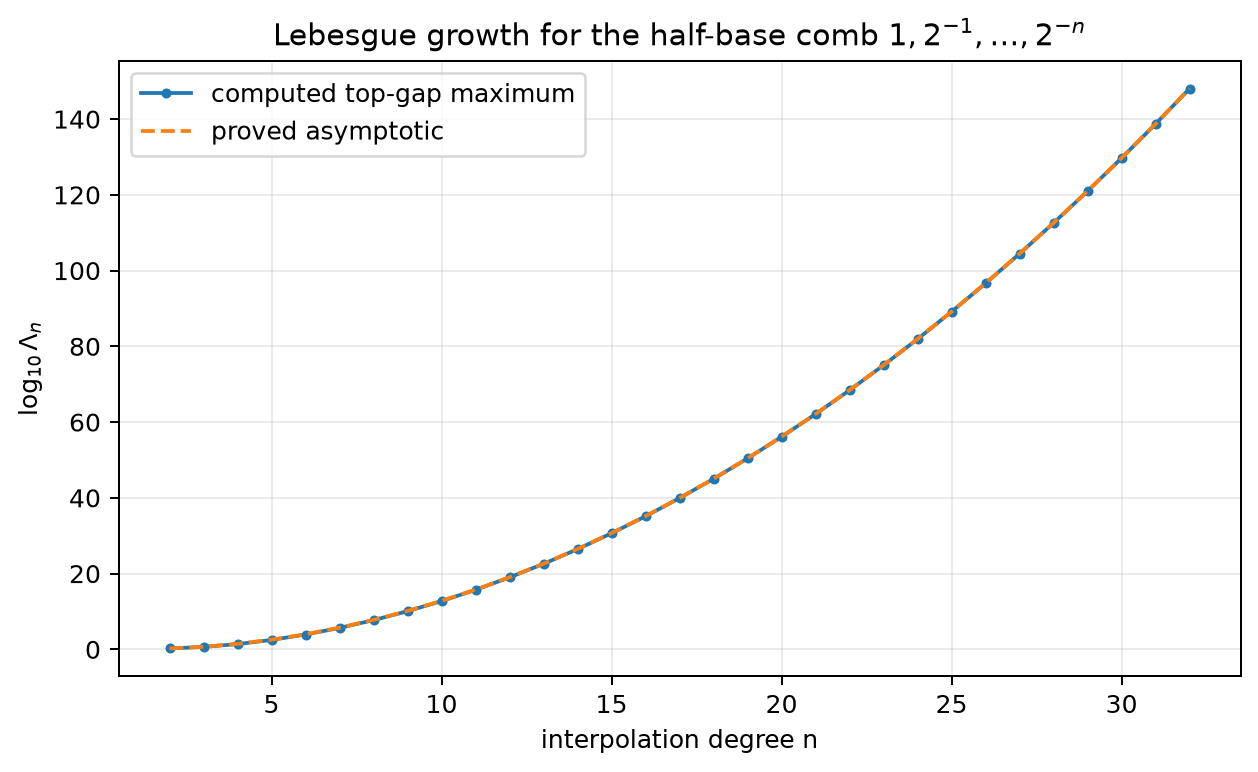
\includegraphics[width=0.90\textwidth]{lebesgue_growth.png}
\caption{Top-gap maxima and the sharp global asymptotic
$2(-q;q)_\infty q^{-\binom n2}/(\EulerE n)$ for $q=1/2$.  Logarithmic arithmetic
is essential: the ordinate already exceeds $10^{148}$ at $n=32$.}
\label{gq:fig:lebesgue-growth}
\end{figure}

\begin{figure}[p]
\centering
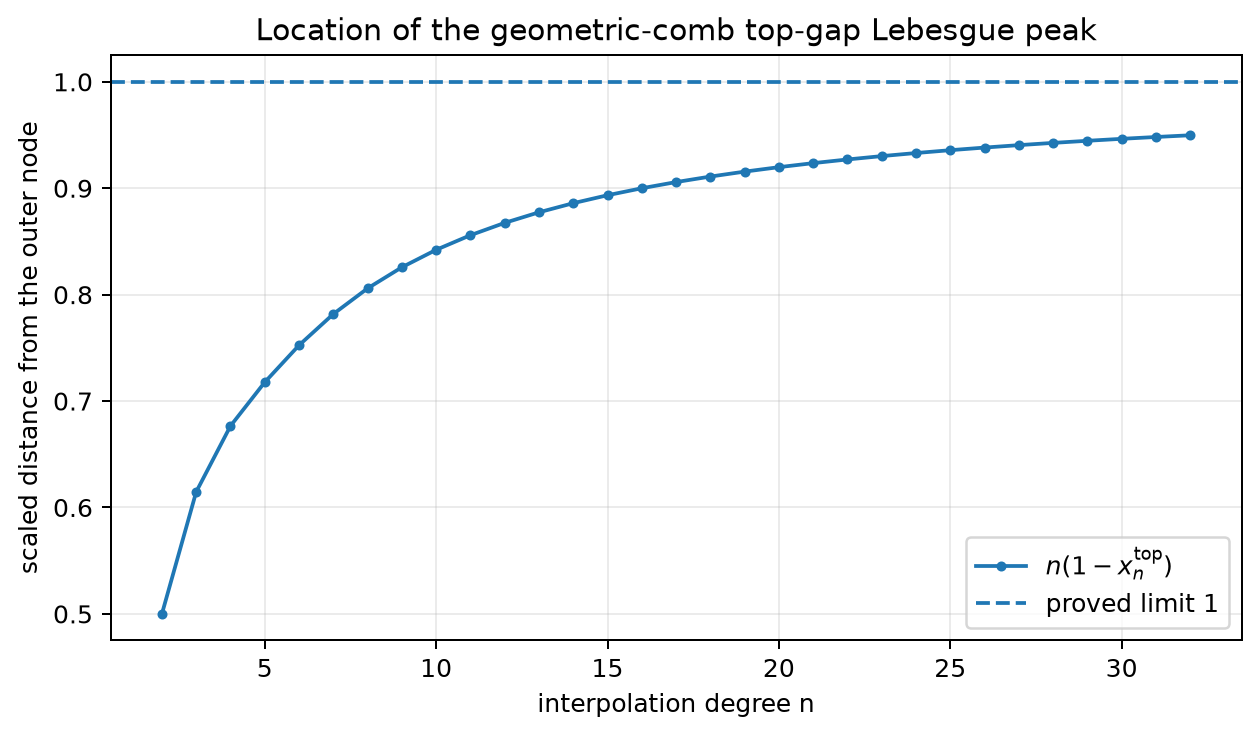
\includegraphics[width=0.90\textwidth]{lebesgue_peak_location.png}
\caption{The scaled top-gap location $n(1-x_n^{\mathrm{top}})$.  The limiting value
$1$ is the maximizer of $\alpha\EulerE^{-\alpha}$ in
\Cref{gq:thm:lebesgue-profile}.}
\label{gq:fig:lebesgue-peak}
\end{figure}

\subsection{Exact Fabius interpolation in the gap}

At $x=3/4$ the target value is exact:
\begin{equation}
 F(3/4)=1-F(1/4)=\frac{67}{72}.
 \label{gq:eq:fabius-three-quarters}
\end{equation}
Every interpolant value in the experiment is a rational number computed
from the exact inverse-dyadic samples.  The error initially fluctuates at a
moderate scale and then enters a clear quadratic-logarithmic growth regime.

\begin{table}[htbp]
\centering
\caption{Exact Fabius interpolation diagnostics.  The third column is the
number of correct decimal digits in the extrapolated boundary value
$R_n=(\Interp_nF)(0)$, measured as $-\log_{10}|R_n|$.}
\label{gq:tab:fabius-numerics}
\small
\begin{tabular}{@{}rrr@{}}
\toprule
$n$ & $\log_{10}|(\Interp_nF)(3/4)-67/72|$ &
$-\log_{10}|R_n|$\\
\midrule
 4 & $-0.8013$ & 2.1595\\
 8 & $ 0.8750$ & 6.7622\\
12 & $ 3.7620$ & 14.3862\\
16 & $10.5655$ & 24.8392\\
20 & $19.0624$ & 37.9904\\
24 & $29.6591$ & 53.8998\\
30 & $49.7229$ & 81.9068\\
40 & $94.5437$ & 140.6070\\
50 & $153.7151$ & 215.2423\\
\bottomrule
\end{tabular}
\end{table}

By $n=50$, the same exact interpolant that predicts $F(0)$ to more than
$215$ decimal digits is wrong at $3/4$ by about $10^{154}$.  This is a
particularly clean numerical manifestation of the stability dichotomy.

\begin{figure}[p]
\centering
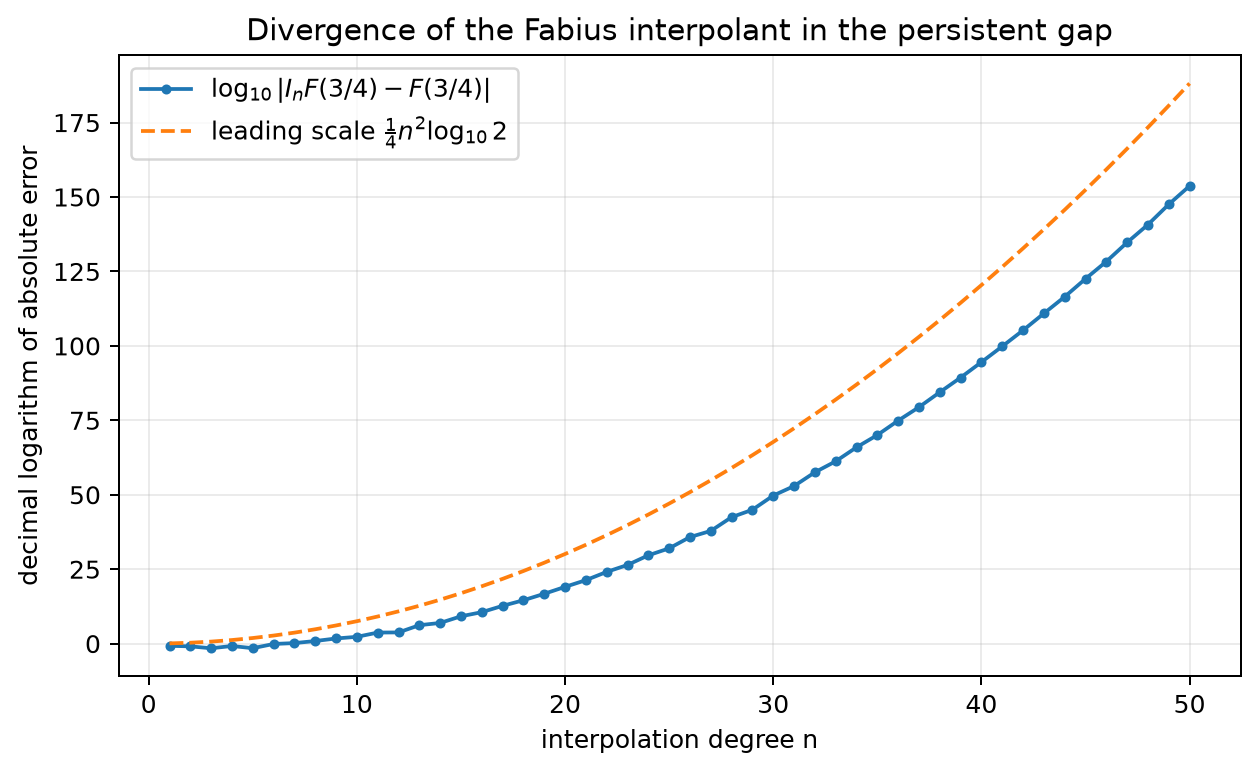
\includegraphics[width=0.90\textwidth]{fabius_gap_divergence.png}
\caption{Exact-rational Fabius interpolation error at $x=3/4$.  The plotted
quadratic comparison is the leading $n^2/4$ term suggested by
\Cref{gq:conj:fabius-gap-asymptotic}; the negative $(n/2)\log n$ correction is
visible as a substantial downward displacement.}
\label{gq:fig:fabius-gap}
\end{figure}

\begin{figure}[p]
\centering
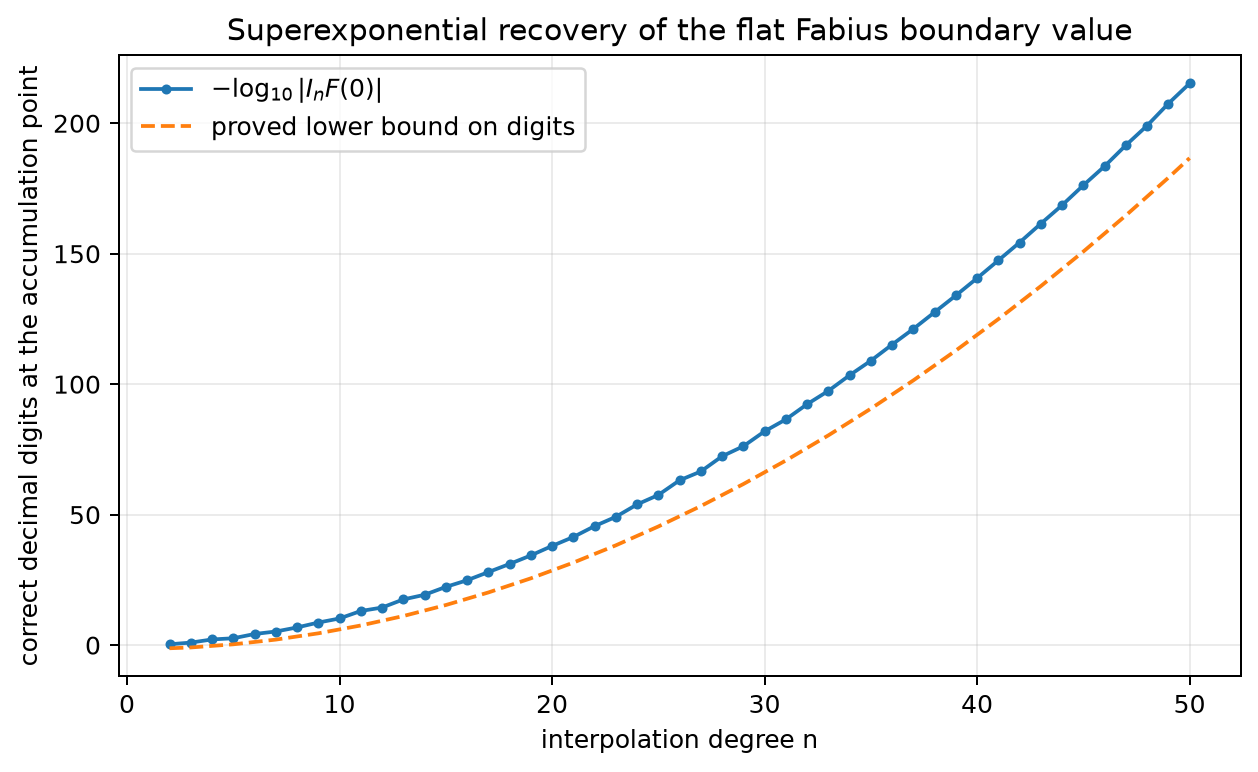
\includegraphics[width=0.90\textwidth]{fabius_boundary_residue.png}
\caption{Decimal digits recovered at the accumulation point.  The exact
residue is compared with the rigorous quadratic-exponential estimate from
\Cref{gq:thm:fabius-boundary-bound}.}
\label{gq:fig:fabius-boundary}
\end{figure}

\begin{observation}[Sign oscillation]
The gap error does not have a simple alternating sign.  Long runs of two
consecutive signs occur, reflecting the motion of a discrete saddle across
integer indices.  This supports the modulation clause in
\Cref{gq:conj:fabius-gap-asymptotic} and argues against fitting a single smooth
prefactor from small $n$.
\end{observation}

\subsection{What the experiments do and do not establish}

The exact checks strongly guard against transcription errors in powers of
$q$, Gaussian reciprocity, and factorial normalizations.  The numerical
top-gap Lebesgue data are consistent with the proved global asymptotic but
are not needed for its proof.
The Fabius gap data, by contrast, are evidence for a conjecture: they show
rapid divergence at one exact rational point but do not prove the proposed
general saddle law.  The script records raw CSV data so alternative
asymptotic fits can be tested without repeating the expensive rational
interpolation.

\section{Further deductions, conjectures, and research directions}
\label{gq:chap:frontiers}

This chapter separates deductions that follow mechanically from the proved
framework from genuinely open asymptotic and structural questions.

\subsection{Second-order Lebesgue asymptotics}

The proof of \Cref{gq:thm:lebesgue-profile} can be expanded one order further.
The factors $(q/x;q)_{n-1}$, the ratio cloud
\eqref{gq:eq:cardinal-ratio}, and $(1-\alpha/n)^{n-1}$ each contribute an
explicit $1/n$ correction.  This suggests the following refinement.

\begin{conjecture}[Second-order boundary layer]
\label{gq:conj:second-order-lebesgue}
There exist explicit constants $A(q)$ and $B(q)$ such that
\begin{align}
 \frac{x_n^*}{c}
 &=1-\frac1n+\frac{A(q)}{n^2}+O_q(n^{-3}),
 \label{gq:eq:second-order-peak-conj}\\
 \Leb_n^*
 &=\frac{2(-q;q)_\infty}{\EulerE}
   \frac{q^{-\binom n2}}{n}
   \left(1+\frac{B(q)}n+O_q(n^{-2})\right).
 \label{gq:eq:second-order-lambda-conj}
\end{align}
The coefficients should be expressible through Lambert series such as
$\sum_{r\ge1}q^r/(1-q^r)$ and weighted Euler-cloud moments.
\end{conjecture}

A proof should follow from a uniform expansion of the ratios of the last
$O(\sqrt{\log n})$ cardinals, with the remainder controlled by the
$q^{\binom r2}$ tail.  The result would turn the qualitative convergence in
\Cref{gq:tab:lebesgue-numerics} into a high-accuracy formula.

\subsection{A function-space criterion for infinite geometric Newton series}

For analytic targets, \Cref{gq:thm:analytic-newton-convergence} supplies a
convenient sufficient condition.  A more intrinsic question starts from a
data sequence $y_j=f(cq^j)$ and asks whether the formal Newton series
\begin{equation}
 \sum_{k\ge0}
 \left(c^{-k}\sum_{j=0}^k
 \frac{(-1)^jq^{-jk+\binom{j+1}{2}}}
 {(q;q)_j(q;q)_{k-j}}y_j\right)N_k(x;c,q)
 \label{gq:eq:formal-data-newton-series}
\end{equation}
converges in a prescribed domain.

\begin{problem}[Geometric Newton sequence spaces]
\label{gq:prob:newton-sequence-spaces}
Characterize weighted sequence spaces $Y$ on the data $y=(y_j)$ and
coefficient spaces $G$ on the divided differences $\gamma=(\gamma_k)$ for
which the triangular Gaussian transform is an isomorphism and the Newton
synthesis map is bounded into $C(K)$, a Hardy space, or a Bergman space.
Determine the exact dependence of the norm on the location of $K$ relative
to the isolated outer node.
\end{problem}

The Richardson generating factorization
\eqref{gq:eq:richardson-generating} indicates that Euler products provide the
correct multipliers on the data side.  A Wiener-algebra formulation may
make inversion and perturbation estimates especially transparent.

\subsection{Signed saddle analysis for Fabius data}

The proof of \Cref{gq:thm:fabius-gap-upper} isolates the unsigned saddle at
\eqref{gq:eq:fabius-saddle-location}.  To prove
\Cref{gq:conj:fabius-gap-asymptotic}, one needs asymptotics for the signed local
packet
\begin{equation}
 \sum_{|j-j_n|\le C\sqrt{\log n}}
 (-1)^j\frac{2^{j(n-j)}a_j}{x-2^{-j}}
 \label{gq:eq:signed-local-saddle-packet}
\end{equation}
with relative error smaller than the packet itself.

A promising route has three stages:
\begin{enumerate}
\item derive uniform saddle asymptotics for $a_j=[z^j]A(z)$ from the product
      \eqref{gq:eq:fabius-mgf-product};
\item insert them into \eqref{gq:eq:signed-local-saddle-packet} and apply a
      discrete Gaussian or theta transformation;
\item retain the fractional saddle displacement, which should produce a
      bounded periodic or antiperiodic modulation.
\end{enumerate}
The functional equation \eqref{gq:eq:fabius-mgf-functional} suggests that the
moment saddle itself carries a logarithmically periodic correction.  Its
interaction with the integer Gaussian saddle may be the source of the sign
blocks seen in the experiment.

\begin{problem}[Exceptional gap points]
\label{gq:prob:exceptional-gap-points}
Determine whether there are points $x\in(1/2,1)$ at which the leading signed
saddle cancels identically or along an infinite subsequence.  If such points
exist, classify them arithmetically and determine the next asymptotic scale.
\end{problem}

\subsection{Boundary-residue entire functions}

The generating function
\begin{equation}
 \mathcal R(z)=(qz;q)_\infty
 \sum_{j\ge0}\frac{q^{\binom j2}a_j}{(q;q)_j}z^j
 \label{gq:eq:boundary-residue-entire-function}
\end{equation}
encodes all endpoint extrapolation errors.  The Euler factor has prescribed
zeros at $z=q^{-r}$, while the second factor is an entire transform of the
Fabius moments.

\begin{problem}[Zero cancellation and coefficient asymptotics]
\label{gq:prob:boundary-entire-zeros}
Determine which Euler zeros survive in $\mathcal R$, obtain the order and
indicator of $\mathcal R$, and use its zero distribution to derive a sharp
asymptotic for $R_n$.  In particular, decide whether
\begin{equation}
 \log|R_n|=-\frac{\log2}{4}n^2+O(n\log n)
 \label{gq:eq:boundary-residue-leading-question}
\end{equation}
has a full expansion with a parity-dependent linear term.
\end{problem}

The exact coefficient formula makes this problem accessible both to
complex-analytic saddle methods and to $2$-adic valuation experiments.

\subsection{Geometric Hermite stability}

The anchored factorization \eqref{gq:eq:anchored-hermite-factorization} removes
confluent linear algebra but not operator growth.  For a flat target, its
data are rescaled by $(cq^j)^{-(m+1)}$, changing the Gaussian saddle.
A first model replaces $a_j$ by
$q^{\binom j2-j(m+1)}a_j$ in the Fabius formulas.  This predicts a movable
saddle and a phase transition when $m$ is allowed to grow with $n$.

\begin{conjecture}[Hermite saddle displacement]
\label{gq:conj:hermite-saddle}
For $q=1/2$ and Fabius data, the dominant index in the gap for the
$m$-anchored interpolant is
\begin{equation}
 j_{n,m}=\frac n2+m+1-\frac{\log n}{2\log2}+O(1),
 \label{gq:eq:hermite-saddle-location-conj}
\end{equation}
until it collides with the endpoint $j=n$.  The collision marks a change
from an interior Gaussian saddle to an endpoint saddle and should determine
the largest useful jet order.
\end{conjecture}

This conjecture follows from the unsigned ratio heuristic; the signed
problem may shift the practical optimum.  It can be tested by extending the
bundled exact code to \Cref{gq:thm:anchored-hermite}.

\subsection{The mixed \texorpdfstring{$q$}{q}-Appell family}

The polynomials $\mathscr A_k(y;c,q)$ in
\eqref{gq:eq:q-Appell-falling} deserve study independently of interpolation.
They combine a Sheffer/Appell deconvolution with a $q$-falling-factorial
basis.

\begin{problem}[Structure of the $q$-Appell falling powers]
\label{gq:prob:q-Appell-structure}
Find:
\begin{enumerate}
\item raising and lowering operators for $\mathscr A_k$ involving $D_q$ and
      the ordinary derivative $D$;
\item their connection coefficients with monomials, ordinary Appell
      polynomials, and $N_k$;
\item generating functions in $k$ and continued-fraction representations;
\item zero-location and interlacing theorems for $0<q<1$;
\item asymptotics in the joint limits $k\to\infty$, $q\to1$, and
      $k(1-q)\to\tau$.
\end{enumerate}
\end{problem}

A useful starting identity is
\begin{equation}
 \sum_{k\ge0}\mathscr A_k(y;c,q)\frac{t^k}{(q;q)_k}
 =\MGF_u(D_y)^{-1}
  \sum_{k\ge0}N_k(y;c,q)\frac{t^k}{(q;q)_k},
 \label{gq:eq:q-Appell-formal-generating}
\end{equation}
where the second series can be rewritten by the infinite $q$-binomial
theorem after normalization.  Making the operator interchange analytic is
itself a worthwhile problem.

\subsection{Decoder variation, total positivity, and optimal gauges}

The matrix $hB$ in \Cref{gq:thm:gaussian-Appell-biorthogonality} is a positive
row-stochastic sampling operator.  Its right inverse $D$ has row sum one but
must use signs.  The size of its row variation controls amplification from
nodal perturbations to atom amplitudes.

\begin{problem}[Minimum-variation atomic decoder]
\label{gq:prob:minimum-variation-decoder}
Among all right inverses of the collocation matrix $hB$, minimize a weighted
$\ell^1$ or total-variation norm subject to exact polynomial reproduction.
Compare the canonical Appell decoder with the minimizer, and determine
whether a symmetry-preserving minimizer has a closed $q$-binomial formula.
\end{problem}

The dense dictionary has an alias kernel inherited from the dyadic Fourier
zeros.  Adding an alias vector changes amplitudes without changing the
synthesized polynomial.  Convex optimization over this affine space may
substantially improve numerical conditioning while preserving every exact
identity.

\subsection{Stable alternatives to global gap interpolation}

The superexponential Lebesgue growth is a property of the all-node global
projector, not of geometric data in general.  Several alternatives retain
the dyadic arithmetic:
\begin{enumerate}
\item piecewise low-degree Newton or Hermite interpolation on geometric
      annuli $[cq^{j+1},cq^j]$;
\item rational barycentric interpolation with fixed local degree;
\item oversampled least squares in a logarithmic coordinate;
\item direct approximation in scaled translates of $\RvachevUp$ rather than first
      passing through one global polynomial;
\item hybrid Taylor--Newton schemes that use the flat germ near zero and a
      separate approximation across the outer gap.
\end{enumerate}
For the Fabius function, the functional equation can transport a local
approximation between adjacent dyadic scales, suggesting multiresolution
algorithms with exact consistency constraints.

\subsection{Complex and arithmetic geometric combs}

When $q$ is complex with $0<|q|<1$, the comb spirals into the origin.  The
algebraic formulas remain valid, while the stability problem becomes
potential-theoretic and angle-dependent.  At a root of unity the nodes
collide and ordinary interpolation becomes confluent; the denominator-free
Gaussian recurrence is then the correct algebraic replacement.

Over finite fields, the condition that $q^0,\ldots,q^n$ be distinct is
exactly an order condition in the multiplicative group.  The geometric
Vandermonde determinant in \Cref{gq:thm:geometric-vandermonde} records its
failure cyclotomically.  This suggests a finite-field interpolation theory
whose transition matrices are literal Gaussian coefficients counting
subspaces.

\begin{problem}[Cyclotomic confluent limit]
\label{gq:prob:cyclotomic-confluent-limit}
Develop a division-free specialization of the cardinal and residual
identities when $q$ approaches a primitive root of unity.  Identify the
resulting Hermite blocks, their cyclotomic valuations, and their relation to
$q$-Lucas congruences.
\end{problem}

\subsection{Formalization program}
\label{gq:sec:formalization-program}

The manuscript layer separates into finite algebra, analytic convergence,
and asymptotics, making the remaining gap well suited to staged
formalization in Lean.  The bullets below distinguish reuse of existing
declarations from genuinely missing statements; they should not be read as
a claim that the whole report is already formalized.

\begin{enumerate}
\item \textbf{Finite products.}  Reuse the existing finite $q$-Pochhammer
      API, then define $N_k$, prove
      \eqref{gq:eq:newton-pochhammer}, and derive the denominator product in
      \Cref{gq:thm:geometric-barycentric} without division until the final
      field specialization.
\item \textbf{Gaussian Pascal equivalence.}  Build on the existing Gaussian
      reciprocity and inversion API to formalize
      \Cref{gq:thm:gaussian-pascal-basis} and its inverse as mutually inverse
      triangular matrices over a commutative ring.
\item \textbf{Residual calculus.}  Reuse the formal complete-homogeneous and
      geometric residual-moment layers to state the arbitrary-evaluation
      interpolation residual; derive the analytic residual only after
      importing convergence lemmas.
\item \textbf{Endpoint stability.}  Reuse the formal rational finite
      $\ell^1$ identity and extend its presentation as needed; the real
      infinite-product limit remains to be formalized.
\item \textbf{Boundary profile.}  Isolate the elementary limits
      $(1-\alpha/n)^n\to\EulerE^{-\alpha}$, dominated convergence for the Euler
      cloud, and the tail bound from $q^{\binom r2}$.
\item \textbf{Fabius arithmetic.}  Reuse the existing exact dyadic-value and
      moment development to prove \Cref{gq:thm:fabius-gaussian-transform}, the
      residue generating function, and the fixed-jet bound.
\item \textbf{Atomic synthesis.}  The generic scalar decoder synthesis,
      coefficient factorization, full interpolation loop, componentwise node
      biorthogonality, and unnormalized decoder row-sum law are formalized in
      \path{FabiusFunction.LagrangeRvachevSynthesis}.  The remaining tasks are
      to derive the geometric elementary-symmetric decoder and Gaussian
      prefactor in
      \eqref{gq:eq:decoder-entry-explicit}--\eqref{gq:eq:decoder-gaussian-prefactor}
      and to package the resulting scalar identities as the Matrix statement
      \eqref{gq:eq:stochastic-right-inverse}.  Decoder optimization remains
      the open problem \Cref{gq:prob:minimum-variation-decoder}.
\end{enumerate}

The sharp global Lebesgue theorem is the most analytically demanding new
formal target.  Its proof was deliberately organized into local profile,
away-from-boundary decay, and compactness of the scaled maximizer so these
pieces can be formalized independently.

\part{Analytic, probabilistic, and Mellin extensions}

\section*{Editorial map of the independent extensions}
\addcontentsline{toc}{section}{Editorial map of the independent extensions}
The finite geometric-comb algebra is stated once in the preceding part. This part retains only the independent material not subsumed by that spine: confluent modal filters, regular variation, geometric-knot splines, geometric-uniform laws, Mellin symbols, superflat divergence, and the reciprocal Rvachev filter.

\section{The Gaussian origin filter as a dilation polynomial}
\label{g1:sec:operator}

The preceding part derives the origin weights from geometric Lagrange
interpolation.  The following compact operator form is the common engine for
the extensions in this part.  For $0<q<1$ put
\begin{align}
 \lambda_{n,k}^{(q)}
 &:={(-1)^{n-k}q^{\binom{n-k+1}{2}}
       \over (q;q)_k(q;q)_{n-k}},
 \qquad 0\le k\le n,
 \label{g1:eq:lambda}\\
 (\Gc_{n,q}f)(A)&:=\sum_{k=0}^n\lambda_{n,k}^{(q)}f(Aq^k).
 \label{g1:eq:G-definition}
\end{align}

\begin{theorem}[Dilation-polynomial factorization]
\label{g1:thm:operator-factorization}
Let $(T_qf)(x)=f(qx)$.  Then
\begin{align}
 W_{n,q}(z):=\sum_{k=0}^n\lambda_{n,k}^{(q)}z^k
 &=\prod_{j=1}^n{z-q^j\over1-q^j},
 \label{g1:eq:row-polynomial}\\
 \Gc_{n,q}=W_{n,q}(T_q)
 &={1\over(q;q)_n}\prod_{j=1}^n(T_q-q^jI),
 \label{g1:eq:operator-factorization}\\
 \Gc_{0,q}=I,
 \qquad
 \Gc_{n,q}&={T_q-q^nI\over1-q^n}\Gc_{n-1,q}.
 \label{g1:eq:operator-recursion}
\end{align}
Consequently the filter can be evaluated in place: starting with
$y_k=f(Aq^k)$, at stage $j=1,\ldots,n$ replace
\begin{equation}
 y_k\longleftarrow{y_{k+1}-q^jy_k\over1-q^j}
 \qquad(0\le k\le n-j).
 \label{g1:eq:triangular-filter}
\end{equation}
The final entry is $(\Gc_{n,q}f)(A)$.
\end{theorem}

\begin{proof}
The finite $q$-binomial theorem expands the product in
\eqref{g1:eq:row-polynomial} and gives exactly the coefficients
\eqref{g1:eq:lambda}.  Substituting the commuting operator $T_q$ for $z$
proves the factorization; separating its last factor proves the recursion.
Applied to the sample vector, that recursion is precisely the in-place update
\eqref{g1:eq:triangular-filter}.
\end{proof}

\begin{corollary}[Exact power multiplier and all integer moments]
\label{g1:cor:power-multiplier}
For $A>0$ and a chosen branch of $A^\alpha,q^\alpha$,
\begin{equation}
 (\Gc_{n,q}x^\alpha)(A)
 =A^\alpha W_{n,q}(q^\alpha)
 =A^\alpha q^{\alpha n}{(q^{1-\alpha};q)_n\over(q;q)_n}.
 \label{g1:eq:pure-power}
\end{equation}
In particular, for every $d\in\NaturalNumbers$,
\begin{equation}
 \sum_{k=0}^n\lambda_{n,k}^{(q)}(Aq^k)^d
 =\begin{cases}
  1,&d=0,\\
  0,&1\le d\le n,\\
  (-1)^nA^dq^{\binom{n+1}{2}}
  \GaussianBinomial{d-1}{n}{q},&d\ge n+1.
 \end{cases}
 \label{g1:eq:all-moments}
\end{equation}
\end{corollary}

\begin{proof}
The function $x^\alpha$ is an eigenfunction of $T_q$ with eigenvalue
$q^\alpha$, so \eqref{g1:eq:row-polynomial} gives the first equality.
Factoring $q^\alpha$ from every numerator factor gives the Pochhammer form.
For integral $d$, its factors give the vanishing range; when $d\ge n+1$,
reversing the factors and using the factorial definition of the Gaussian
coefficient gives \eqref{g1:eq:all-moments}.
\end{proof}

\begin{theorem}[Exact analytic tail and reciprocal-$q$ majorant]
\label{g1:thm:sharp-majorant}
Let $f(z)=\sum_{m\ge0}a_mz^m$.  Formally, and analytically whenever the
series is absolutely convergent,
\begin{equation}
 (\Gc_{n,q}f)(A)-f(0)
 =(-1)^nq^{\binom{n+1}{2}}
  \sum_{r\ge0}\GaussianBinomial{n+r}{n}{q}a_{n+1+r}A^{n+1+r}.
 \label{g1:eq:exact-analytic-tail}
\end{equation}
If $|a_m|\le C R^{-m}$ and $t=|A|/R<1$, then
\begin{equation}
 \left|(\Gc_{n,q}f)(A)-f(0)\right|
 \le Cq^{\binom{n+1}{2}}{t^{n+1}\over(t;q)_{n+1}}.
 \label{g1:eq:sharp-majorant}
\end{equation}
This majorant is coefficientwise sharp: equality in the majorizing sum is
attained when the relevant coefficients have the common phase and magnitudes
$CR^{-m}$.
\end{theorem}

\begin{proof}
Apply \eqref{g1:eq:all-moments} term by term and reindex $m=n+1+r$.
Taking absolute values leaves the series
\[
 Cq^{\binom{n+1}{2}}t^{n+1}
 \sum_{r\ge0}\GaussianBinomial{n+r}{n}{q}t^r.
\]
The reciprocal finite $q$-binomial theorem identifies the last sum with
$(t;q)_{n+1}^{-1}$.  The asserted phase choice makes every triangle
inequality an equality.
\end{proof}

\section{Confluent modal extrapolation}
\label{g1:sec:modal}

Ordinary polynomial cancellation assumes an integer-power Taylor expansion.
Endpoint asymptotics in differential equations, Mellin analysis, and inverse
special functions often contain fractional powers and logarithms.  The
dilation-operator viewpoint gives the correct generalization immediately.

\begin{definition}[Mode polynomial]
Let $\alpha_1,\ldots,\alpha_J\in\ComplexNumbers$ have pairwise distinct spectral
points $q^{\alpha_j}$, none equal to $1$, and let $m_1,\ldots,m_J\in\NaturalNumbers$, and put $N=\sum_jm_j$.  Define
\begin{equation}
 W_{\bm\alpha,\bm m}(z)
 :=\prod_{j=1}^J
 \left(\frac{z-q^{\alpha_j}}{1-q^{\alpha_j}}\right)^{m_j}
 =\sum_{k=0}^Nw_kz^k,
 \label{g1:eq:mode-polynomial}
\end{equation}
and
\[
 (\Rc_{\bm\alpha,\bm m}f)(x):=\sum_{k=0}^Nw_kf(q^kx).
\]
\end{definition}

\begin{theorem}[Confluent annihilation]
The filter \eqref{g1:eq:mode-polynomial} preserves constants and, for every
$j$ and $0\le s<m_j$, annihilates
\[
 x^{\alpha_j}(\log x)^s.
\]
It is the unique filter of degree at most $N$ with these properties.
\end{theorem}

\begin{proof}
For a general polynomial $W(z)=\sum_kw_kz^k$,
\begin{align*}
 \sum_kw_k(q^kx)^\alpha(\log(q^kx))^s
 &=x^\alpha\sum_kw_kq^{k\alpha}
   (\log x+k\log q)^s\\
 &=x^\alpha(\log x+\partial_\alpha)^sW(q^\alpha).
\end{align*}
A zero of multiplicity $m_j$ at $q^{\alpha_j}$ makes the right side vanish for
$s<m_j$.  The normalization $W(1)=1$ preserves constants.  Conversely, the
annihilation equations imply zeros with the stated multiplicities; degree and
normalization then force \eqref{g1:eq:mode-polynomial}.
\end{proof}

\begin{corollary}[Exact general multiplier]
For any $\alpha\in\ComplexNumbers$ and $s\in\NaturalNumbers$,
\begin{equation}
 \Rc_{\bm\alpha,\bm m}
 [x^\alpha(\log x)^s]
 =x^\alpha(\log x+\partial_\alpha)^s
  W_{\bm\alpha,\bm m}(q^\alpha).
 \label{g1:eq:general-mode-multiplier}
\end{equation}
\end{corollary}

\begin{proof}
Because $x^\alpha(\log x)^s=\partial_\alpha^s x^\alpha$ and the
filter is a finite linear combination of dilations, differentiation in
$\alpha$ commutes with the filter.  Apply the pure-power multiplier and
expand $\partial_\alpha^s\!\left(x^\alpha
W_{\bm\alpha,\bm m}(q^\alpha)\right)$ by writing
$\partial_\alpha$ on $x^\alpha$ as multiplication by $\log x$.
\end{proof}

\begin{theorem}[Puiseux--log acceleration]
Suppose, as $x\downarrow0$,
\begin{equation}
 f(x)=a_0+
 \sum_{j=1}^J\sum_{s=0}^{m_j-1}
 a_{j,s}x^{\alpha_j}(\log x)^s
 +O\!\left(x^\beta(1+|\log x|^r)\right),
 \label{g1:eq:puiseux-log-expansion}
\end{equation}
where $\Re\alpha_j>0$ and $\beta>0$.  Then
\begin{equation}
 (\Rc_{\bm\alpha,\bm m}f)(x)
 =a_0+O\!\left(x^\beta(1+|\log x|^r)\right).
 \label{g1:eq:puiseux-acceleration}
\end{equation}
\end{theorem}

\begin{proof}
The finite sum of displayed modes is annihilated exactly.  For each fixed
$k\le N$, replacing $x$ by $q^kx$ preserves the stated remainder order, with a
constant depending on $q,k,\beta,r$.  Summing finitely many weighted remainders
proves the assertion.
\end{proof}

\begin{remark}[Relation to Richardson extrapolation]
This is geometric Richardson extrapolation in its natural spectral form.  The
usual integer-power Gaussian filter corresponds to
$\alpha_j=j$, $m_j=1$.  Repeated exponents handle logarithmic resonance without
introducing derivative data at the nodes.
\end{remark}

\begin{problem}[Stability-optimal modal design]
For a prescribed list of modes, \eqref{g1:eq:mode-polynomial} is algebraically
forced at minimum degree.  If extra degrees of freedom are allowed, determine
the polynomial $W$ with $W(1)=1$ and the required confluent zeros that minimizes
$\sum_k|w_k|$, or a weighted noise norm adapted to the expected precision of
$f(q^kx)$.  This is a finite convex optimization problem whose asymptotic
structure appears unexplored in the Fabius/Rvachev setting.
\end{problem}

\section{Stability, boundary layers, and regular variation}
\label{g1:sec:stability}

\subsection{Exact total variation}

Because the signs of \eqref{g1:eq:lambda} alternate, the total variation can be
read from the row polynomial at $-1$.

\begin{theorem}[Exact noise amplification]
\label{g1:thm:row-norm}
For $0<q<1$,
\begin{equation}
 K_n(q):=\sum_{k=0}^n|\lambda_{n,k}^{(q)}|
 =\frac{(-q;q)_n}{(q;q)_n}
 =\prod_{j=1}^n\frac{1+q^j}{1-q^j}.
 \label{g1:eq:K-n}
\end{equation}
Consequently
\begin{equation}
 K_n(q)\uparrow K_\infty(q):=\frac{(-q;q)_\infty}{(q;q)_\infty}<\infty.
 \label{g1:eq:K-infinity}
\end{equation}
If each sample has absolute error at most $\delta$, the extrapolated absolute
error is at most $K_n(q)\delta$.
\end{theorem}

\begin{proof}
Since
$\Sign\lambda_{n,k}=(-1)^{n-k}$,
\[
 \sum_k|\lambda_{n,k}|=(-1)^n\sum_k\lambda_{n,k}(-1)^k
 =(-1)^nW_{n,q}(-1).
\]
Substitute \eqref{g1:eq:row-polynomial}.  Monotone convergence of the positive
product gives \eqref{g1:eq:K-infinity}.
\end{proof}

For reference,
\[
 K_\infty(1/4)\approx1.9692603537,
 \qquad K_\infty(1/2)\approx8.2559879358,
 \qquad K_\infty(3/4)\approx803.0132718.
\]
Thus the Fourier base $Q=1/4$ associated with dyadic Rvachev scaling is much
better conditioned than a direct dyadic $q=1/2$ extrapolation.

\subsection{The singular regime $q\uparrow1$}

Two limits must be distinguished.  For fixed $n$,
\begin{equation}
 K_n(q)\sim\frac{2^n}{n!(1-q)^n}
 \qquad(q\uparrow1).
 \label{g1:eq:fixed-n-q1}
\end{equation}
If the order tends to infinity first, the growth is nonperturbative.

\begin{theorem}[Modular asymptotic]
Write $q=e^{-t}$ with $t\downarrow0$.  Then
\begin{equation}
 K_\infty(e^{-t})
 \sim\frac{\sqrt t}{2\sqrt\pi}
 \exp\!\left(\frac{\pi^2}{4t}\right).
 \label{g1:eq:K-modular}
\end{equation}
\end{theorem}

\begin{proof}
Use
$(-q;q)_\infty=(q^2;q^2)_\infty/(q;q)_\infty$, so
\[
 K_\infty(q)=\frac{(q^2;q^2)_\infty}{(q;q)_\infty^2}.
\]
The standard Dedekind-eta asymptotic
\[
 (e^{-t};e^{-t})_\infty
 \sim\sqrt{\frac{2\pi}{t}}
 \exp\!\left(-\frac{\pi^2}{6t}+\frac{t}{24}\right)
\]
applied at $t$ and $2t$ gives \eqref{g1:eq:K-modular}; the elementary exponential
corrections cancel.
\end{proof}

The plot in \cref{g1:fig:stability} shows the practical consequence: ratios close
to one are unsuitable for high-order accumulation-point extrapolation unless
precision grows very rapidly.

\subsection{The reversed-row boundary layer}

Put $r=n-k$.  For fixed $r$,
\begin{equation}
 \lambda_{n,n-r}^{(q)}\longrightarrow
 \beta_r^{(q)}:=
 \frac{(-1)^rq^{\binom{r+1}{2}}}{(q;q)_\infty(q;q)_r}.
 \label{g1:eq:beta}
\end{equation}
The limiting signed generating function is
\begin{equation}
 \sum_{r=0}^{\infty}\beta_r^{(q)}z^r
 =\frac{(qz;q)_\infty}{(q;q)_\infty}.
 \label{g1:eq:beta-generating}
\end{equation}
In particular, its mass is $1$ and its total variation is $K_\infty(q)$.

\begin{theorem}[$\ell^1$ boundary-layer convergence]
Extend the reversed row by zero for $r>n$.  Then
\begin{equation}
 \sum_{r=0}^{\infty}
 \left|\lambda_{n,n-r}^{(q)}-\beta_r^{(q)}\right|
 \longrightarrow0.
 \label{g1:eq:l1-boundary}
\end{equation}
\end{theorem}

\begin{proof}
Pointwise convergence follows from $(q;q)_{n-r}\to(q;q)_\infty$.  After
multiplication by $(-1)^r$, all terms are nonnegative.  Their total masses are
$K_n(q)$ and $K_\infty(q)$, respectively, and the former tends to the latter.
Scheffe's lemma for counting measure gives convergence in $\ell^1$.
\end{proof}

This theorem explains the stability mechanism.  For large $n$, the effective
weights sit a bounded number of steps behind the smallest node $Aq^n$; the
large-node coefficients are superexponentially small.

\subsection{Convergence for merely continuous data}

Analyticity is not needed for consistency.

\begin{theorem}[Continuous accumulation-point convergence]
If $f$ is continuous on $[0,A]$, then
\begin{equation}
 (\Gc_{n,q}f)(A)\longrightarrow f(0).
 \label{g1:eq:continuous-convergence}
\end{equation}
More quantitatively, if
$\omega_f(\delta)=\sup_{0\le x\le\delta}|f(x)-f(0)|$, then for
$1\le J\le n+1$,
\begin{align}
 |(\Gc_{n,q}f)(A)-f(0)|
 &\le K_\infty(q)\,\omega_f(Aq^J)\notag\\
 &\quad+\frac{2\|f\|_\infty J}{(q;q)_\infty^2}
 q^{\binom{n-J+2}{2}}.
 \label{g1:eq:modulus-bound}
\end{align}
\end{theorem}

\begin{proof}
Split the weighted sum into $k\ge J$ and $k<J$.  On the first part, every node
is at most $Aq^J$, so the total is bounded by $K_n\omega_f(Aq^J)$.  On the
second part,
\[
 |\lambda_{n,k}^{(q)}|
 \le\frac{q^{\binom{n-k+1}{2}}}{(q;q)_\infty^2}
 \le\frac{q^{\binom{n-J+2}{2}}}{(q;q)_\infty^2}.
\]
There are at most $J$ such terms, and
$|f(Aq^k)-f(0)|\le2\|f\|_\infty$.  First fix $J$ and let $n\to\infty$, then let
$J\to\infty$.
\end{proof}

\subsection{Regularly varying endpoint germs}

A function $f$ is regularly varying at $0+$ with index $\alpha\in\RealNumbers$ if
$f(tx)/f(t)\to x^\alpha$ as $t\downarrow0$ for every $x>0$, with $f$ eventually
of one sign.  Standard background is in \cite{BinghamGoldieTeugels}.

\begin{theorem}[Regular-variation transfer]
Let $f$ be regularly varying at $0+$ with index $\alpha$.  Then, for fixed
$A>0$,
\begin{equation}
 \frac{(\Gc_{n,q}f)(A)}{f(Aq^n)}
 \longrightarrow C_q(\alpha):=
 \frac{(q^{1-\alpha};q)_\infty}{(q;q)_\infty}.
 \label{g1:eq:regular-variation}
\end{equation}
For a positive integer $\alpha=m$, the limit is zero because the numerator
product contains the factor $1-q^0$.
\end{theorem}

\begin{proof}
Reverse the row:
\[
 \frac{(\Gc_{n,q}f)(A)}{f(Aq^n)}
 =\sum_{r=0}^n\lambda_{n,n-r}^{(q)}
   \frac{f(Aq^{n-r})}{f(Aq^n)}.
\]
For fixed $r$, regular variation gives a limit $q^{-\alpha r}$, while
\eqref{g1:eq:beta} gives the coefficient limit.  Potter bounds dominate the
ratio by $Cq^{-(\alpha+\varepsilon)r}$ away from a finite initial segment; the
factor $q^{r(r+1)/2}$ in $\beta_r$ makes the resulting series summable for every
$\alpha$.  The finitely many terms corresponding to nodes bounded away from
zero have superexponentially small coefficients.  Dominated convergence and
\eqref{g1:eq:beta-generating} now give
\[
 \sum_{r\ge0}\beta_r^{(q)}q^{-\alpha r}
 =\frac{(q^{1-\alpha};q)_\infty}{(q;q)_\infty}.
\]
\end{proof}

For pure powers, \eqref{g1:eq:regular-variation} is already visible in the exact
formula \eqref{g1:eq:pure-power}.  The theorem says that slowly varying factors do
not change the limiting multiplier.

\section{Smooth remainders and geometric-knot B-splines}
\label{g1:sec:bspline}

\subsection{Hermite--Genocchi representation}

The exact Taylor tail is best for analytic data.  For finite smoothness, a
divided-difference representation reveals positivity and sign.

\begin{theorem}[Geometric Hermite--Genocchi remainder]
Let $f\in C^{n+1}[0,A]$ and let
$(T_*,T_0,\ldots,T_n)$ be uniformly distributed on the $(n+1)$-simplex,
that is, Dirichlet with all parameters equal to $1$.  Put
\begin{equation}
 Y_{n,A,q}:=A\sum_{k=0}^nq^kT_k.
 \label{g1:eq:Y-dirichlet}
\end{equation}
Then
\begin{equation}
 (\Gc_{n,q}f)(A)-f(0)
 =\frac{(-1)^nA^{n+1}q^{\binom{n+1}{2}}}{(n+1)!}
 \Expectation\bigl[f^{(n+1)}(Y_{n,A,q})\bigr].
 \label{g1:eq:HG-remainder}
\end{equation}
\end{theorem}

\begin{proof}
Let $I_nf$ be the interpolating polynomial through $A,Aq,\ldots,Aq^n$.
The ordinary interpolation remainder at $0$ gives
\begin{align*}
 I_nf(0)-f(0)
 &=(-1)^nA^{n+1}q^{\binom{n+1}{2}}
 f[0,A,Aq,\ldots,Aq^n].
\end{align*}
The Hermite--Genocchi formula for a divided difference of order $n+1$ is
\[
 f[0,A,Aq,\ldots,Aq^n]
 =\frac1{(n+1)!}
 \Expectation f^{(n+1)}\!\left(A\sum_{k=0}^nq^kT_k\right).
\]
Since $I_nf(0)=(\Gc_{n,q}f)(A)$, the result follows.
\end{proof}

\begin{corollary}[Sharp derivative bound and sign]
Under the hypotheses of the theorem,
\begin{equation}
 |(\Gc_{n,q}f)(A)-f(0)|
 \le\frac{A^{n+1}q^{\binom{n+1}{2}}}{(n+1)!}
 \|f^{(n+1)}\|_{L^\infty(0,A)}.
 \label{g1:eq:smooth-bound}
\end{equation}
If $f^{(n+1)}$ has a fixed nonzero sign on $(0,A)$, then the remainder has the
sign of $(-1)^nf^{(n+1)}$.
\end{corollary}

\begin{proof}
The Hermite--Genocchi formula expresses the remainder as
$(-1)^nA^{n+1}q^{\binom{n+1}{2}}/(n+1)!$ times an average of
$f^{(n+1)}$ over points in $[0,A]$.  Taking absolute values gives the
bound, while a fixed nonzero sign of the derivative fixes the sign of
that average.
\end{proof}

\subsection{Peano kernel and a positive spline density}

For $n\ge1$, define the Peano kernel
\begin{equation}
 K_{n,A,q}(t):=\frac1{n!}\sum_{k=0}^n
 \lambda_{n,k}^{(q)}(Aq^k-t)_+^n,
 \qquad 0\le t\le A.
 \label{g1:eq:Peano-kernel}
\end{equation}
Then
\[
 (\Gc_{n,q}f)(A)-f(0)=\int_0^Af^{(n+1)}(t)K_{n,A,q}(t)\Differential t.
\]
Normalize it by
\begin{equation}
 B_{n,A,q}(t):=
 \frac{(-1)^n(n+1)!}{A^{n+1}q^{\binom{n+1}{2}}}K_{n,A,q}(t).
 \label{g1:eq:B-density}
\end{equation}

\begin{theorem}[Geometric-knot B-spline]
The function $B_{n,A,q}$ is the probability density of
$Y_{n,A,q}$ in \eqref{g1:eq:Y-dirichlet}.  In particular,
\begin{enumerate}[label=(\roman*),leftmargin=2em]
\item $B_{n,A,q}\ge0$ and is supported on $[0,A]$;
\item $\int_0^AB_{n,A,q}(t)\Differential t=1$;
\item it is the classical univariate B-spline associated with the knots
$0,Aq^n,\ldots,Aq,A$, up to the displayed normalization;
\item it is log-concave and hence unimodal on the interior of its support.
\end{enumerate}
\end{theorem}

\begin{proof}
Comparing the Peano representation with \eqref{g1:eq:HG-remainder} for arbitrary
continuous $f^{(n+1)}$ identifies the normalized kernel with the law of
$Y_{n,A,q}$.  This is also the standard Curry--Schoenberg interpretation of a
B-spline as the density of a Dirichlet average of its knots; see
\cite{deBoor}.  Positivity, support, and normalization follow immediately.
The uniform density on a simplex is log-concave, and linear images preserve
log-concavity by the Prekopa theorem, proving the last assertion.
\end{proof}

\begin{remark}[Not the same as a ``quantum B-spline'']
The density above is a classical B-spline whose knots happen to be geometric.
It should be distinguished from the quantum B-splines of
Simeonov--Goldman \cite{SimeonovGoldman}, where continuity conditions are
formulated using $q$-derivatives.  The two theories meet through divided
differences and Jackson calculus, but their definitions are different.  The
geometric-knot density is the one canonically forced by the interpolation
remainder in this report.
\end{remark}

\subsection{Exact moments}

\begin{theorem}[Gaussian-binomial B-spline moments]
For every $r\in\NaturalNumbers$,
\begin{equation}
 \Expectation Y_{n,A,q}^r
 =\frac{r!(n+1)!}{(n+r+1)!}
 A^r\GaussianBinomial{n+r}{n}{q}.
 \label{g1:eq:Y-moments}
\end{equation}
Equivalently,
\begin{equation}
 \int_0^At^rB_{n,A,q}(t)\Differential t
 =\frac{r!(n+1)!}{(n+r+1)!}
 A^r\GaussianBinomial{n+r}{n}{q}.
\end{equation}
\end{theorem}

\begin{proof}
For a Dirichlet$(1,\ldots,1)$ vector with $n+2$ components,
\[
 \Expectation\left(\sum_i x_iT_i\right)^r
 =\frac{r!(n+1)!}{(n+r+1)!}h_r(x_0,\ldots,x_{n+1}).
\]
Take the knots $0,A,Aq,\ldots,Aq^n$ and apply
\eqref{gq:eq:h-principal}.
\end{proof}

Thus the Gaussian coefficient is not only an interpolation residual: it is the
moment sequence of the positive Peano-kernel distribution after a simple beta
normalization.

\subsection{A $q$-Pochhammer scaling limit}

The geometric B-spline has a nontrivial boundary-scale limit.  Let
$E_*,E_0,E_1,\ldots$ be independent exponential random variables of mean $1$.

\begin{theorem}[Scaling limit of the geometric B-spline]
For fixed $0<q<1$,
\begin{equation}
 \frac{n+2}{A}Y_{n,A,q}
 \xrightarrow{\ d\ }
 Z_q:=\sum_{k=0}^{\infty}q^kE_k.
 \label{g1:eq:Y-scaling-limit}
\end{equation}
The limit has moments and Laplace transform
\begin{align}
 \Expectation Z_q^r&=\frac{r!}{(q;q)_r},
 \label{g1:eq:Z-moments}\\
 \Expectation e^{-sZ_q}&=\frac1{(-s;q)_\infty},\qquad s\ge0.
 \label{g1:eq:Z-Laplace}
\end{align}
For $y>0$ its density admits the absolutely convergent expansion
\begin{equation}
 p_q(y)=\frac1{(q;q)_\infty}
 \sum_{k=0}^{\infty}
 \frac{(-1)^kq^{\binom{k}{2}}}{(q;q)_k}
 e^{-q^{-k}y}.
 \label{g1:eq:Z-density}
\end{equation}
\end{theorem}

\begin{proof}
Use the exponential representation of a uniform Dirichlet vector:
\[
 (T_*,T_0,\ldots,T_n)
 \overset d=
 \frac{(E_*,E_0,\ldots,E_n)}{E_*+E_0+\cdots+E_n}.
\]
The denominator divided by $n+2$ converges almost surely to $1$, while
$\sum_{k=0}^nq^kE_k$ converges almost surely and in every $L^r$ to $Z_q$.
Slutsky's theorem proves \eqref{g1:eq:Y-scaling-limit}.  Independence gives
\[
 \Expectation e^{-sZ_q}=\prod_{k\ge0}(1+sq^k)^{-1}=(-s;q)_\infty^{-1}.
\]
Expanding $1/(t;q)_\infty=\sum_{r\ge0}t^r/(q;q)_r$ around $t=0$ and comparing
moment-generating coefficients gives \eqref{g1:eq:Z-moments}.

For the density, first decompose the finite product
$\prod_{j=0}^{N}(1+sq^j)^{-1}$ into simple fractions.  Its coefficient at the
pole $s=-q^{-k}$ is the finite version of
\[
 \frac1{(-s;q)_\infty}
 =\sum_{k\ge0}
 \frac{(-1)^kq^{\binom{k+1}{2}}}
 {(q;q)_k(q;q)_\infty}\frac1{1+sq^k}.
\]
For $s\ge0$, the finite coefficients converge to the displayed coefficients
and are dominated by a constant times
$q^{\binom{k+1}{2}}/(q;q)_k$; dominated convergence therefore gives the
infinite partial-fraction identity.  Termwise Laplace inversion gives
\eqref{g1:eq:Z-density}.  For each $y>0$, the Gaussian factor in $k$ together with
$e^{-q^{-k}y}$ gives absolute convergence and justifies the inversion.
\end{proof}

\begin{remark}
The limit satisfies the perpetuity equation
\[
 Z_q\overset d=E_0+qZ_q',
\]
where $Z_q'$ is an independent copy.  The $q$-Pochhammer product is therefore
both an interpolation object and the Laplace transform of the boundary-scale
limit of the associated B-splines.
\end{remark}

\section{Geometric-uniform random sums and finite splines}
\label{g1:sec:uniform-sums}

\subsection{The generic law}

Let $0<b<1$ and let $U_0,U_1,\ldots$ be independent uniforms on $[0,1]$.
Define
\begin{equation}
 X_b:=(1-b)\sum_{j=0}^{\infty}b^jU_j.
 \label{g1:eq:Xb}
\end{equation}
The weights sum to $1$, so $X_b\in[0,1]$.  Splitting off the first summand gives
the distributional self-similarity
\begin{equation}
 X_b\overset d=(1-b)U_0+bX_b',
 \label{g1:eq:Xb-selfsimilar}
\end{equation}
where $X_b'$ is an independent copy.  If $F_b$ is the distribution function,
then
\begin{equation}
 F_b(x)=\int_0^1F_b\!\left(\frac{x-(1-b)u}{b}\right)\Differential u,
 \label{g1:eq:Fb-integral}
\end{equation}
with the conventions $F_b=0$ to the left of $0$ and $F_b=1$ to the right of
$1$.  At $b=1/2$, this is the Fabius distribution.

\subsection{Finite generalized Irwin--Hall splines}

Let
\[
 X_{b,N}:=(1-b)\sum_{j=0}^{N-1}b^jU_j,
 \qquad a_j=(1-b)b^j.
\]
This is a convolution of uniforms on intervals of geometrically decreasing
width.

\begin{theorem}[Finite box-spline formula]
For $N\ge1$, the density and distribution function of $X_{b,N}$ are
\begin{align}
 f_{b,N}(x)
 &=\frac1{(N-1)!\prod_{j=0}^{N-1}a_j}
 \sum_{\varepsilon\in\{0,1\}^N}
 (-1)^{|\varepsilon|}
 \left(x-\sum_{j=0}^{N-1}\varepsilon_ja_j\right)_+^{N-1},
 \label{g1:eq:finite-density}\\
 F_{b,N}(x)
 &=\frac1{N!\prod_{j=0}^{N-1}a_j}
 \sum_{\varepsilon\in\{0,1\}^N}
 (-1)^{|\varepsilon|}
 \left(x-\sum_{j=0}^{N-1}\varepsilon_ja_j\right)_+^N,
 \label{g1:eq:finite-CDF}
\end{align}
where
\begin{equation}
 \prod_{j=0}^{N-1}a_j=(1-b)^Nb^{N(N-1)/2}.
 \label{g1:eq:product-widths}
\end{equation}
\end{theorem}

\begin{proof}
The density of a uniform on $[0,a]$ is
$a^{-1}(H(x)-H(x-a))$, where $H$ is the Heaviside function.  Convolving $N$
such factors and expanding the product of translation differences gives the
alternating subset sum.  The $N$-fold convolution of $H$ is
$x_+^{N-1}/(N-1)!$.  Integration gives the CDF, and
\eqref{g1:eq:product-widths} is immediate.
\end{proof}

For a general $b$, the knots are subset sums of a geometric progression.  At
the dyadic value they collapse to an arithmetic comb, and the coefficient sign
is the Thue--Morse sign.

\begin{corollary}[Dyadic Thue--Morse collapse]
For $b=1/2$,
\begin{equation}
 F_{1/2,N}(x)
 =\frac{2^{N(N+1)/2}}{N!}
 \sum_{r=0}^{2^N-1}(-1)^{\BinaryDigitSum(r)}
 \left(x-\frac{r}{2^N}\right)_+^N,
 \label{g1:eq:dyadic-finite-CDF}
\end{equation}
where $\BinaryDigitSum(r)$ is the binary digit sum of $r$.
\end{corollary}

\begin{proof}
Here $a_j=2^{-(j+1)}$.  Every subset sum is uniquely $r/2^N$, and the subset
cardinality has the parity of $\BinaryDigitSum(r)$.  The product of widths is
$2^{-N(N+1)/2}$.
\end{proof}

This identity explains why a geometric collection of widths produces an
arithmetic dyadic knot comb: binary representation converts subset selection
into position on the uniform grid, while the inclusion--exclusion sign becomes
the Thue--Morse sequence.

\subsection{Convergence to the infinite law}

The omitted tail is bounded deterministically:
\[
 0\le X_b-X_{b,N}\le b^N.
\]
Hence
\begin{equation}
 F_b(x)\le F_{b,N}(x)\le F_b(x+b^N).
 \label{g1:eq:CDF-sandwich}
\end{equation}
Because $F_b$ is continuous, $F_{b,N}\to F_b$ uniformly.  Thus the Fabius
function is a uniform limit of explicitly known compactly supported splines
whose coefficients are a Thue--Morse finite difference.

\subsection{Centered law, Bernoulli cumulants, and sinc products}

Put
\begin{equation}
 Z_b:=2X_b-1
 =2(1-b)\sum_{j=0}^{\infty}b^j(U_j-1/2).
 \label{g1:eq:Zb}
\end{equation}
Then $Z_b$ is symmetric and supported on $[-1,1]$.  Under the Fourier
convention
\[
 \FourierTwoPi{u_b}(z)=\Expectation\,\EulerE^{-2\pi\ImaginaryUnit zZ_b},
\]
its characteristic function is
\begin{equation}
 \FourierTwoPi{u_b}(z)
 =\prod_{j=0}^{\infty}
 \SincRad\!\bigl(2\pi(1-b)b^jz\bigr),
 \qquad \SincRad w:=\frac{\sin w}{w}.
 \label{g1:eq:generic-sinc-product}
\end{equation}
At $b=1/2$, this is
\begin{equation}
 \FourierTwoPi{\RvachevUp}(z)=\prod_{j=0}^{\infty}\SincRad(\pi z/2^j),
 \label{g1:eq:up-sinc}
\end{equation}
which is the standard Rvachev product.

The centered uniform on $[-1/2,1/2]$ has cumulants
$\kappa_m=B_m/m$ for $m\ge2$, where $B_m$ are Bernoulli numbers and odd
cumulants vanish.  Independence and scaling give the following explicit
$q$-denominators.

\begin{proposition}[Cumulants of the geometric-uniform law]
For $m\ge1$,
\begin{equation}
 \kappa_{2m}(Z_b)
 =\frac{[2(1-b)]^{2m}B_{2m}}
 {2m(1-b^{2m})},
 \qquad \kappa_{2m+1}(Z_b)=0.
 \label{g1:eq:Zb-cumulants}
\end{equation}
Consequently every even moment is an explicit complete Bell polynomial in the
numbers \eqref{g1:eq:Zb-cumulants}.
\end{proposition}

\begin{proof}
Cumulants add under independent sums and scale homogeneously.  Therefore
\[
 \kappa_{2m}(Z_b)
 =[2(1-b)]^{2m}\frac{B_{2m}}{2m}
 \sum_{j\ge0}b^{2mj},
\]
and the geometric sum gives \eqref{g1:eq:Zb-cumulants}.
\end{proof}

The factors $1-b^{2m}$ are the simplest $q$-analog denominators.  In Fourier
space the same even degree $2m$ is responsible for the squared interpolation
base developed in \cref{g1:sec:fourier}.

\section{Fabius and Rvachev functions at the flat boundary}
\label{g1:sec:fabius}

\subsection{Definitions and endpoint differential scaling}

Let $F$ be the Fabius distribution function on $[0,1]$.  It is the CDF of
$X_{1/2}$ and satisfies
\begin{equation}
 F(0)=0,\qquad F(1)=1,\qquad F(1-x)=1-F(x),
 \label{g1:eq:F-symmetry}
\end{equation}
and, for $0\le x\le1/2$,
\begin{equation}
 F'(x)=2F(2x).
 \label{g1:eq:F-DE}
\end{equation}
The compactly supported Rvachev function is related by
\begin{equation}
 \RvachevUp(x)=F(1-|x|),\qquad |x|\le1,
 \label{g1:eq:Up-F}
\end{equation}
with $\RvachevUp(x)=0$ for $|x|\ge1$.  These normalizations agree with the primary
Fabius/Rvachev literature \cite{Fabius1966,Rvachev1990,AriasDeReyna} and with
the inspected ProveIt exposition \cite{ProveItFabius}.

Repeated differentiation of \eqref{g1:eq:F-DE} gives the exact endpoint scaling.

\begin{lemma}[Endpoint derivatives]
For $m\ge1$ and $0\le x\le2^{-m}$,
\begin{equation}
 F^{(m)}(x)=2^{m(m+1)/2}F(2^mx).
 \label{g1:eq:F-derivatives}
\end{equation}
\end{lemma}

\begin{proof}
The case $m=1$ is \eqref{g1:eq:F-DE}.  If the result holds for $m$, then on
$x\le2^{-(m+1)}$,
\[
 F^{(m+1)}(x)=2^{m(m+1)/2}2^mF'(2^mx)
 =2^{m(m+1)/2+m+1}F(2^{m+1}x),
\]
which has exponent $(m+1)(m+2)/2$.
\end{proof}

\subsection{An exact boundary-comb identity}

The smooth Peano remainder becomes self-similar when $f=F$.

\begin{theorem}[Fabius boundary filter]
Let $n\ge0$, $0<A\le2^{-(n+1)}$, and let
$(T_*,T_0,\ldots,T_n)$ be uniform Dirichlet.  Put
\begin{equation}
 S_n:=\sum_{k=0}^n2^{-k}T_k\in[0,1].
 \label{g1:eq:Sn}
\end{equation}
Then
\begin{equation}
 \sum_{k=0}^n\lambda_{n,k}^{(1/2)}F(A2^{-k})
 =\frac{(-1)^n(2A)^{n+1}}{(n+1)!}
 \Expectation F(2^{n+1}AS_n).
 \label{g1:eq:F-boundary-filter}
\end{equation}
In particular, the left side has strict sign $(-1)^n$ and obeys
\begin{equation}
 0<(-1)^n\sum_{k=0}^n\lambda_{n,k}^{(1/2)}F(A2^{-k})
 \le\frac{(2A)^{n+1}}{(n+1)!}.
 \label{g1:eq:F-boundary-bound}
\end{equation}
\end{theorem}

\begin{proof}
Apply \eqref{g1:eq:HG-remainder} with $q=1/2$ and $f=F$.  Since $F(0)=0$,
\[
 \sum_k\lambda_{n,k}^{(1/2)}F(A2^{-k})
 =\frac{(-1)^nA^{n+1}2^{-n(n+1)/2}}{(n+1)!}
 \Expectation F^{(n+1)}(AS_n).
\]
The hypothesis on $A$ allows \eqref{g1:eq:F-derivatives} with $m=n+1$ throughout
the support of $AS_n$.  The powers of $2$ reduce to $2^{n+1}$, giving
\eqref{g1:eq:F-boundary-filter}.  The random argument lies in $[0,1]$, so
$0\le F\le1$.  It is positive almost surely because $S_n>0$ almost surely,
which gives strict sign and the bound.
\end{proof}

\begin{corollary}[Exact dyadic form]
If $M\ge n+1$, then
\begin{equation}
 \sum_{k=0}^n\lambda_{n,k}^{(1/2)}F(2^{-(M+k)})
 =\frac{(-1)^n2^{-(M-1)(n+1)}}{(n+1)!}
 \Expectation F(2^{n+1-M}S_n).
 \label{g1:eq:F-dyadic-filter}
\end{equation}
For $M=n+1$, the ratio of the absolute value to the upper bound is exactly
$\Expectation F(S_n)$.
\end{corollary}

\begin{proof}
Set $A=2^{-M}$ in \cref{g1:eq:F-boundary-filter}; the hypothesis
$M\ge n+1$ is exactly the required boundary-range condition.  Then
$(2A)^{n+1}=2^{-(M-1)(n+1)}$, proving the formula.  At $M=n+1$ the
argument of $F$ is $S_n$, and division by the preceding theorem's upper
bound leaves precisely $\Expectation F(S_n)$.
\end{proof}

Through \eqref{g1:eq:Up-F}, the same result is an identity on the left boundary of
$\RvachevUp$:
\begin{equation}
 \sum_{k=0}^n\lambda_{n,k}^{(1/2)}
 \RvachevUp(-1+A2^{-k})
 =\frac{(-1)^n(2A)^{n+1}}{(n+1)!}
 \Expectation F(2^{n+1}AS_n).
 \label{g1:eq:Up-boundary-filter}
\end{equation}
Thus a signed combination of values of a nowhere-analytic $C^\infty$ function
is represented by a positive expectation and has a completely determined
sign.

\subsection{The boundary B-spline and its $q$-exponential scale}

The variable $S_n$ is $Y_{n,1,1/2}$ from \cref{g1:sec:bspline}.  Therefore
\begin{equation}
 (n+2)S_n\xrightarrow{d}Z_{1/2}
 =\sum_{k\ge0}2^{-k}E_k,
 \qquad
 \Expectation e^{-sZ_{1/2}}=\frac1{(-s;1/2)_\infty}.
 \label{g1:eq:Sn-limit}
\end{equation}
This identifies the random scale sampled by the normalized Fabius remainder.
The typical size of $S_n$ is $2/(n+2)$, but its limiting rescaled distribution
is not degenerate; it is the $q$-Pochhammer perpetuity in
\eqref{g1:eq:Z-Laplace}.

\subsection{Exact rational computation}

All dyadic values of $F$ are rational.  A convenient triangular recurrence,
also used in the linked monograph, is
\begin{equation}
 V_0=1,\qquad
 V_m:=F(2^{-m})
 =\frac{2^{-\binom m2}}{2^m-1}
 \sum_{k=0}^{m-1}
 \frac{2^{\binom k2}}{(m-k+1)!}V_k.
 \label{g1:eq:V-recurrence}
\end{equation}
It begins
\[
 V_0=1,\quad V_1=\frac12,\quad V_2=\frac5{72},\quad
 V_3=\frac1{288},\quad V_4=\frac{143}{2073600}.
\]
Because both \eqref{g1:eq:V-recurrence} and the dyadic weights
$\lambda_{n,k}^{(1/2)}$ are rational, \eqref{g1:eq:F-dyadic-filter} can be checked
with exact integer arithmetic.  The companion Python program does so before
switching to multiprecision arithmetic for larger plotted orders.

\section{Fourier-scale interpolation for the Rvachev function}
\label{g1:sec:fourier}

\subsection{The base-squaring principle}

Let $\Phi$ be an even entire function normalized by $\Phi(0)=1$, and write
\begin{equation}
 \Phi(z)=\sum_{m=0}^{\infty}c_mz^{2m}.
 \label{g1:eq:Phi-even}
\end{equation}
Fix a scale ratio $0<c<1$ and set
\begin{equation}
 Q:=c^2,\qquad H_z(t):=\Phi(z\sqrt t)
 =\sum_{m=0}^{\infty}c_mz^{2m}t^m.
 \label{g1:eq:Hzt}
\end{equation}
Evenness makes $H_z$ entire in $t$, independent of the choice of square root.
Moreover
\begin{equation}
 H_z(Q^k)=\Phi(c^kz).
 \label{g1:eq:scale-samples}
\end{equation}
Therefore geometric interpolation of Fourier scales $c^kz$ is interpolation on
the comb $1,Q,Q^2,\ldots$, not on base $c$ itself.  In the dyadic Rvachev
problem, $c=1/2$ and the interpolation base is $Q=1/4$.

\subsection{Exact moment-flat filter}

Let $\lambda_{n,k}^{(Q)}$ denote the origin weights with base $Q$.

\begin{theorem}[Even-entire scale filter]
For $H_z$ as in \eqref{g1:eq:Hzt},
\begin{align}
 \sum_{k=0}^n\lambda_{n,k}^{(Q)}\Phi(c^kz)
 &=1+(-1)^nQ^{\binom{n+1}{2}}
 \sum_{r=0}^{\infty}\GaussianBinomial{n+r}{n}{Q}
 c_{n+1+r}z^{2n+2+2r}.
 \label{g1:eq:even-entire-filter}
\end{align}
In particular, the residual has a zero of order at least $2n+2$ at $z=0$.
\end{theorem}

\begin{proof}
Apply \eqref{g1:eq:exact-analytic-tail} to the entire function $H_z(t)$ at
$A=1$ and base $Q$.
\end{proof}

For a characteristic function under the convention
$\Phi(z)=\Expectation e^{-2\pi izX}$ with a symmetric random variable $X$,
\begin{equation}
 c_m=(-1)^m\frac{(2\pi)^{2m}\mu_{2m}}{(2m)!},
 \qquad \mu_{2m}=\Expectation X^{2m}.
 \label{g1:eq:Fourier-coeff-moments}
\end{equation}
Hence the first nonzero term of the filtered residual is always
\begin{equation}
 -Q^{\binom{n+1}{2}}
 \frac{(2\pi z)^{2n+2}\mu_{2n+2}}{(2n+2)!}.
 \label{g1:eq:leading-Fourier-residual}
\end{equation}
For real $z$ near zero this is negative, regardless of the parity of $n$.

\subsection{Application to $\RvachevUp$}

For the Rvachev function,
\[
 \Phi(z)=\FourierTwoPi{\RvachevUp}(z)
 =\prod_{j=0}^{\infty}\SincRad(\pi z/2^j).
\]
Taking $c=1/2$ and $Q=1/4$ in
\eqref{g1:eq:even-entire-filter} gives an exact finite multiscale identity.  Its
uniform sample-noise amplification is bounded by
$K_\infty(1/4)\approx1.96926$, which is notably mild.

More generally, the centered geometric-uniform density $u_b$ in
\eqref{g1:eq:generic-sinc-product} has an even transform, and samples at scales
$b^kz$ are governed by the interpolation base $Q=b^2$.  The cumulants
\eqref{g1:eq:Zb-cumulants} determine the coefficients through Bell polynomials,
so the filter simultaneously links Gaussian coefficients, Bernoulli numbers,
Bell polynomials, and the infinite sinc product.

\subsection{Entire Newton reconstruction of all scales}

The finite filter recovers the constant term approximately.  The infinite
Newton series reconstructs the complete scale function.

\begin{theorem}[Scale reconstruction from a geometric sample ray]
Let $\Phi$ be even entire, fix $z\in\ComplexNumbers$, and set $H_z$ by
\eqref{g1:eq:Hzt}.  Then for every $t\in\ComplexNumbers$,
\begin{equation}
 \Phi(z\sqrt t)
 =\sum_{j=0}^{\infty}
 \frac{D_Q^jH_z(1)}{[j]_Q!}
 \prod_{r=0}^{j-1}(t-Q^r),
 \label{g1:eq:Phi-scale-Newton}
\end{equation}
locally uniformly in $t$.  Each coefficient is a finite linear combination of
$\Phi(z),\Phi(cz),\ldots,\Phi(c^jz)$:
\begin{equation}
 \frac{D_Q^jH_z(1)}{[j]_Q!}
 =\sum_{k=0}^j
 \frac{(-1)^kQ^{-kj+\binom{k+1}{2}}}
 {(Q;Q)_k(Q;Q)_{j-k}}\Phi(c^kz).
 \label{g1:eq:Phi-scale-coeff}
\end{equation}
At $t=0$ this gives the exact infinite sum rule
\begin{equation}
 1=\sum_{j=0}^{\infty}
 \frac{(-1)^jQ^{\binom j2}}{[j]_Q!}D_Q^jH_z(1).
 \label{g1:eq:Phi-scale-origin}
\end{equation}
\end{theorem}

\begin{proof}
Apply the locally uniform Newton series
\eqref{gq:eq:infinite-newton-series}, with coefficients given by
\eqref{gq:eq:geometric-divided-difference}, to the entire function $H_z$
at $A=1$ and base $Q$.  Evaluating that series at $t=0$ gives the final
identity.
\end{proof}

This is a strong determinacy statement: at any fixed frequency $z$, the
multiscale values on one geometric ray determine the transform at every complex
scale parameter $t$.  For the Rvachev product, this turns the self-similar
sample sequence into a complete Newton coordinate system.

\section{Algorithms and numerical implementation}
\label{g1:sec:algorithms}

The formulas admit several computational realizations.  They should not be
used interchangeably without regard to conditioning.

\subsection{Barycentric interpolation away from zero}

For an arbitrary target $x$, use the second barycentric formula
\eqref{gq:eq:second-barycentric}.  The raw weights
$b_{n,k}^{A,q}=1/d_{n,k}^{A,q}$ can span a large range, so in floating-point
arithmetic they should be rescaled by a common factor.  Only their ratios enter
the formula.  For large $n$, compute logarithms of absolute values from
\eqref{gq:eq:barycentric-weight} and attach the sign $(-1)^k$.

At a node, return the corresponding datum directly rather than evaluating a
removable $0/0$ expression.

\subsection{Newton--Horner evaluation}

Once the coefficients
$c_k=D_q^kf(A)/[k]_q!$ are known, evaluate
\eqref{gq:eq:q-taylor-interpolant} in nested form:
\begin{equation}
 \Ic_nf(x)=c_0+(x-A)\bigl(c_1+(x-Aq)
 (c_2+\cdots+(x-Aq^{n-1})c_n)\cdots\bigr).
 \label{g1:eq:Newton-Horner}
\end{equation}
This uses $O(n)$ arithmetic per target.  Coefficients can be generated from
samples by a divided-difference table or by
\eqref{gq:eq:geometric-divided-difference}.

\subsection{Origin extrapolation by factor recursion}

For the special target $0$, the recursion \eqref{g1:eq:triangular-filter} is
preferable to solving for an interpolating polynomial.  In pseudocode:

\begin{algorithm}[Factorized geometric-comb filter]
Given $y_k=f(Aq^k)$ for $0\le k\le n$:
\begin{enumerate}[leftmargin=2em]
\item Set \texttt{work[k] = y[k]}.
\item For $j=1,\ldots,n$, replace
\[
 \texttt{work[k]}
 \leftarrow
 \frac{\texttt{work[k+1]}-q^j\texttt{work[k]}}{1-q^j},
 \qquad 0\le k\le n-j.
\]
\item Return \texttt{work[0]}.
\end{enumerate}
\end{algorithm}

The induced $\ell^\infty$ error factor of the $j$th stage is at most
$(1+q^j)/(1-q^j)$; their product is exactly $K_n(q)$.  Thus the recursive
algorithm exposes the same stability constant as the explicit row.

\subsection{Exact dyadic arithmetic}

When $q=1/2$ and all samples are rational, every weight is rational.  For the
Fabius sequence, \eqref{g1:eq:V-recurrence} and the filter can therefore be
implemented with arbitrary-precision integer fractions.  This is valuable for
separating true cancellation from roundoff.  Numerators and denominators grow
quickly, so the companion code uses exact fractions only for moderate order and
switches to high-precision \texttt{mpmath} arithmetic for plots.

\subsection{Precision budgeting}

Suppose the desired absolute output accuracy is $\varepsilon$ and each sample
is evaluated with absolute accuracy $\delta$.  A sufficient condition is
\begin{equation}
 \delta\le\frac{\varepsilon}{K_n(q)}.
 \label{g1:eq:precision-budget}
\end{equation}
For fixed $q<1$, the right side remains comparable to $\varepsilon$ as
$n\to\infty$.  Near $q=1$, \eqref{g1:eq:K-modular} shows that the required number
of guard digits grows like
\[
 \frac{\pi^2}{4(-\log q)\log 10}
\]
in the infinite-order regime.  Relative precision is subtler: if the samples
themselves are superflat, as for $F(2^{-m})$, a small absolute error may still
be a large relative error.  Exact rational or ball arithmetic is preferable in
that case.

\section{Numerical experiments}
\label{g1:sec:numerics}

The file \texttt{geometric\_comb\_experiments.py} included in the archive
reproduces all data and figures in this section.  It uses 140 decimal digits for
alternating sums and exact rational arithmetic for the first dyadic Fabius
checks.  The numerical experiments are confirmations of proved identities,
not substitutes for proofs.

\subsection{Moment cancellation and factor recursion}

For $q=1/2$ and orders $1\le n\le20$, the script verifies
\[
 \sum_{k=0}^n\lambda_{n,k}^{(1/2)}2^{-kd}=0,
 \qquad 1\le d\le n,
\]
and compares the first residual with
$(-1)^n2^{-n(n+1)/2}$.  The largest observed canceled moment is at the level of
$10^{-140}$, consistent with the working precision.  The direct weighted sum
and the triangular factor recursion agree to the same scale on the
nonpolynomial test function $e^x$.

\subsection{Noise amplification}

\begin{figure}[htbp]
\centering
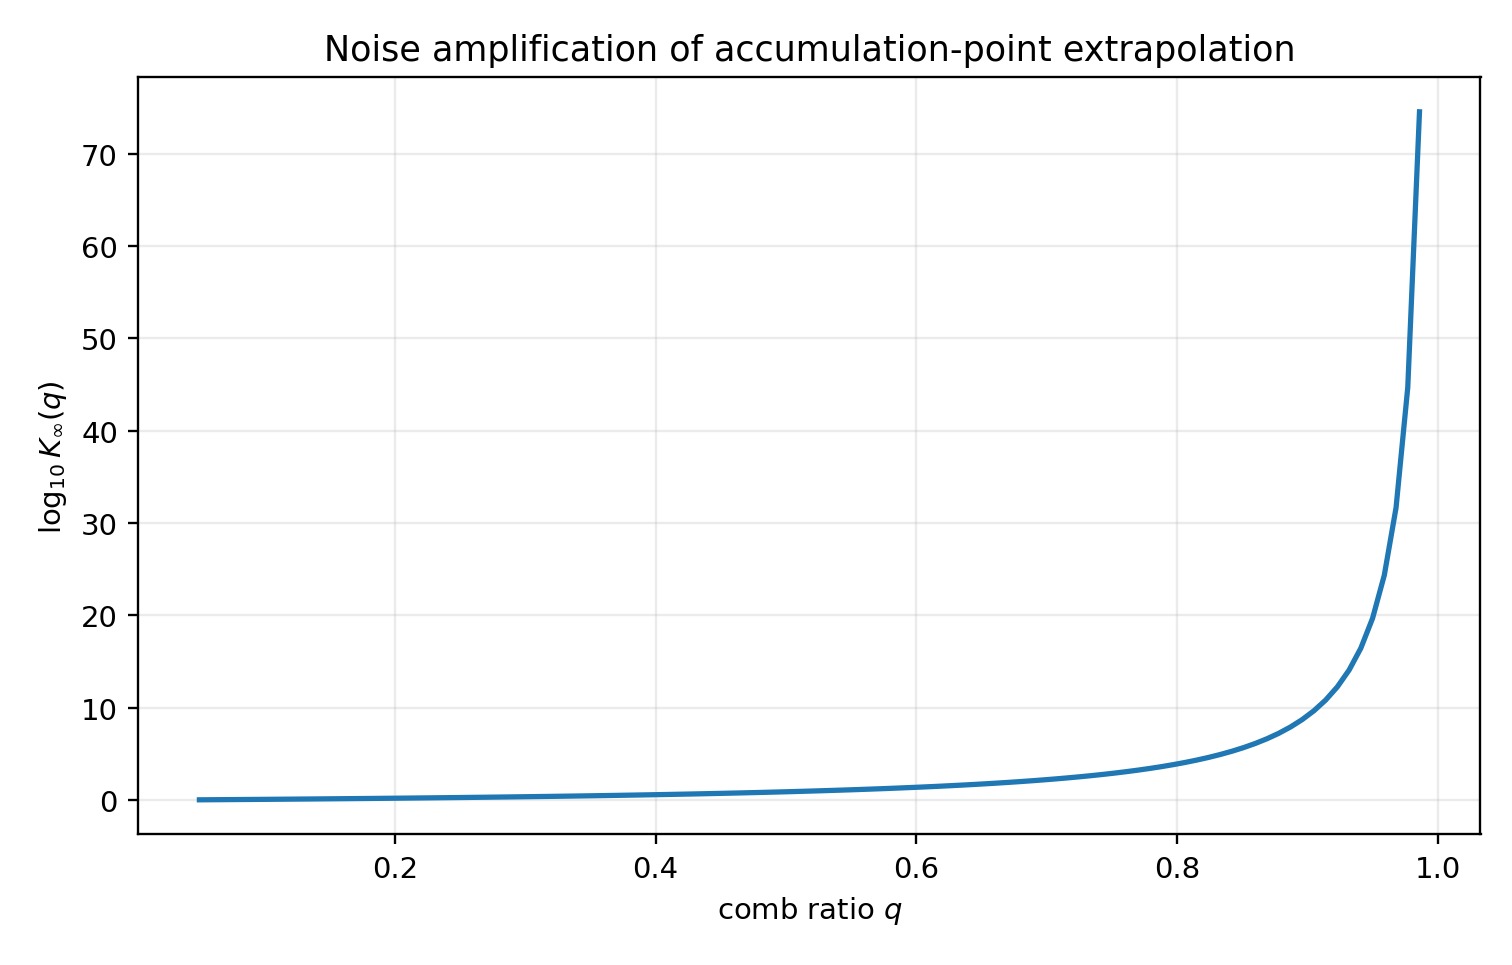
\includegraphics[width=0.88\textwidth]{stability_growth.png}
\caption{The infinite-order total variation
$K_\infty(q)=(-q;q)_\infty/(q;q)_\infty$.  The vertical axis is logarithmic in
base $10$.  Stability is excellent for small and moderate $q$ but deteriorates
nonperturbatively as $q\uparrow1$.}
\label{g1:fig:stability}
\end{figure}

The data file also compares $K_\infty(e^{-t})$ to the asymptotic
\eqref{g1:eq:K-modular}.  For the plotted near-one values the relative difference
is already below the displayed precision, reflecting the exponentially small
modular correction.

\subsection{Regular-variation constants}

\begin{figure}[htbp]
\centering
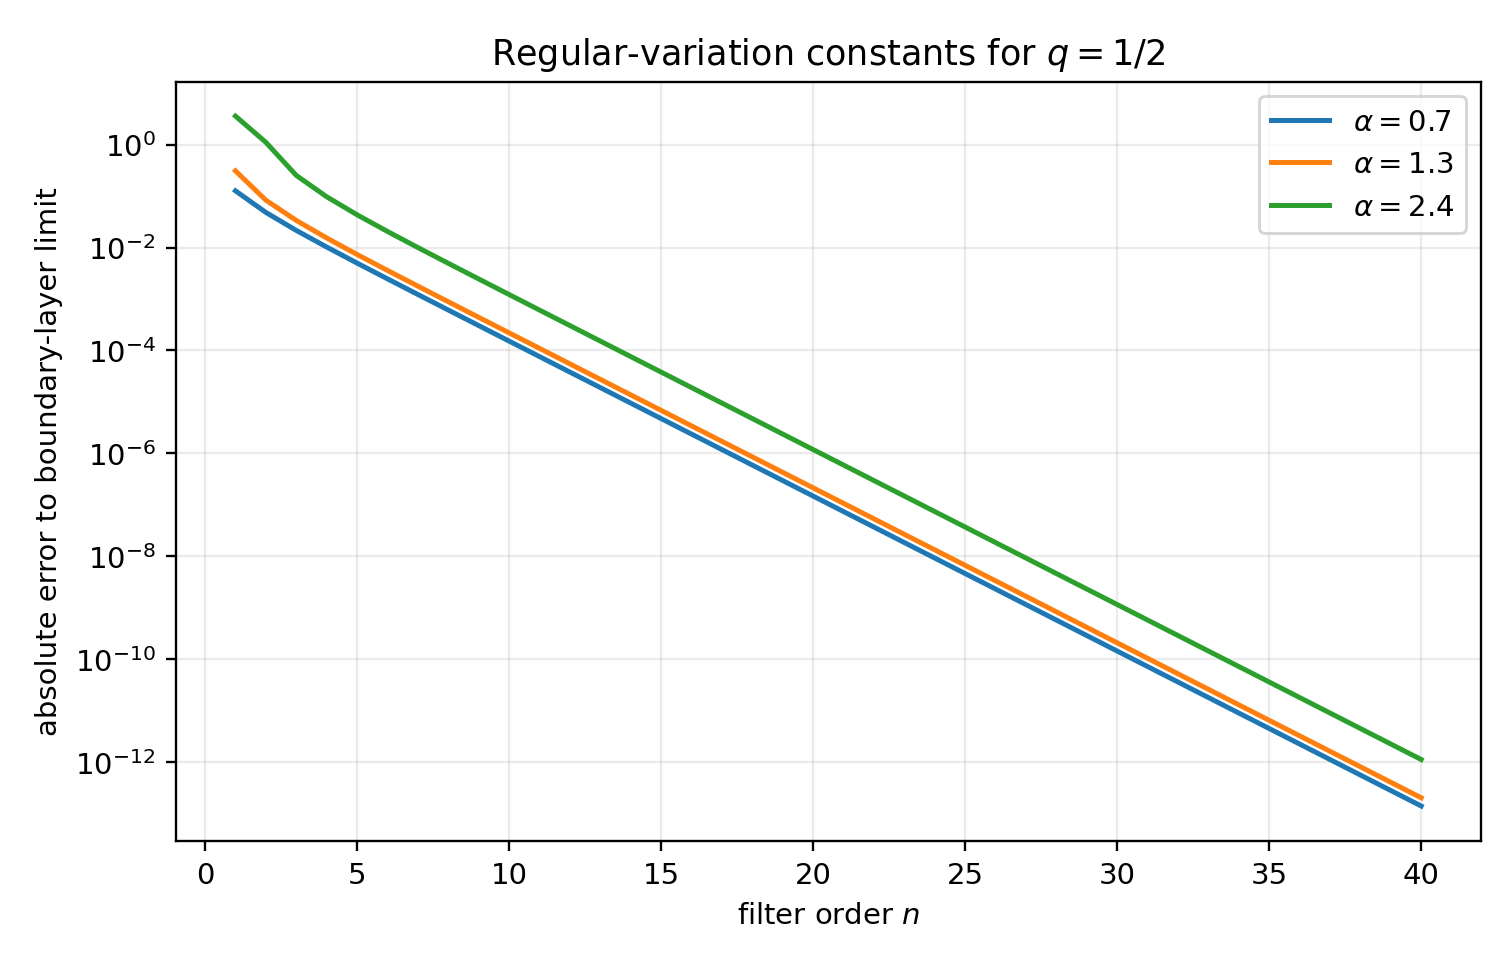
\includegraphics[width=0.88\textwidth]{regular_variation_convergence.png}
\caption{For pure powers $x^\alpha$ at $q=1/2$, the normalized exact multiplier
$(q^{1-\alpha};q)_n/(q;q)_n$ converges geometrically to
$C_q(\alpha)$.  The three exponents illustrate positive and negative limiting
constants.}
\label{g1:fig:regular-variation}
\end{figure}

For example,
\begin{align*}
 C_{1/2}(0.7)&\approx 0.2493175488440439431,\\
 C_{1/2}(1.3)&\approx-0.1538705960439442305,\\
 C_{1/2}(2.4)&\approx 0.2913748265379615867.
\end{align*}
At positive integer exponents the limit is exactly zero, in agreement with
polynomial cancellation.

\subsection{Exact Fabius boundary remainders}

For $A=2^{-(n+1)}$, define
\[
 R_n:=\sum_{k=0}^n\lambda_{n,k}^{(1/2)}F(2^{-(n+1+k)}),
 \qquad
 B_n:=\frac{2^{-n(n+1)}}{(n+1)!}.
\]
The theorem gives $(-1)^nR_n>0$ and $|R_n|/B_n=\Expectation F(S_n)\in(0,1)$.  Exact
fraction arithmetic produces the following decimal summary.

\begin{table}[htbp]
\centering
\caption{Normalized exact dyadic Fabius boundary remainders.}
\label{g1:tab:Fabius-remainders}
\begin{tabular}{rcc}
\toprule
$n$ & sign of $R_n$ & $|R_n|/B_n$\\
\midrule
1  & $-$ & $0.500000000000$\\
2  & $+$ & $0.392067901235$\\
3  & $-$ & $0.285827999336$\\
4  & $+$ & $0.204528650771$\\
5  & $-$ & $0.146778506870$\\
6  & $+$ & $0.106554660592$\\
7  & $-$ & $0.078481279976$\\
8  & $+$ & $0.058671832771$\\
9  & $-$ & $0.044492131277$\\
10 & $+$ & $0.034188031436$\\
\bottomrule
\end{tabular}
\end{table}

\begin{figure}[htbp]
\centering
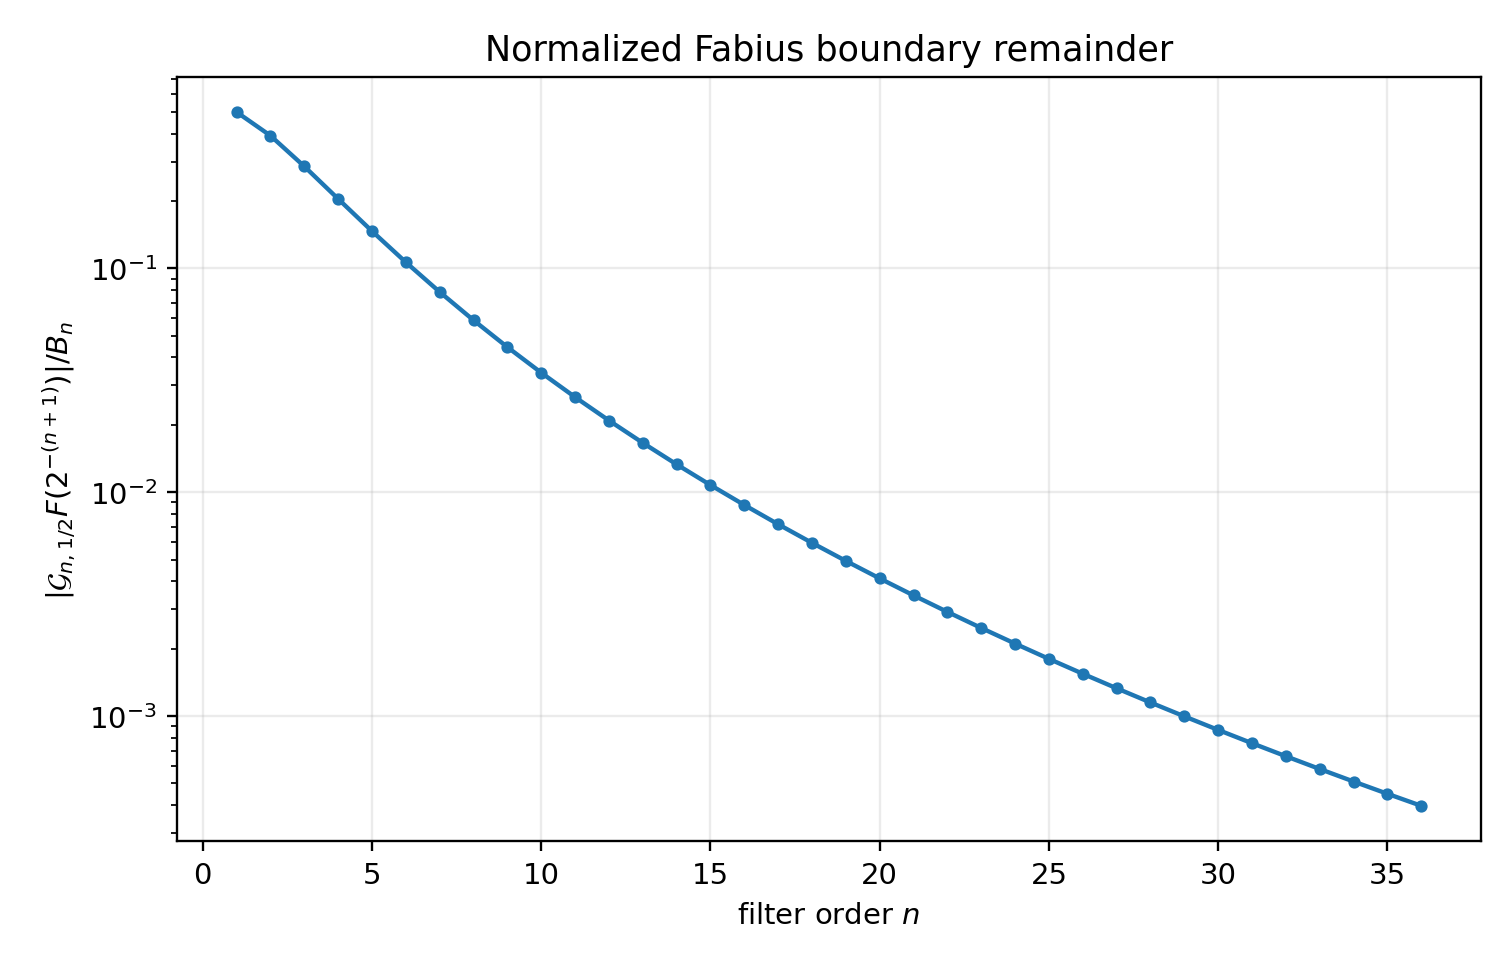
\includegraphics[width=0.88\textwidth]{fabius_boundary_ratio.png}
\caption{The normalized Fabius boundary remainder
$|R_n|/B_n=\Expectation F(S_n)$ through order $36$.  The decrease is much slower than
the already extracted factorial-supergeometric factor $B_n$; its finer
asymptotics are posed as a conjecture in \cref{g1:sec:frontiers}.}
\label{g1:fig:Fabius-ratio}
\end{figure}

\subsection{Reproducibility files}

The script writes four CSV files:
\begin{center}
\begin{tabular}{ll}
\toprule
File & Contents\\
\midrule
\texttt{moment\_checks.csv} & canceled moments and recursion comparison\\
\texttt{stability\_growth.csv} & $K_\infty$, modular approximation, ratio\\
\texttt{regular\_variation.csv} & finite multipliers and limiting constants\\
\texttt{fabius\_boundary.csv} & exact rational filters, bounds, sign checks\\
\bottomrule
\end{tabular}
\end{center}
The archive includes these files and the three PNG figures, so the LaTeX source
can be recompiled without rerunning Python.

\section{Research frontiers and conjectures}
\label{g1:sec:frontiers}

\subsection{A local limit theorem for geometric B-splines}

\cref{g1:eq:Y-scaling-limit} proves weak convergence.  The explicit spline and
limit densities suggest a substantially stronger statement.

\begin{conjecture}[Local density limit]
For every fixed $0<q<1$ and compact interval $K\subset(0,\infty)$,
\begin{equation}
 \sup_{y\in K}
 \left|
 \frac{A}{n+2}B_{n,A,q}\!\left(\frac{Ay}{n+2}\right)-p_q(y)
 \right|\longrightarrow0,
 \label{g1:eq:local-density-conjecture}
\end{equation}
where $p_q$ is given by \eqref{g1:eq:Z-density}.  The convergence should extend to
all derivatives on compact subsets of $(0,\infty)$ after the natural scaling.
\end{conjecture}

A proof might combine the exponential/Dirichlet representation with Fourier or
Laplace inversion and uniform control of the denominator
$(E_*+\cdots+E_n)/(n+2)$.  Such a theorem would turn finite interpolation
kernels into quantitative approximations of a canonical $q$-exponential
density.

\subsection{Fabius--Dirichlet small-value asymptotics}

Let
\[
 \rho_n:=\Expectation F(S_n)=\frac{|R_n|}{B_n}.
\]
The scaling limit $(n+2)S_n\Rightarrow Z_{1/2}$ suggests that $S_n$ is of order
$1/n$, while the Fabius function has a logarithmic-square flatness scale at
zero.  Random fluctuations of $Z_{1/2}$ should affect lower-order terms but not
the leading quadratic logarithm.

\begin{conjecture}[Leading decay of the normalized Fabius remainder]
\begin{equation}
 \log\rho_n
 \sim-\frac{(\log n)^2}{2\log2}
 \qquad(n\to\infty).
 \label{g1:eq:Fabius-rho-conjecture}
\end{equation}
More precisely, the next terms should be obtainable by combining the sharp
Lambert-$W$ endpoint expansion of $F$ developed elsewhere in the ProveIt
project with the density \eqref{g1:eq:Z-density} and a Laplace saddle point.
\end{conjecture}

The experiment in \cref{g1:fig:Fabius-ratio} is consistent with a slowly
converging logarithmic-square law, but orders below $40$ are far too small to
distinguish the lower-order $\log n\log\log n$ and $\log n$ corrections.

\subsection{Second-order regular variation}

\cref{g1:eq:regular-variation} gives only the first boundary-layer limit.  If
$f(x)=x^\alpha L(x)$ and $L$ belongs to a de Haan second-order class, one should
be able to expand
\[
 \frac{(\Gc_{n,q}f)(A)}{f(Aq^n)}
 =C_q(\alpha)+A_1(Aq^n)C_{q,1}(\alpha,\rho)+o(A_1(Aq^n)),
\]
where $A_1$ is the auxiliary function and the correction constant is a
$q$-Mellin moment of the signed boundary layer $\beta_r^{(q)}$.  This would
provide rigorous error estimators for nonanalytic asymptotic extrapolation.

\begin{problem}[Second-order transfer theorem]
Formulate minimal second-order regular-variation hypotheses and compute the
correction constants explicitly from
$(qz;q)_\infty/(q;q)_\infty$.  Treat the resonant integer cases, where
$C_q(\alpha)=0$, separately; there the correction may become the leading term.
\end{problem}

\subsection{The double-scaling transition $q\uparrow1$, $n\to\infty$}

The fixed-order behavior \eqref{g1:eq:fixed-n-q1} and infinite-order behavior
\eqref{g1:eq:K-modular} do not commute.  A natural transition parameter is
$n(1-q)$ or $nt$ when $q=e^{-t}$.

\begin{problem}[Universal transition kernel]
Determine asymptotics of the row polynomial, its total variation, and the
Peano-kernel density when
\[
 n\to\infty,\qquad t\downarrow0,
 \qquad nt\to\tau\in(0,\infty).
\]
One expects a continuum limit connecting geometric-comb extrapolation to
confluent Hermite/Taylor extrapolation at $A$.  The relevant asymptotics should
involve dilogarithms and a saddle point for finite $q$-products.
\end{problem}

\subsection{Optimal filters under analytic priors}

The Gaussian filter is algebraically unique when exactly $n$ integer modes are
canceled with $n+1$ samples.  With more samples than constraints, stability and
bias can be traded.

\begin{problem}[Minimax geometric extrapolation]
Given $M>n$, choose weights on $A,Aq,\ldots,Aq^M$ that preserve constants and
annihilate $x,\ldots,x^n$, while minimizing either total variation or the worst
error over an analytic coefficient-majorant class.  Compare the optimizer with
truncated, damped, and least-squares modifications of $W_{n,q}$.
\end{problem}

The problem is finite-dimensional and convex for total variation, but its
large-$M,n$ structure is likely governed by weighted extremal polynomials on
the spectral set $\{q^m:m\ge0\}$.

\subsection{Inverse Fabius and nonlinear combs}

The inverse Fabius function has endpoint behavior governed by asymptotic
inversion and Lambert $W$, not a regular Taylor series.  A promising strategy is
to choose a nonlinear sample comb $x_k$ so that the dominant inverse asymptotic
modes become geometric in a transformed coordinate.  Confluent modal filters
from \cref{g1:sec:modal} can then remove the leading Lambert-$W$ transseries terms.

\begin{problem}[Lambert-adapted Newton coordinates]
Find a coordinate $u=u(x)$ in which the inverse Fabius germ admits an expansion
in modes $e^{-\alpha u}u^s$, construct the corresponding geometric Newton
series, and determine whether its interpolation coefficients have a positive
kernel or a controlled boundary layer analogous to \eqref{g1:eq:beta}.
\end{problem}

\subsection{Multivariate geometric combs}

Tensor products immediately give interpolation on
$\{A_1q_1^{k_1}\}\times\cdots\times\{A_dq_d^{k_d}\}$, with products of
Gaussian rows.  More interesting are diagonal or simplex combs with a shared
scale index, which interact with multivariate self-similar distributions and
box splines.  The Dirichlet-average interpretation suggests that multivariate
Peano kernels may again have positive probabilistic representations.

\subsection{Formalization boundary and remaining roadmap}

The live Lean corpus has moved beyond a roadmap for the elementary finite
filter.  The modules \nolinkurl{FiniteQBinomialCore.lean},
\nolinkurl{GeometricLagrangeQBinomial.lean},
\nolinkurl{GeometricLagrangeQMoments.lean}, and
\nolinkurl{GeometricLagrangeCompleteHomogeneous.lean} contain named theorems
for finite $q$-products, Gaussian weights, cancellation/residual formulas, the
complete-homogeneous specialization, and the exact finite row norm.
\nolinkurl{LimitConditionNumber.lean} supplies the fixed-$q$ infinite-product
limit, while the geometric-uniform and Rvachev modules named in the opening
status box cover related probability and Fourier infrastructure.

The report-specific obligations that remain are therefore narrower:
\begin{enumerate}[leftmargin=2em]
\item identify geometric divided differences with iterated Jackson derivatives
under explicit field and differentiability hypotheses;
\item construct the infinite Newton series and prove its local uniform
convergence;
\item formalize confluent spectral zeros and the Puiseux--log remainder bound;
\item prove the reversed-row $\ell^1$ limit and the regular-variation transfer;
\item add Hermite--Genocchi/Dirichlet-average infrastructure, the geometric-knot
B-spline moments, and the perpetuity scaling limit;
\item derive the Fabius boundary expectation and the entire scale-reconstruction
theorem from the already formalized finite core.
\end{enumerate}
Until those items exist as checked declarations, the correspondingly labelled
results here remain manuscript theorems.

\section{Complementary Mellin and superflat theory}
\subsection{A target on the same multiplicative line}

A target $x=aq^\alpha$, where $\alpha$ need not be integral, preserves all
$q$-structure.

\begin{theorem}[Arbitrary geometric target]
\label{g2:thm:general-target}
Choose a branch of $q^\alpha$.  If $q^\alpha$ is not one of
$1,q,\ldots,q^n$, then
\begin{equation}
 \ell_{n,j}(aq^\alpha)
 =(-1)^{n-j}q^{\binom{n-j+1}{2}}
 \frac{(q^{\alpha-n};q)_{n+1}}
 {(1-q^{\alpha-j})(q;q)_j(q;q)_{n-j}}.
 \label{g2:eq:general-target-cardinal}
\end{equation}
At $\alpha=j$ the singularity is removable and the value is $1$; at every
other integral node it is $0$.  For $0<q<1$ and
$\Re\alpha\to+\infty$, the weights tend to the zero-target row
\begin{equation}
 \lambda_{n,j}^{(q)}
 =\ell_{n,j}(0)
 =\frac{(-1)^{n-j}q^{\binom{n-j+1}{2}}}
 {(q;q)_j(q;q)_{n-j}}.
 \label{g2:eq:zero-target-row}
\end{equation}
\end{theorem}

\begin{proof}
Use
$\ell_{n,j}(x)=\Omega_{n+1}(x)/((x-aq^j)\Omega'_{n+1}(aq^j))$,
\eqref{gq:eq:nodal-polynomial} and \eqref{gq:eq:barycentric-weight}.  The product
at the target is
\[
 \prod_{r=0}^n(q^\alpha-q^r)
 =(-1)^{n+1}q^{\binom{n+1}{2}}(q^{\alpha-n};q)_{n+1}.
\]
Extracting $-q^j$ from $q^\alpha-q^j$ leaves exactly
\eqref{g2:eq:general-target-cardinal}.  The limiting assertions follow directly
from the product.
\end{proof}

\begin{remark}[$q$-gamma form]
Since
\[
 (q^{\alpha-n};q)_{n+1}
 =(1-q)^{n+1}\frac{\Gamma_q(\alpha+1)}{\Gamma_q(\alpha-n)},
\]
formula \eqref{g2:eq:general-target-cardinal} is meromorphic in $\alpha$ and can
be rewritten entirely with $q$-gamma functions and the $q$-number
$[\alpha-j]_q$.  This is the natural analytic continuation of the cardinal
row, not merely a formal replacement of factorials by $q$-factorials.
\end{remark}


\section{Mellin symbols and exact residuals}
\label{g2:sec:mellin}

\subsection{Complex powers}

The integer moment law in the source monograph is one specialization of a
stronger identity.  Since dilations act diagonally on every chosen branch of
$x^s$, the full spectral response is available at once.

\begin{theorem}[Exact Mellin symbol]
\label{g2:thm:mellin-symbol}
Let $s\in\ComplexNumbers$, choose a branch of $a^s$ and $q^s$, and set
\begin{equation}
 M_{n,q}(s)=\sum_{k=0}^n\lambda_{n,k}^{(q)}q^{ks}.
 \label{g2:eq:mellin-symbol-definition}
\end{equation}
Then
\begin{align}
 M_{n,q}(s)
 &=\frac{\prod_{j=1}^n(q^s-q^j)}{(q;q)_n}
 \label{g2:eq:mellin-product}\\
 &=q^{ns}\frac{(q^{1-s};q)_n}{(q;q)_n}
 \label{g2:eq:mellin-forward}\\
 &=(-1)^nq^{\binom{n+1}{2}}
   \frac{(q^{s-n};q)_n}{(q;q)_n}.
 \label{g2:eq:mellin-reversed}
\end{align}
Equivalently,
\begin{equation}
 (\Gop_{n,q}x^s)(a)=a^sM_{n,q}(s).
 \label{g2:eq:mellin-eigenvalue}
\end{equation}
The zeros at $s=1,\ldots,n$ are simple modulo the imaginary period
$2\pi\ImaginaryUnit/\log q$.
\end{theorem}

\begin{proof}
Evaluate \eqref{g1:eq:row-polynomial} at $z=q^s$.  Factoring $q^s$ from
each factor gives \eqref{g2:eq:mellin-forward}; factoring $-q^j$ gives
\eqref{g2:eq:mellin-reversed}.
\end{proof}

\begin{corollary}[Natural moments and the first residual]
\label{g2:cor:integer-moments}
For $d\in\NaturalNumbers$,
\begin{equation}
 \sum_{k=0}^n\lambda_{n,k}^{(q)}q^{kd}
 =\begin{cases}
 1,&d=0,\\
 0,&1\le d\le n,\\
 (-1)^nq^{\binom{n+1}{2}}\GaussianBinomial{d-1}{n}q,&d\ge n+1.
 \end{cases}
 \label{g2:eq:integer-moment-law}
\end{equation}
\end{corollary}

\begin{proof}
The first two cases follow from the zeros in
\eqref{g2:eq:mellin-product}.  For $d\ge n+1$,
\[
 (q^{d-n};q)_n=\frac{(q;q)_{d-1}}{(q;q)_{d-n-1}},
\]
and substitution into \eqref{g2:eq:mellin-reversed} gives the Gaussian
coefficient.
\end{proof}

\begin{remark}[Fractional endpoint laws]
For fixed $s$ with $\Re s>0$ and $s\notin\NaturalNumbers$,
\begin{equation}
 M_{n,q}(s)
 \sim q^{ns}\frac{(q^{1-s};q)_\infty}{(q;q)_\infty}
 \qquad(n\to\infty).
 \label{g2:eq:fractional-asymptotic}
\end{equation}
Thus a fractional power $x^s$ is not annihilated, but its extrapolation error
has a completely explicit geometric rate.  Integer powers are exceptional
because the finite product terminates at an exact zero.
\end{remark}

\subsection{Logarithmic powers by spectral differentiation}

Differentiate \eqref{g2:eq:mellin-eigenvalue} with respect to $s$.  This gives
closed responses for singular terms common in endpoint asymptotics.

\begin{proposition}[Powers times logarithms]
\label{g2:prop:log-powers}
For every integer $r\ge0$,
\begin{equation}
 \sum_{k=0}^n\lambda_{n,k}^{(q)}(aq^k)^s
 \bigl(\log a+k\log q\bigr)^r
 =\frac{\partial^r}{\partial s^r}\bigl(a^sM_{n,q}(s)\bigr).
 \label{g2:eq:log-power-response}
\end{equation}
In particular, if $1\le d\le n$, then
\begin{equation}
 \sum_{k=0}^n\lambda_{n,k}^{(q)}(aq^k)^d\log(aq^k)
 =a^dM_{n,q}'(d),
 \label{g2:eq:first-log-response}
\end{equation}
where
\begin{equation}
 M_{n,q}'(d)
 =(-1)^{d-1}(\log q)
 q^{d(2n-d+1)/2}
 \frac{(q;q)_{d-1}(q;q)_{n-d}}{(q;q)_n}.
 \label{g2:eq:mellin-derivative-integer}
\end{equation}
\end{proposition}

\begin{proof}
Termwise differentiation is legitimate because the sum is finite.  At
$s=d$, the factor $q^s-q^d$ is the unique vanishing factor in
\eqref{g2:eq:mellin-product}.  Differentiating that factor and splitting the
remaining product below and above $d$ gives
\begin{align*}
 q^d\log q\prod_{\substack{1\le j\le n\\j\ne d}}(q^d-q^j)
 &=(-1)^{d-1}(\log q)
 q^{d(2n-d+1)/2}(q;q)_{d-1}(q;q)_{n-d}.
\end{align*}
Division by $(q;q)_n$ proves \eqref{g2:eq:mellin-derivative-integer}.
\end{proof}

\begin{remark}
A filter that is exact on polynomials need not suppress logarithmic
corrections attached to those powers.  Formula
\eqref{g2:eq:mellin-derivative-integer} quantifies the leakage exactly.  Higher
$s$-derivatives introduce finite sums of $q$-harmonic terms
$(1-q^j)^{-r}$ and can be organized with complete Bell polynomials.
\end{remark}

\subsection{Mellin-transform interpretation}

For a function on $(0,\infty)$ with Mellin transform
\[
 \MellinTransformOf{f}(z)=\int_0^\infty f(x)x^{z-1}\Differential x,
\]
one has
\[
 \MellinTransformOf{f(q^kx)}(z)=q^{-kz}\MellinTransformOf{f}(z).
\]
Hence, on a common strip of convergence,
\begin{equation}
 \MellinTransformOf{\Gop_{n,q}f}(z)=M_{n,q}(-z)\MellinTransformOf{f}(z).
 \label{g2:eq:mellin-transform-multiplier}
\end{equation}
The geometric Lagrange filter is therefore a finite Mellin multiplier.  Its
spectral zeros are the same integer moments that the interpolation formula
annihilates in physical space.  This is the multiplicative analogue of an
ordinary finite-difference stencil whose Fourier symbol has a prescribed zero
at the origin.


\subsection{The limits \texorpdfstring{$q\to1$}{q to 1} and \texorpdfstring{$q\to0$}{q to 0}}

\begin{proposition}[Taylor limit]
\label{g2:prop:taylor-limit}
For fixed $k$, as $q\to1$,
\[
 D_q^kf(a)\longrightarrow f^{(k)}(a),
 \qquad [k]_q!\longrightarrow k!,
 \qquad \Phi_k(x)\longrightarrow(x-a)^k.
\]
Thus \eqref{gq:eq:q-taylor-interpolant} tends termwise to the ordinary Taylor
polynomial about $a$.
\end{proposition}

\begin{proof}
The first statement follows by repeated use of the standard Jackson derivative
limit on a sufficiently differentiable function; the other two are immediate
from their finite products.
\end{proof}

At the opposite endpoint, $D_0f(x)=(f(x)-f(0))/x$ is a tail-quotient operator.
For $f(x)=\sum c_mx^m$,
\[
 \lim_{q\to0}\frac{D_q^kf(a)}{[k]_q!}
 =\sum_{r\ge0}c_{k+r}a^r,
 \qquad
 \lim_{q\to0}\Phi_k(x)=
 \begin{cases}
 1,&k=0,\\
 (x-a)x^{k-1},&k\ge1.
 \end{cases}
\]
The limiting expansion telescopes.  It is not Hermite interpolation at a
multiple node: the geometric rates retain ordered information about how the
nodes approach zero.  A genuine confluent theory requires a further
renormalization and is listed as \Cref{g2:prob:q0-confluent}.

\subsection{Neville, Richardson, and Romberg recurrences}

\begin{theorem}[Geometric Neville recurrence]
\label{g2:thm:neville}
For $i,m\ge0$, let $P_{i,m}$ be the interpolant characterized by
\[
 P_{i,m}(aq^{i+r})=f(aq^{i+r})\qquad(0\le r\le m).
\]
Then
\begin{equation}
 P_{i,m}(x)=
 \frac{(x-aq^{i+m})P_{i,m-1}(x)
      -(x-aq^i)P_{i+1,m-1}(x)}
      {aq^i-aq^{i+m}}.
 \label{g2:eq:geometric-neville}
\end{equation}
At $x=0$, with $R_i^{(0)}=f(aq^i)$,
\begin{equation}
 R_i^{(m)}
 =\frac{R_{i+1}^{(m-1)}-q^mR_i^{(m-1)}}{1-q^m},
 \qquad
 R_0^{(n)}=(\Gop_{n,q}f)(a).
 \label{g2:eq:richardson-recurrence}
\end{equation}
\end{theorem}

\begin{proof}
The numerator in \eqref{g2:eq:geometric-neville} has degree at most $m$ and takes
the required values at both endpoint nodes and all shared interior nodes;
uniqueness proves the formula.  Substitute $x=0$ and cancel $aq^i$.
\end{proof}

\begin{corollary}[Generalized Richardson cancellation]
\label{g2:cor:richardson}
Suppose approximations at scales $h_i=h_0r^i$ have an expansion
\[
 T(h)=L+c_1h^\rho+c_2h^{2\rho}+\cdots.
\]
Apply \eqref{g2:eq:richardson-recurrence} with $q=r^\rho$ to the data $T(h_i)$.
After $n$ levels, the first $n$ error powers are annihilated exactly.  Romberg
quadrature is the special case in which the trapezoidal error uses even powers
and hence $q=r^2$.
\end{corollary}

\begin{proof}
The recurrence is the degree-$n$ interpolation functional at the point
$0$ on nodes $1,q,\ldots,q^n$.  It fixes the constant mode and annihilates
$q^{ki}$ for $1\le k\le n$, equivalently the error modes
$h^{k\rho}$.  Linearity therefore removes the first $n$ displayed error
powers.  For the trapezoidal expansion only even powers occur, so replacing
$r$ by $r^2$ gives the Romberg case.
\end{proof}

\begin{remark}
This recurrence is often numerically preferable to forming the closed weights.
It also explains the historical term ``deferred approach to the limit'': each
new level eliminates one Mellin eigenmode of the asymptotic error.
\end{remark}


\section{Convergence at an accumulation point and divergence away from it}
\label{g2:sec:superflat}

\subsection{The zero row is a regular summability method}

\begin{theorem}[Regularity at the accumulation point]
\label{g2:thm:regular-summability}
Let $0<q<1$ and let $y_k\to L$.  Then
\begin{equation}
 \sum_{k=0}^n\lambda_{n,k}^{(q)}y_k\longrightarrow L.
 \label{g2:eq:regular-summability}
\end{equation}
Equivalently, if $f$ is continuous at $0$, the interpolating polynomial through
$(aq^k,f(aq^k))$, $0\le k\le n$, satisfies
\begin{equation}
 (\Iop_nf)(0)\longrightarrow f(0).
 \label{g2:eq:continuous-zero-convergence}
\end{equation}
\end{theorem}

\begin{proof}
The rows reproduce constants by \eqref{g2:eq:integer-moment-law}; their
$\ell^1$ norms are bounded by $K(q)$ by \Cref{g1:thm:row-norm}; and for each fixed
$k$,
\[
 |\lambda_{n,k}^{(q)}|
 =\frac{q^{\binom{n-k+1}{2}}}
 {(q;q)_k(q;q)_{n-k}}\longrightarrow0.
\]
These are precisely the Toeplitz regularity conditions.  For completeness,
subtract $L$, split the sum at a fixed $K$, make the tail small using the
bounded row norm, and then let $n\to\infty$ in the finite head.
\end{proof}

\subsection{The limiting profile viewed from the finest tooth}

Reindex the row by $r=n-k$.  For each fixed $r$,
\begin{equation}
 \lambda_{n,n-r}^{(q)}
 \longrightarrow
 \mu_r^{(q)}
 :=\frac{(-1)^rq^{\binom{r+1}{2}}}
 {(q;q)_\infty(q;q)_r}.
 \label{g2:eq:limiting-row-profile}
\end{equation}
Euler's infinite theorem gives the generating function
\begin{equation}
 \sum_{r=0}^\infty\mu_r^{(q)}z^r
 =\frac{(qz;q)_\infty}{(q;q)_\infty},
 \qquad
 \sum_{r=0}^\infty\mu_r^{(q)}=1.
 \label{g2:eq:limiting-profile-generating}
\end{equation}
Thus the mass does not remain attached to any fixed physical node; it travels
with the finest scale $aq^n$ and approaches a signed, absolutely summable
profile in the reversed index.  This is the mechanism behind
\Cref{g2:thm:regular-summability}.

\subsection{Power, Puiseux, and logarithmic endpoint expansions}

Suppose a germ has a convergent or asymptotic expansion
\[
 f(x)=L+\sum_{r}c_rx^{\alpha_r}(\log x)^{m_r},
 \qquad \Re\alpha_r>0.
\]
Theorems \ref{g2:thm:mellin-symbol} and \ref{g2:prop:log-powers} give the filter of
each term exactly.  In particular, a nonintegral leading exponent $\alpha$
produces the rate $q^{n\alpha}$ times an explicit $q$-product, while an
integral polynomial jet is deleted once $n$ reaches its degree.  The filter is
therefore an endpoint asymptotic microscope: its decay rate distinguishes
fractional regularity from an analytic integer jet.

\begin{proposition}[A simple Hölder estimate]
\label{g2:prop:holder-filter}
If $|f(x)-f(0)|\le C|x|^\alpha$ on the comb, with $\alpha>0$, then
\begin{equation}
 |(\Gop_{n,q}f)(a)-f(0)|
 \le C|a|^\alpha
 \sum_{k=0}^n|\lambda_{n,k}^{(q)}|q^{k\alpha}.
 \label{g2:eq:holder-bound}
\end{equation}
For fixed $q$ and $\alpha$, the right side is $O(q^{n\alpha})$.
\end{proposition}

\begin{proof}
The first statement is the triangle inequality.  Reindex $r=n-k$.  Since
$(q;q)_m\ge(q;q)_\infty$ for every $m$, one has
\begin{align*}
 q^{-n\alpha}
 \sum_{k=0}^n|\lambda_{n,k}^{(q)}|q^{k\alpha}
 &=\sum_{r=0}^n
 \frac{q^{\binom{r+1}{2}-r\alpha}}
 {(q;q)_{n-r}(q;q)_r}\\
 &\le \frac1{(q;q)_\infty^2}
 \sum_{r=0}^\infty q^{\binom{r+1}{2}-r\alpha}<\infty.
\end{align*}
The last series converges for every fixed $\alpha$ because its exponent is
quadratic in $r$.  This uniform bound proves the stated $O(q^{n\alpha})$
estimate.  Dominated convergence also gives the sharper limit
\[
 q^{-n\alpha}
 \sum_{k=0}^n|\lambda_{n,k}^{(q)}|q^{k\alpha}
 \longrightarrow
 \sum_{r=0}^\infty|\mu_r^{(q)}|q^{-r\alpha}.
\]
\end{proof}

\subsection{Superflat data force divergence off the comb}

The favorable result at $0$ has a nearly opposite counterpart everywhere
else.  It is useful to formulate it directly for data, without assuming that
they initially came from a function.

\begin{definition}
A sequence $y_j\to L$ is \emph{$q$-superflat at its limit} if
\begin{equation}
 y_j-L=o(q^{mj})\qquad(j\to\infty)
 \label{g2:eq:q-superflat}
\end{equation}
for every $m\in\NaturalNumbers$.
\end{definition}

\begin{theorem}[Exact convergence set for nontrivial superflat data]
\label{g2:thm:superflat-divergence}
Let $0<q<1$, $a\ne0$, and let $y_j\to L$ be $q$-superflat.  Assume
$y_j\ne L$ for infinitely many $j$.  Let
\begin{equation}
 P_n(x)=\sum_{k=0}^n A_k\Phi_k(x)
 \label{g2:eq:superflat-newton}
\end{equation}
be the polynomial interpolating $P_n(aq^j)=y_j$ for $0\le j\le n$.  Then
\begin{equation}
 \limsup_{k\to\infty}|A_k|^{1/k}=\infty.
 \label{g2:eq:superexponential-A}
\end{equation}
Moreover:
\begin{enumerate}
\item $P_n(0)\to L$;
\item for each $m\ge0$, $P_n(aq^m)=y_m$ once $n\ge m$;
\item for every $x\in\ComplexNumbers\setminus(\{0\}\cup\{aq^m:m\ge0\})$, the increments
      $A_n\Phi_n(x)$ fail to tend to zero, and the sequence $P_n(x)$ diverges;
      indeed it is unbounded along a subsequence.
\end{enumerate}
Thus the convergence set is exactly the geometric comb together with its
accumulation point.
\end{theorem}

\begin{proof}
Subtract $L$; this changes only $A_0$ and reduces to $L=0$.  Suppose, contrary
to \eqref{g2:eq:superexponential-A}, that $|A_k|\le CR^{-k}$ for some $R>0$.
For every $0<r<R$, the estimate
\[
 \sup_{|z|\le r}|\Phi_k(z)|
 \le r^k\prod_{j=0}^\infty(1+|a|q^j/r)
\]
shows that $g(z)=\sum_{k\ge0}A_k\Phi_k(z)$ is analytic on $|z|<R$.
For every sufficiently large $j$, $|aq^j|<R$, and all terms with $k>j$
vanish at $aq^j$.  Hence
\[
 g(aq^j)=P_j(aq^j)=y_j.
\]
If the first nonzero Taylor coefficient of $g$ at $0$ had order $m$, then
$g(aq^j)/(aq^j)^m$ would tend to a nonzero constant.  This contradicts
$q$-superflatness.  Therefore every Taylor coefficient vanishes, so $g$ is
identically zero near $0$, contradicting the assumption that infinitely many
$y_j$ are nonzero.  This proves \eqref{g2:eq:superexponential-A}.

Assertion 1 is \Cref{g2:thm:regular-summability}, and assertion 2 is interpolation.
For a point $x$ in assertion 3,
\begin{equation}
 \Phi_n(x)=x^n\prod_{r=0}^{n-1}\left(1-\frac{aq^r}{x}\right).
 \label{g2:eq:basis-fixed-x}
\end{equation}
The infinite product tends to $(a/x;q)_\infty\ne0$, because $x$ is not a
node.  Hence $|\Phi_n(x)|^{1/n}\to|x|>0$.  Together with
\eqref{g2:eq:superexponential-A}, this implies
\(
 \limsup|A_n\Phi_n(x)|^{1/n}=\infty
\); the increments do not tend to zero.  Finally,
$|P_n-P_{n-1}|=|A_n\Phi_n|$ is unbounded along a subsequence, so at least one
of each adjacent pair $P_n,P_{n-1}$ is unbounded along a subsequence.
\end{proof}

\begin{remark}[A precise geometric Runge phenomenon]
This is not the classical Runge phenomenon caused by equispaced nodes on a
fixed interval.  The comb is not dense away from $0$.  Superflat nonzero data
cannot be the trace of a nonzero analytic germ at the accumulation point;
the interpolation coefficients must therefore leave every exponential class.
The instability is an analytic-continuation obstruction encoded in a
Vandermonde problem.
\end{remark}

\begin{remark}[Derivative-enhanced interpolation]
Adding finitely many Hermite conditions at any fixed collection of nonzero
teeth does not remove the obstruction: an exponentially bounded coefficient
sequence would still define an analytic germ with a superflat nonzero trace.
A successful regularization must either change the approximation space, use a
number of derivative conditions growing with $n$, or explicitly build
flatness into the basis.  Rvachev atoms are natural candidates for the last
option.
\end{remark}


\section{The geometric-uniform family}
\label{g2:sec:geometric-uniform}

\subsection{Probability law, support, and refinement}

Let $U_0,U_1,\ldots$ be independent uniform random variables on $[0,1]$ and
set
\begin{equation}
 X_q=(1-q)\sum_{j=0}^\infty q^jU_j,
 \qquad 0<q<1.
 \label{g2:eq:Xq-definition}
\end{equation}
This is a geometric member of the infinite-convolution class studied by
Jessen and Wintner~\cite{JessenWintner1935}.  The coefficients are positive
and sum to $1$, so $0\le X_q\le1$.  Reflection
of every $U_j$ shows
\begin{equation}
 X_q\stackrel d=1-X_q.
 \label{g2:eq:Xq-symmetry}
\end{equation}
Let $F_q(x)=\Probability(X_q\le x)$, extended by $0$ to $x\le0$ and by $1$ to
$x\ge1$.  Removing the first coordinate gives the affine fixed-point law
\begin{equation}
 X_q\stackrel d=(1-q)U+qX_q',
 \label{g2:eq:Xq-fixed-point}
\end{equation}
where $X_q'$ is an independent copy.  Consequently
\begin{align}
 F_q(x)
 &=\int_0^1F_q\!\left(\frac{x-(1-q)u}{q}\right)\Differential u
 \label{g2:eq:Fq-integral-equation}\\
 &=\frac q{1-q}
 \int_{(x-(1-q))/q}^{x/q}F_q(t)\Differential t.
 \label{g2:eq:Fq-integral-equation-2}
\end{align}
Differentiation gives
\begin{equation}
 F_q'(x)=\frac{F_q(x/q)-F_q((x-(1-q))/q)}{1-q}.
 \label{g2:eq:Fq-derivative}
\end{equation}

\begin{proposition}[Smooth compactly supported density]
\label{g2:prop:uq-smooth}
The centered random variable
\begin{equation}
 Z_q=2X_q-1=(1-q)\sum_{j=0}^\infty q^jV_j,
 \qquad V_j\sim\operatorname{Unif}[-1,1],
 \label{g2:eq:Zq-definition}
\end{equation}
has an even $C^\infty$ density $u_q$ supported on $[-1,1]$.  With the Fourier
convention
$\FourierTwoPi{f}(\xi)=\int_\RealNumbers f(x)\EulerE^{-2\pi\ImaginaryUnit\xi x}\Differential x$,
\begin{equation}
 \FourierTwoPi{u_q}(\xi)=\prod_{j=0}^\infty
 \SincPi\!\left(2(1-q)q^j\xi\right),
 \qquad
 \SincPi(t)=\frac{\sin(\pi t)}{\pi t}.
 \label{g2:eq:uq-fourier-product}
\end{equation}
Moreover
\begin{equation}
 u_q(z)=\frac12F_q'\!\left(\frac{z+1}{2}\right).
 \label{g2:eq:uq-Fq-relation}
\end{equation}
\end{proposition}

\begin{proof}
The characteristic function factors by independence and gives
\eqref{g2:eq:uq-fourier-product}.  To see rapid decay, use
$|\SincPi(t)|\le\min(1,1/(\pi|t|))$ on the first
$N\asymp\log|\xi|/|\log q|$ factors.  The logarithm of the resulting product
is $-c_q(\log|\xi|)^2+O_q(\log|\xi|)$, hence the product decreases faster than
any inverse power.  Fourier inversion then gives a $C^\infty$ density.  The
support and evenness follow from \eqref{g2:eq:Zq-definition}; the density change
of variables gives \eqref{g2:eq:uq-Fq-relation}.
\end{proof}

\begin{remark}
The repository's formal development treats a still broader geometric-uniform
law, including negative ratios and uniqueness of the affine distributional
fixed point.  The positive-ratio case above is the one naturally matched to a
one-sided interpolation comb.
\end{remark}

\subsection{Moments and Bernoulli cumulants}

Write
\begin{equation}
 \mu_n(q)=\Expectation X_q^n.
 \label{g2:eq:muq-definition}
\end{equation}

\begin{theorem}[Moment recurrence]
\label{g2:thm:moment-recurrence}
The moments satisfy $\mu_0(q)=1$ and, for $n\ge1$,
\begin{equation}
 (1-q^n)\mu_n(q)
 =\sum_{k=0}^{n-1}\binom nk
 q^k(1-q)^{n-k}\frac{\mu_k(q)}{n-k+1}.
 \label{g2:eq:general-moment-recurrence}
\end{equation}
At $q=1/2$ this reduces to
\begin{equation}
 (2^n-1)\mu_n(1/2)
 =\sum_{k=0}^{n-1}\binom nk\frac{\mu_k(1/2)}{n-k+1}.
 \label{g2:eq:dyadic-moment-recurrence}
\end{equation}
\end{theorem}

\begin{proof}
Raise \eqref{g2:eq:Xq-fixed-point} to the $n$th power, expand, and use
$\Expectation U^r=1/(r+1)$.  Move the $k=n$ term to the left.  At $q=1/2$ every factor
$q^k(1-q)^{n-k}$ equals $2^{-n}$, and multiplication by $2^n$ gives
\eqref{g2:eq:dyadic-moment-recurrence}.
\end{proof}

The centered moment generating function is
\begin{equation}
 \Mq(z)=\Expectation\EulerE^{zZ_q}
 =\prod_{j=0}^\infty
 \frac{\sinh((1-q)q^jz)}{(1-q)q^jz}.
 \label{g2:eq:uq-mgf}
\end{equation}
Using
\[
 \log\frac{\sinh z}{z}
 =\sum_{m\ge1}\frac{2^{2m-1}B_{2m}}{m(2m)!}z^{2m},
\]
we obtain the even cumulants
\begin{equation}
 \kappa_{2m}(Z_q)
 =\frac{2^{2m}B_{2m}}{2m}
   \frac{(1-q)^{2m}}{1-q^{2m}},
 \qquad
 \kappa_{2m+1}(Z_q)=0.
 \label{g2:eq:uq-cumulants}
\end{equation}
Thus the same geometric series that produces the interpolation denominators
also produces the cumulant denominators.  At $q=1/2$,
\begin{equation}
 \kappa_{2m}(Z_{1/2})
 =\frac{B_{2m}}{2m(1-4^{-m})}.
 \label{g2:eq:up-cumulants}
\end{equation}
Moments can be recovered from these cumulants by complete Bell polynomials,
providing a second exact route parallel to \eqref{g2:eq:dyadic-moment-recurrence}.

\subsection{The left boundary layer}

For $0\le x\le1-q$, the second term in \eqref{g2:eq:Fq-derivative} vanishes, so
\begin{equation}
 F_q'(x)=\frac1{1-q}F_q(x/q).
 \label{g2:eq:left-boundary-first}
\end{equation}
Iteration gives the geometric derivative tower.

\begin{lemma}[Boundary derivative tower]
\label{g2:lem:boundary-tower}
If $m\ge1$ and $0\le x\le(1-q)q^{m-1}$, then
\begin{equation}
 F_q^{(m)}(x)
 =(1-q)^{-m}q^{-\binom m2}F_q(x/q^m).
 \label{g2:eq:boundary-derivative-tower}
\end{equation}
\end{lemma}

\begin{proof}
Induct on $m$.  The case $m=1$ is
\eqref{g2:eq:left-boundary-first}.  Differentiating the induction hypothesis
contributes a factor $q^{-1}$, and the domain assumption ensures that the next
use of \eqref{g2:eq:left-boundary-first} remains in the left boundary layer.
\end{proof}

\subsection{Comb samples are normalized moments}

The ratio $q=1/2$ is geometrically critical: the first uniform block has
length $1-q$, while the tail has length $q$, and these are equal exactly at
$q=1/2$.  For every $q\le1/2$, however, the tooth $q^n$ still lies inside the
$n$th iterated boundary layer, which is enough for the following formula.

\begin{theorem}[Geometric comb--moment identity]
\label{g2:thm:comb-moment}
For $0<q\le1/2$ and every $n\ge0$,
\begin{equation}
 F_q(q^n)
 =\frac{q^{\binom{n+1}{2}}}{(1-q)^n n!}\,\mu_n(q).
 \label{g2:eq:comb-moment}
\end{equation}
\end{theorem}

\begin{proof}
The case $n=0$ is $F_q(1)=1$.  For $n\ge1$, compact support and smoothness
imply that $F_q$ and all its derivatives vanish at $0$.  Since
$q^n\le(1-q)q^{n-1}$ when $q\le1/2$, Taylor's integral formula and
\Cref{g2:lem:boundary-tower} give
\begin{align*}
 F_q(q^n)
 &=\frac1{(n-1)!}\int_0^{q^n}(q^n-t)^{n-1}F_q^{(n)}(t)\Differential t\\
 &=\frac{(1-q)^{-n}q^{-\binom n2}}{(n-1)!}
   \int_0^{q^n}(q^n-t)^{n-1}F_q(t/q^n)\Differential t\\
 &=\frac{q^{n^2-\binom n2}}{(1-q)^n(n-1)!}
   \int_0^1(1-u)^{n-1}F_q(u)\Differential u.
\end{align*}
By Fubini,
\[
 \int_0^1(1-u)^{n-1}F_q(u)\Differential u
 =\frac1n\Expectation(1-X_q)^n.
\]
Symmetry \eqref{g2:eq:Xq-symmetry} changes the last moment to $\mu_n(q)$, and
$n^2-\binom n2=\binom{n+1}{2}$.
\end{proof}

\begin{remark}[What fails for $q>1/2$]
The formula is not expected to survive unchanged.  The point $q^n$ lies beyond
the pure left boundary layer, so the reflected term in
\eqref{g2:eq:Fq-derivative} enters before the $n$th differentiation.  The
resulting correction should be indexed by affine words recording boundary
crossings.  Deriving a closed word-sum or automaton formula is
\Cref{g2:prob:qgt-half}.
\end{remark}

\subsection{The classical Fabius and Rvachev normalizations}

Put
\[
 F=F_{1/2},\qquad X=X_{1/2},\qquad u=u_{1/2}.
\]
Then $F$ is the bounded Fabius function.  On $0\le x\le1/2$,
\[
 F'(x)=2F(2x),
 \qquad
 F(1-x)=1-F(x).
\]
The centered density $u$ is Rvachev's up-function in the probability
normalization.  From \eqref{g2:eq:uq-Fq-relation},
\begin{equation}
 u(z)=
 \begin{cases}
 F(z+1),&-1\le z\le0,\\
 F(1-z),&0\le z\le1,\\
 0,&|z|\ge1.
 \end{cases}
 \label{g2:eq:up-Fabius-piecewise}
\end{equation}
Its Fourier transform is the canonical infinite sinc product
\begin{equation}
 \FourierTwoPi{u}(\xi)=\prod_{j=0}^\infty\SincPi(\xi/2^j).
 \label{g2:eq:up-fourier-classical}
\end{equation}
The construction and these identities agree with the classical treatments of
Fabius~\cite{Fabius1966} and Arias de Reyna~\cite{Arias2017Definition}, and
with the normalization used in the repository's primary exposition
\cite{ProveItFabius}.

Write $\mu_n:=\mu_n(1/2)$ and introduce the Mersenne product
\begin{equation}
 \mathfrak M_n:=\prod_{r=1}^n(2^r-1),
 \qquad \mathfrak M_0:=1.
 \label{g2:eq:mersenne-definition}
\end{equation}

\begin{proposition}[Mersenne form of the dyadic origin row]
\label{g2:prop:dyadic-mersenne-row}
For every $n\ge0$,
\begin{align}
 (1/2;1/2)_n
 &=2^{-\binom{n+1}{2}}\mathfrak M_n,
 \label{g2:eq:qpoch-mersenne}\\
 \lambda_{n,k}^{(1/2)}
 &=(-1)^{n-k}{2^{\binom{k+1}{2}}
 \over\mathfrak M_k\mathfrak M_{n-k}}
 \qquad(0\le k\le n).
 \label{g2:eq:dyadic-lambda-mersenne}
\end{align}
\end{proposition}

\begin{proof}
In the Pochhammer product, write
$1-2^{-r}=2^{-r}(2^r-1)$ and multiply the powers $2^{-r}$ for
$1\le r\le n$.  Substitution of that identity at $k$ and $n-k$ into
\eqref{g1:eq:lambda} cancels the remaining powers of two and yields the
second formula.
\end{proof}


\subsection{The endpoint extrapolant as a Mersenne--moment convolution}

Let $P_n$ interpolate $F$ at
$1,1/2,\ldots,2^{-n}$ and put $E_n=P_n(0)$.

\begin{theorem}[Exact endpoint convolution]
\label{g2:thm:fabius-endpoint-convolution}
For every $n\ge0$,
\begin{equation}
 E_n
 =\sum_{k=0}^n(-1)^{n-k}
 \frac{2^k\mu_k}
 {k!\,\mathfrak M_k\mathfrak M_{n-k}}.
 \label{g2:eq:fabius-endpoint-convolution}
\end{equation}
The first values are
\[
 1,\quad 0,\quad -\frac{13}{27},\quad \frac19,\quad
 \frac{4418}{637875},\quad -\frac{3218}{1318275},\ldots.
\]
Despite the initially nonmonotone behavior, $E_n\to0$.
\end{theorem}

\begin{proof}
Substitute \eqref{gq:eq:fabius-inverse-dyadic} and
\eqref{g2:eq:dyadic-lambda-mersenne} into
$E_n=\sum_k\lambda_{n,k}^{(1/2)}F(2^{-k})$.  The powers combine as
$2^{\binom{k+1}{2}-\binom k2}=2^k$.  Convergence follows independently from
\Cref{g2:thm:regular-summability}.
\end{proof}

The same mechanism yields a quantitative bound throughout the
geometric-uniform family.

\begin{theorem}[Quadratic endpoint bound]
\label{g2:thm:quadratic-endpoint-bound}
Let $0<q\le1/2$, and let $P_{n,q}$ interpolate $F_q$ at
$1,q,\ldots,q^n$.  Then
\begin{equation}
 |P_{n,q}(0)|
 \le
 \frac{\exp((1-q)^{-1})}{(q;q)_\infty^2}
 q^{\binom{n+1}{2}-\Floor{n^2/4}}.
 \label{g2:eq:quadratic-endpoint-bound}
\end{equation}
In particular the convergence is at least as fast as
$q^{n^2/4+O(n)}$, and hence faster than every fixed geometric rate.
\end{theorem}

\begin{proof}
Use the exact sample formula \eqref{g2:eq:comb-moment}, the bound
$0\le\mu_k(q)\le1$, and \eqref{g2:eq:zero-target-row}:
\begin{align*}
 |P_{n,q}(0)|
 &\le\sum_{k=0}^n
 \frac{q^{\binom{n-k+1}{2}+\binom{k+1}{2}}}
 {(q;q)_k(q;q)_{n-k}}
 \frac{(1-q)^{-k}}{k!}.
\end{align*}
The exponent is
\[
 \binom{n+1}{2}-k(n-k)
 \ge\binom{n+1}{2}-\Floor{n^2/4}.
\]
Also $(q;q)_k,(q;q)_{n-k}\ge(q;q)_\infty$.  Extract the smallest power of
$q$ and majorize the remaining sum by
$\sum_{k\ge0}(1-q)^{-k}/k!=\exp((1-q)^{-1})$.
\end{proof}

\subsection{Newton coefficients as a Gaussian moment transform}

Write the Newton form
\begin{equation}
 P_n(x)=\sum_{k=0}^n A_k\prod_{r=0}^{k-1}(x-2^{-r}).
 \label{g2:eq:fabius-newton-form}
\end{equation}
The coefficient $A_k$ is independent of the final interpolation degree once
the first $k+1$ nodes are present.

\begin{theorem}[General geometric-uniform moment transform]
\label{g2:thm:general-moment-transform}
For $0<q\le1/2$, let $A_n(q)$ be the Newton coefficient for the data
$F_q(1),F_q(q),\ldots$.  Then
\begin{equation}
 A_n(q)=\frac1{(q;q)_n}
 \sum_{j=0}^n(-1)^j
 \GaussianBinomial nj{q^{-1}}
 \left(\frac q{1-q}\right)^j
 \frac{\mu_j(q)}{j!}.
 \label{g2:eq:general-Gaussian-moment-transform}
\end{equation}
The transform is triangular and invertible.  If
$B_k=(q;q)_kA_k(q)$ and $Q=q^{-1}$, then
\begin{equation}
 \frac{\mu_n(q)}{n!}
 =\left(\frac{1-q}{q}\right)^n
 \sum_{k=0}^n(-1)^kQ^{\binom{n-k}{2}}
 \GaussianBinomial nkQ B_k.
 \label{g2:eq:inverse-Gaussian-moment-transform}
\end{equation}
\end{theorem}

\begin{proof}
Insert \eqref{g2:eq:comb-moment} into the explicit divided difference
\eqref{gq:eq:geometric-divided-difference} with $c=1$.  The powers simplify by
\[
 q^{-jn+\binom{j+1}{2}+\binom{j+1}{2}}(1-q)^{-j}
 =q^{-j(n-j)}\left(\frac q{1-q}\right)^j,
\]
and reciprocity
$q^{-j(n-j)}\GaussianBinomial njq=\GaussianBinomial nj{q^{-1}}$ proves
\eqref{g2:eq:general-Gaussian-moment-transform}.
For inversion, factor the transform into a diagonal matrix and the Gaussian
Pascal matrix, and use the mutually inverse basis transforms in
\Cref{gq:thm:gaussian-pascal-basis} with base $Q$; direct multiplication
gives \eqref{g2:eq:inverse-Gaussian-moment-transform}.
\end{proof}

\begin{corollary}[Dyadic Gaussian and Mersenne forms]
\label{g2:cor:dyadic-moment-transform}
For the Fabius function,
\begin{align}
 A_n
 &=\frac1{(1/2;1/2)_n}
 \sum_{j=0}^n(-1)^j\GaussianBinomial nj2\frac{\mu_j}{j!}
 \label{g2:eq:fabius-Gaussian-transform}\\
 &=2^{\binom{n+1}{2}}
 \sum_{j=0}^n
 \frac{(-1)^j\mu_j}
 {j!\,\mathfrak M_j\mathfrak M_{n-j}}.
 \label{g2:eq:fabius-Mersenne-transform}
\end{align}
Moreover
\begin{equation}
 E_n-E_{n-1}=(-1)^n2^{-\binom n2}A_n
 \qquad(n\ge1).
 \label{g2:eq:endpoint-increment}
\end{equation}
\end{corollary}

\begin{proof}
Set $q=1/2$ in \eqref{g2:eq:general-Gaussian-moment-transform}.  Then
$q^{-1}=2$ and $q/(1-q)=1$.  Use
\(
 \GaussianBinomial nj2=\mathfrak M_n/(\mathfrak M_j\mathfrak M_{n-j})
\)
and \eqref{g2:eq:qpoch-mersenne} for the second form.  Finally, the difference
between two successive Newton partial sums at zero is
$A_n\Phi_n(0)=(-1)^n2^{-\binom n2}A_n$.
\end{proof}

\subsection{Generating-function factorization}

Define
\begin{equation}
 B(z)=\sum_{r\ge0}\frac{z^r}{\mathfrak M_r}
 =(-z/2;1/2)_\infty,
 \qquad
 H(z)=\sum_{r\ge0}\frac{(-1)^r\mu_r}{r!\,\mathfrak M_r}z^r.
 \label{g2:eq:BH-generating}
\end{equation}
The equality for $B$ is Euler's infinite $q$-binomial theorem.  The two exact
convolutions above are equivalent to
\begin{align}
 \sum_{n\ge0}2^{-\binom{n+1}{2}}A_nz^n
 &=B(z)H(z),
 \label{g2:eq:newton-generating-factorization}\\
 \sum_{n\ge0}(-1)^nE_nz^n
 &=B(z)H(2z).
 \label{g2:eq:endpoint-generating-factorization}
\end{align}
These identities exhibit the Fabius Newton coefficients as a $q$-Borel-type
transform of the moment generating function multiplied by a universal Euler
product.  They may be useful for saddle-point analysis of $A_n$.

\subsection{Exact divergence of the Fabius interpolants}

The Fabius function is positive on $(0,1]$ and flat at $0$:
$F(x)=o(x^m)$ for every $m$.  Therefore its dyadic samples satisfy the
hypotheses of \Cref{g2:thm:superflat-divergence}.

\begin{corollary}[Exact convergence set for Fabius comb interpolation]
\label{g2:cor:fabius-convergence-set}
Let $P_n$ interpolate $F$ at $1,1/2,\ldots,2^{-n}$.  Then
\begin{equation}
 P_n(x)\text{ converges as }n\to\infty
 \quad\Longleftrightarrow\quad
 x\in\{0,1,1/2,1/4,\ldots\}.
 \label{g2:eq:fabius-convergence-set}
\end{equation}
At $0$ the limit is $0$ and obeys the quadratic bound
\eqref{g2:eq:quadratic-endpoint-bound}; at a sampled point $2^{-m}$ the sequence
is eventually equal to $F(2^{-m})$; at every other nonzero complex point it is
unbounded along a subsequence.
\end{corollary}

\begin{proof}
Apply \Cref{g2:thm:superflat-divergence} with $a=1$, $q=1/2$, and
$y_j=F(2^{-j})$.
\end{proof}

\begin{corollary}[A rigorous upper scale for coefficient growth]
\label{g2:cor:coefficient-upper}
The Fabius Newton coefficients satisfy
\begin{equation}
 |A_n|\le2^{n^2/4+O(n)}.
 \label{g2:eq:coefficient-upper}
\end{equation}
On the other hand, $\limsup|A_n|^{1/n}=\infty$.
\end{corollary}

\begin{proof}
Combine \eqref{g2:eq:endpoint-increment} with the bounds for $E_n$ and $E_{n-1}$
in \Cref{g2:thm:quadratic-endpoint-bound}.  The lower qualitative statement is
part of \Cref{g2:thm:superflat-divergence}.
\end{proof}

\begin{conjecture}[Quadratic coefficient exponent]
\label{g2:conj:quarter-exponent}
For the Fabius coefficients in \eqref{g2:eq:fabius-newton-form},
\begin{equation}
 \lim_{n\to\infty}\frac{\log_2|A_n|}{n^2}=\frac14.
 \label{g2:eq:quarter-exponent}
\end{equation}
More generally, for $0<q\le1/2$,
\begin{equation}
 \lim_{n\to\infty}
 \frac{\log|A_n(q)|}{n^2\log(1/q)}=\frac14.
 \label{g2:eq:quarter-exponent-general}
\end{equation}
A weaker and probably more robust version replaces the limit by a limsup.  The
Gaussian coefficient in \eqref{g2:eq:general-Gaussian-moment-transform} is largest
near $j=n/2$, where $q^{-j(n-j)}=q^{-n^2/4+O(1)}$; the open issue is to control
alternating cancellation and the subquadratic moment factor.  The order-$80$
companion computation recorded in
\path{assets/companion-evidence/geometric_comb_interpolation_report-3/NUMERICAL_SUMMARY.txt}
is consistent with
\eqref{g2:eq:quarter-exponent}.
\end{conjecture}


\section{The Rvachev Fourier product through the same filter}
\label{g2:sec:rvachev-filter}

\subsection{Tail products along a geometric comb}

Put
\begin{equation}
 s_q(\xi)=\SincPi(2(1-q)\xi),
 \qquad
 S_{q,k}(\xi)=\prod_{j=0}^{k-1}s_q(q^j\xi),
 \quad S_{q,0}=1.
 \label{g2:eq:prefix-products}
\end{equation}
The infinite product \eqref{g2:eq:uq-fourier-product} satisfies
\begin{equation}
 \FourierTwoPi{u_q}(q^k\xi)
 =\frac{\FourierTwoPi{u_q}(\xi)}{S_{q,k}(\xi)}.
 \label{g2:eq:tail-product-ratio}
\end{equation}
Thus values of $\FourierTwoPi{u_q}$ on a geometric frequency comb are exactly the
tails of its defining product.

\begin{theorem}[Reciprocal sinc-product filter]
\label{g2:thm:reciprocal-product}
Let $0<q<1$ and suppose $\FourierTwoPi{u_q}(\xi)\ne0$.  Define
\begin{equation}
 R_{n,q}(\xi)=\sum_{k=0}^n
 \frac{\lambda_{n,k}^{(q)}}{S_{q,k}(\xi)}.
 \label{g2:eq:reciprocal-approximant}
\end{equation}
Then
\begin{equation}
 R_{n,q}(\xi)\longrightarrow\frac1{\FourierTwoPi{u_q}(\xi)}.
 \label{g2:eq:reciprocal-limit}
\end{equation}
More precisely,
\begin{equation}
 \AbsoluteValue{R_{n,q}(\xi)-\frac1{\FourierTwoPi{u_q}(\xi)}}
 \le
 \frac{q^{\binom{n+1}{2}}}{|\FourierTwoPi{u_q}(\xi)|(q;q)_n}
 \EulerE^{2\pi|\xi|}\frac{(2\pi|\xi|)^{n+1}}{(n+1)!}.
 \label{g2:eq:reciprocal-error-bound}
\end{equation}
\end{theorem}

\begin{proof}
Apply the geometric filter to the entire function of $t$
\[
 h_\xi(t)=\FourierTwoPi{u_q}(t\xi)=\Expectation\EulerE^{-2\pi\ImaginaryUnit t\xi Z_q}.
\]
Since $h_\xi(0)=1$, \Cref{g2:thm:regular-summability} already gives
$\sum_k\lambda_{n,k}h_\xi(q^k)\to1$.  By
\eqref{g2:eq:tail-product-ratio}, this sum is
$\FourierTwoPi{u_q}(\xi)R_{n,q}(\xi)$, proving the limit.
For the quantitative bound, the Taylor coefficients of $h_\xi$ satisfy
$|c_m|\le(2\pi|\xi|)^m/m!$ because $|Z_q|\le1$.  Formula
\eqref{g1:eq:exact-analytic-tail} with $A=1$ and
$\GaussianBinomial{n+r}{n}q\le1/(q;q)_n$ gives
\[
 |\FourierTwoPi{u_q}(\xi)R_{n,q}(\xi)-1|
 \le\frac{q^{\binom{n+1}{2}}}{(q;q)_n}
 \sum_{m=n+1}^\infty\frac{(2\pi|\xi|)^m}{m!}.
\]
The exponential-tail bound
$\sum_{m\ge n+1}t^m/m!\le\EulerE^t t^{n+1}/(n+1)!$ completes the proof.
\end{proof}

\begin{remark}[Zeros and regularized reciprocals]
The hypothesis excludes the union of zero lattices
$2(1-q)q^j\xi\in\IntegerNumbers\setminus\{0\}$.  Near a zero, the individual prefix
reciprocals are badly conditioned.  Multiplying by the known vanishing factor,
or differentiating the filtered identity to reconstruct the finite part,
should produce stable formulas for residues and zero multiplicities; see
\Cref{g2:prob:zero-regularization}.
\end{remark}

\subsection{Moment interpretation of the residual}

Expanding the characteristic function gives
\begin{equation}
 \FourierTwoPi{u_q}(t\xi)
 =\sum_{m=0}^\infty
 \frac{(-2\pi\ImaginaryUnit\xi)^m}{m!}\Expectation Z_q^m\,t^m.
 \label{g2:eq:uq-characteristic-series}
\end{equation}
Substitution into \eqref{g1:eq:exact-analytic-tail} expresses the error in
\eqref{g2:eq:reciprocal-limit} as a Gaussian transform of the centered moments.
Odd moments vanish, so the actual leading term is the first even degree above
$n$.  The reciprocal product identity is therefore the Fourier counterpart of
the Fabius moment transform: the same filter reads moments from the CDF comb
and cancels moments in the characteristic-function comb.


\subsection{The additive Thue--Morse companion}

Let
\begin{equation}
 X^{(N)}=\sum_{j=1}^N2^{-j}U_j.
 \label{g2:eq:finite-dyadic-sum}
\end{equation}
The CDF of a sum of independent uniforms with widths $w_j$ is a truncated-power
spline.  For the dyadic widths, all subset sums form the uniform grid
$m/2^N$ and their inclusion--exclusion signs become the Thue--Morse signs.
Thus
\begin{equation}
 \Probability(X^{(N)}\le x)
 =\frac{2^{N(N+1)/2}}{N!}
 \sum_{m=0}^{2^N-1}(-1)^{\BinaryDigitSum(m)}
 \left(x-\frac{m}{2^N}\right)_+^N,
 \label{g2:eq:thue-morse-spline-cdf}
\end{equation}
where $\BinaryDigitSum(m)$ is the binary digit sum of $m$.  Differentiating gives the density with
power $N-1$ and factor $(N-1)!^{-1}$.

The Gaussian comb filter and the Thue--Morse spline are two different
projections of the same hierarchy of scales:

\begin{itemize}
\item the Lagrange filter keeps the scale index $j$ and uses only $n+1$
      multiplicative nodes $q^j$; Gaussian coefficients encode its exact
      moment cancellations;
\item the finite convolution expands all $2^N$ subsets of dyadic scales;
      subset sums become additive knots and parity produces Thue--Morse
      cancellation.
\end{itemize}

At $q=1/2$, the products $(1-2^{-j})$, the Mersenne factors $(2^j-1)$,
Gaussian coefficients at bases $1/2$ and $2$, and the binary subset lattice
all coexist.  This is why the Fabius/Rvachev system is not merely an example of
the general geometric theory: it is the point at which multiplicative
interpolation, additive splines, and binary arithmetic lock together exactly.


\section{Research frontiers}
\label{g2:sec:frontiers}

The problems below are ordered from sharply formulated local questions to
broader structural programs.  None is needed for the proved results.

\subsection{Asymptotics of the Fabius Newton coefficients}

\Cref{g2:conj:quarter-exponent} asks only for the leading quadratic exponent.  A
more informative target is a saddle-point expansion of
\eqref{g2:eq:fabius-Gaussian-transform} or
\eqref{g2:eq:newton-generating-factorization}.  The Gaussian coefficient favors
$j\approx n/2$, while $\mu_j/j!$ has its own lower-Lambert saddle and periodic
correction.  The interaction should produce a two-scale saddle problem.

\begin{problem}[Full coefficient asymptotic]
\label{g2:prob:full-A-asymptotic}
Determine functions $c_2,c_1,c_{\log}$ and a bounded oscillatory term
$\Psi$ such that
\begin{equation}
 \log|A_n|
 =c_2n^2+c_1n\log n+c_{\log}n
 +\Psi(\vartheta_n)+o(1),
 \label{g2:eq:full-A-asymptotic}
\end{equation}
with an explicit Lambert-type phase $\vartheta_n$.  Decide whether sign
changes and near-cancellations are controlled by the same periodic function
that occurs in the sharp Fabius endpoint asymptotic.
\end{problem}

A first rigorous step would be matching upper and lower bounds
$2^{n^2/4+o(n^2)}$.  The upper bound is already in
\Cref{g2:cor:coefficient-upper}; a lower bound must prevent exponential-scale
cancellation in the alternating central block.

\subsection{Boundary-crossing formulas for \texorpdfstring{$q>1/2$}{q greater than 1/2}}

\begin{problem}[The supercritical comb-moment law]
\label{g2:prob:qgt-half}
For $1/2<q<1$, derive a closed formula for $F_q(q^n)$ in terms of moments and
finite affine words generated by
\[
 x\mapsto x/q,
 \qquad
 x\mapsto(x-(1-q))/q.
\]
A satisfactory formula should specialize to \eqref{g2:eq:comb-moment} when no
word crosses the reflected boundary, and should make the breakpoints in $q$
explicit.
\end{problem}

The number of admissible boundary words may change when polynomial relations
among $q$-powers are crossed.  This suggests a piecewise-algebraic structure
related to beta-expansions, but with continuous uniform digits rather than
Bernoulli digits.

\subsection{Confluent limits and roots of unity}

\begin{problem}[$q\to0$ confluent calculus]
\label{g2:prob:q0-confluent}
Find a renormalized cardinal and Newton basis whose $q\to0$ limit separates the
infinitely many nodes collapsing at $0$.  Determine whether the correct limit
is a triangular mixture of value, derivative, and tail-quotient functionals.
\end{problem}

\begin{problem}[Cyclotomic geometric interpolation]
\label{g2:prob:roots-unity}
When $q$ is a primitive $m$th root of unity, replace repeated nodes by a
canonical Hermite data set and factor the resulting confluent Vandermonde
matrix into cyclotomic analogues of $P_q$ and $D_{a,q}$.  The denominator-free
operator
$\prod_{j=1}^n(E_q-q^j)$ should survive as a periodic difference operator even
when normalized Lagrange weights do not.
\end{problem}

These limits may connect the present theory to divided powers, quantum groups
at roots of unity, and cyclic $q$-difference equations.

\subsection{Regularization near Fourier zeros}

\begin{problem}[Filtered finite parts at sinc zeros]
\label{g2:prob:zero-regularization}
Let $\xi_0$ be a zero of $\FourierTwoPi{u_q}$ of known multiplicity $m$.  Construct
from $R_{n,q}$ and its first $m$ derivatives a sequence converging to the
finite part of $1/\FourierTwoPi{u_q}$ at $\xi_0$, with a bound uniform in a shrinking
neighborhood of the zero.
\end{problem}

Because every zero comes from explicit finite sinc factors, one can first
divide out the known local factor and then apply the geometric filter to the
nonvanishing tail.  The main issue is numerical cancellation when several
zero lattices overlap, as they do extensively at $q=1/2$.

\subsection{Exact Lebesgue functions below the finest node}

For $x=aq^\alpha$ with real $\alpha>n$, the cardinal signs are
$(-1)^{n-j}$, so the Lebesgue function is the explicit positive sum below.
The formula extends continuously to $\alpha=n$, where the target is the finest
node and the Lebesgue function equals $1$.
\begin{equation}
 \Lambda_n(aq^\alpha)=
 (q^{\alpha-n};q)_{n+1}
 \sum_{j=0}^n
 \frac{q^{\binom{n-j+1}{2}}}
 {(1-q^{\alpha-j})(q;q)_j(q;q)_{n-j}}.
 \label{g2:eq:below-comb-lebesgue}
\end{equation}
At $\alpha=\infty$ it reduces to \eqref{g1:eq:K-n}.  It is natural to ask
whether the finite sum has a single basic-hypergeometric closed form and
whether $\Lambda_n$ is monotone on $[0,aq^n]$.

\begin{conjecture}[Maximum below the comb]
\label{g2:conj:below-comb-lebesgue}
For $0<q<1$ and $a>0$,
\begin{equation}
 \max_{0\le x\le aq^n}\Lambda_n(x)=\Lambda_n(0)
 =\frac{(-q;q)_n}{(q;q)_n}.
 \label{g2:eq:below-comb-max}
\end{equation}
\end{conjecture}

Low-degree symbolic and numerical checks support the claim, but a proof
appears to require a variation-diminishing or total-positivity argument rather
than termwise monotonicity.

\subsection{Flatness-adapted approximation spaces}

Polynomial interpolation fails off the comb for a structural reason.  The
basis must be changed, not merely evaluated more accurately.  Classical
geometric-knot spline constructions~\cite{KocakPhillips1994} provide one
nearby approximation-theoretic model, while Rvachev atoms add exact
$C^\infty$ compact support and endpoint flatness.

\begin{problem}[Rvachev-preconditioned comb interpolation]
\label{g2:prob:rvachev-preconditioned}
Construct finite-dimensional spaces generated by scale-dependent Rvachev
atoms, for example
\[
 u(2^jx-r),\qquad 0\le j\le n,
\]
that interpolate the Fabius dyadic data and incorporate endpoint flatness.
Determine whether one can obtain convergence on $[0,1]$ while retaining exact
rational or algebraic coefficient formulas.
\end{problem}

The Gaussian--Appell decoder \eqref{gq:eq:cardinal-up-decoder} supplies an exact
preconditioner for each finite polynomial interpolant, but it cannot remove
the divergence because it reproduces the same polynomial.  A genuinely new
scheme must let the atom space grow in smoothness or scale, rather than merely
re-expressing the space of polynomials of degree at most $n$.

\begin{problem}[Growing Hermite data]
\label{g2:prob:growing-hermite}
At the tooth $2^{-j}$, include derivatives through an order $r_j$ that grows
with $j$.  Find the minimal growth of $r_j$ for which the Hermite interpolants
can converge to $F$ on a nontrivial interval.  Relate the threshold to the
sharp derivative and endpoint asymptotics of $F$.
\end{problem}

\subsection{Multivariate geometric meshes}

Schoenberg's one-dimensional problem has a triangular-mesh extension due to
Lee and Phillips~\cite{LeePhillips1988}.  The present operator and probability
viewpoints suggest several further versions.

\begin{problem}[Tensor and simplex filters]
\label{g2:prob:multivariate}
For nodes
$(a_1q_1^{j_1},\ldots,a_dq_d^{j_d})$, develop tensor and total-degree
Lagrange filters with explicit multivariate Mellin symbols.  On a simplex-like
geometric mesh, identify the correct multivariate Gaussian coefficients and
complete homogeneous residuals.  Apply them to joint geometric-uniform laws
and tensor products of up-functions.
\end{problem}

The tensor case is immediate algebraically but may suffer severe anisotropic
conditioning.  The simplex case should involve $q$-multinomial coefficients
and may admit a probabilistic interpretation through flags of coordinate
subspaces.

\subsection{Adaptive ratios and asymptotic optimization}

The exact error factors make ratio selection an optimization problem.  Small
$q$ gives powerful Gaussian suppression but spreads the first nodes; $q$ near
$1$ resolves a local germ but causes the condition number
\eqref{g1:eq:K-modular} to explode.

\begin{problem}[Optimal $q$ under noise]
\label{g2:prob:optimal-q}
Suppose the data $f(aq^k)$ have absolute or relative noise of known scale and
$f$ belongs to a specified analytic, Gevrey, or endpoint-asymptotic class.
Minimize a rigorous sum of truncation and amplified-noise bounds over both
$q$ and $n$.  Determine whether the optimum has a universal scaling law as the
noise tends to zero.
\end{problem}

For the Fabius function, the superflat signal and the large off-comb
coefficients make this a nonstandard regularization problem; the optimum for
evaluating $F(0)$ need not resemble the optimum for reconstructing $F(x)$ at
$x>0$.

\subsection{Formal verification roadmap}

The finite algebra is particularly well suited to Lean because most identities
can be stated over a commutative ring before any division is introduced.  A
productive dependency order is:

\begin{enumerate}
\item prove the denominator-free nodal product and geometric Vandermonde
      factorization;
\item define the Gaussian Pascal matrix and prove the inverse basis pair of
      \Cref{gq:thm:gaussian-pascal-basis};
\item derive the barycentric denominator and general-target cardinal after
      adding field hypotheses;
\item define the dilation polynomial and prove the full polynomial identity
      \eqref{g1:eq:row-polynomial};
\item obtain natural moment annihilation by evaluation, then extend to the
      analytic Mellin symbol in a complex-power layer;
\item formalize Jackson divided differences first for polynomials, then for
      functions with iterated $q$-derivatives;
\item prove the row-norm identity and Toeplitz regularity using summable
      reversed rows;
\item reuse the repository's geometric-uniform law to prove
      \eqref{g2:eq:comb-moment};
\item instantiate at $q=1/2$ and connect to existing Fabius moments and
      Mersenne products;
\item formalize the superflat divergence theorem using a local power-series
      contradiction;
\item feed the existing sinc-product theorem through the analytic filter to
      obtain \Cref{g2:thm:reciprocal-product}.
\end{enumerate}

The distinction between denominator-free polynomial statements and normalized
field statements should be maintained throughout.  It will make the later
root-of-unity and confluent developments substantially easier.

\input{chapters/03_additive_dyadic}
\appendix
\section{Formula dictionary}
\label{gq:app:formula-dictionary}

This appendix collects the principal transforms in one place.  It is meant
as a reference sheet rather than a substitute for the proofs.

\subsection{General geometric comb}

For $x_j=cq^j$, $0<q<1$, define
\[
 N_k(x)=\prod_{r=0}^{k-1}(x-cq^r),
 \qquad
 \omega_{n+1}(x)=N_{n+1}(x).
\]
Then
\begin{longtable}{@{}p{0.28\textwidth}p{0.64\textwidth}@{}}
\caption{Core geometric-comb formulas.}\label{gq:tab:formula-dictionary-general}\\
\toprule
Object & Formula\\
\midrule
\endfirsthead
\toprule
Object & Formula\\
\midrule
\endhead
Newton/$q$-Pochhammer basis
& $N_k(x)=(-c)^kq^{\binom k2}(x/c;q^{-1})_k$\\[4pt]
Divided difference
& $[f;c,\ldots,cq^k]=D_q^kf(c)/[k]_q!$\\[4pt]
Explicit data transform
& $c^{-k}\sum_{j=0}^k
 (-1)^jq^{-jk+\binom{j+1}{2}}f(cq^j)/
 ((q;q)_j(q;q)_{k-j})$\\[6pt]
Monomial to Newton
& $x^m=\sum_{k=0}^{m}c^{m-k}\GaussianBinomial{m}{k}{q}N_k(x)$\\[4pt]
Newton to monomial
& $N_k(x)=\sum_{m=0}^{k}(-1)^{k-m}c^{k-m}
 q^{\binom{k-m}{2}}\GaussianBinomial{k}{m}{q}x^m$\\[6pt]
Barycentric weight
& $\lambda_{j,n}=c^{-n}(-1)^jq^{\binom{j+1}{2}-nj}/
 ((q;q)_j(q;q)_{n-j})$\\[6pt]
Accumulation weight
& $\mu_{j,n}=(-1)^{n-j}q^{\binom{n-j+1}{2}}/
 ((q;q)_j(q;q)_{n-j})$\\[6pt]
Endpoint Lebesgue constant
& $\Leb_n(0)=(-q;q)_n/(q;q)_n$\\[4pt]
Global Lebesgue asymptotic
& $\Leb_n^*\sim2(-q;q)_\infty q^{-\binom n2}/(\EulerE n)$\\[4pt]
Monomial residual
& $x^{n+1+r}-\Interp_nx^{n+1+r}
 =N_{n+1}(x)h_r(x,c,cq,\ldots,cq^n)$\\[6pt]
Geometric specialization
& $h_r(c,cq,\ldots,cq^n)=c^r\GaussianBinomial{n+r}{n}{q}$\\[4pt]
Jackson moment
& $\int_0^cN_k(x)\,\Differential_qx=(-1)^kc^{k+1}
 q^{\binom{k+1}{2}}/[k+1]_q$\\
\bottomrule
\end{longtable}

\subsection{Half-base Fabius formulas}

For $q=1/2$, $d_n=\Expectation X^n$, and $a_n=d_n/n!$,
\begin{longtable}{@{}p{0.28\textwidth}p{0.64\textwidth}@{}}
\caption{Fabius and Rvachev specialization.}\label{gq:tab:formula-dictionary-fabius}\\
\toprule
Object & Formula\\
\midrule
\endfirsthead
\toprule
Object & Formula\\
\midrule
\endhead
Moment recurrence
& $(2^n-1)a_n=\sum_{j<n}a_j/(n-j+1)!$\\[5pt]
Rvachev half-moment
& $d_n=n\int_0^1t^{n-1}\RvachevUp(t)\,\Differential t$\\[5pt]
Inverse-dyadic value
& $F(2^{-n})=2^{-\binom n2}a_n$\\[5pt]
Newton coefficient
& $\FabiusGeometricNewtonCoefficient{k}{q}=(q;q)_k^{-1}\sum_{j=0}^k(-1)^j
 \GaussianBinomial{k}{j}{q^{-1}}a_j$\\[6pt]
Finite interpolant
& $\Interp_nF(x)=\omega_{n+1}(x)(q;q)_n^{-1}
 \sum_{j=0}^n(-1)^j\GaussianBinomial{n}{j}{q^{-1}}a_j/(x-q^j)$\\[7pt]
Boundary residue generating function
& $\sum_{n\ge0}R_nz^n=(qz;q)_\infty
 \sum_{j\ge0}q^{\binom j2}a_jz^j/(q;q)_j$\\[7pt]
Boundary bound
& $|R_n|\le\EulerE(q;q)_\infty^{-2}q^{\Floor{n^2/4}}$\\[5pt]
Fixed-jet bound
& $|(\Interp_nF)^{(m)}(0)|\le
 \EulerE m!\binom nm(q;q)_\infty^{-2}
 q^{\Floor{n^2/4}-mn+\binom m2}$\\[7pt]
Rvachev relation
& $\RvachevUp(t)=F(1-|t|)$ and $\Interp_n\RvachevUp=1-\Interp_nF$
 on the center-directed positive comb\\
\bottomrule
\end{longtable}

\subsection{Atomic synthesis formulas}

For a degree bound $n$, $h=2^{-n}$ and
$K_n=\{-2^{n+1}+1,\ldots,2^{n+1}-1\}$,
\begin{align}
 \App p&=\MGF_u(D)^{-1}p
 =\sum_{r\ge0}\frac{\gamma_{2r}}{(2r)!}p^{(2r)},
 \label{gq:eq:dictionary-App}\\
 p(x)&=h\sum_{k\in K_n}(\App p)(kh)u(x-kh),
 \qquad \deg p\le n,
 \label{gq:eq:dictionary-synthesis}\\
 \ell_{j,n}(x)&=h\sum_{k\in K_n}
 (\App\ell_{j,n})(kh)u(x-kh),
 \label{gq:eq:dictionary-cardinal-synthesis}\\
 (hB)D&=I_{n+1}.
 \label{gq:eq:dictionary-right-inverse}
\end{align}

\section{Selected exact dyadic data}
\label{gq:app:exact-data}

\subsection{Moments and inverse-dyadic values}

\begin{table}[htbp]
\centering
\caption{Regularized moments $a_n=d_n/n!$ and the corresponding values
$F(2^{-n})=2^{-\binom n2}a_n$.}
\label{gq:tab:exact-fabius-data}
\small
\begin{tabular}{@{}rll@{}}
\toprule
$n$ & $a_n$ & $F(2^{-n})$\\
\midrule
0 & $1$ & $1$\\
1 & $1/2$ & $1/2$\\
2 & $5/36$ & $5/72$\\
3 & $1/36$ & $1/288$\\
4 & $143/32400$ & $143/2073600$\\
5 & $19/32400$ & $19/33177600$\\
6 & $1153/17146080$ & $1153/561842749440$\\
7 & $583/85730400$ & $583/179789679820800$\\
8 & $1616353/2623350240000$
  & $1616353/704200217922109440000$\\
\bottomrule
\end{tabular}
\end{table}

\subsection{First geometric Newton coefficients}

For
\[
 \Interp_nF(x)=\sum_{k=0}^n\FabiusGeometricNewtonCoefficient{k}{1/2}
 \prod_{r=0}^{k-1}(x-2^{-r}),
\]
the exact coefficients begin
\begin{longtable}{@{}rl@{}}
\caption{First exact half-base Newton coefficients.}
\label{gq:tab:exact-newton-coefficients}\\
\toprule
$k$ & $\FabiusGeometricNewtonCoefficient{k}{1/2}$\\
\midrule
\endfirsthead
\toprule
$k$ & $\FabiusGeometricNewtonCoefficient{k}{1/2}$\\
\midrule
\endhead
0 & $1$\\
1 & $1$\\
2 & $-26/27$\\
3 & $-128/27$\\
4 & $-4253248/637875$\\
5 & $189673472/19774125$\\
6 & $134859284873216/1648153544625$\\
7 & $21867230161534976/209315500167375$\\
8 & $-349286360632157831954432/204161105975753390625$\\
\bottomrule
\end{longtable}

Large numerator and denominator sizes are not numerical artifacts; they are
exact consequences of composing the Fabius moment recurrence with the
reciprocal Gaussian transform.


\section{Additional derivations}

\subsection{Partial fractions for the $q$-exponential perpetuity}

For completeness, consider
\[
 L_q(s)=\prod_{j=0}^{\infty}(1+sq^j)^{-1}.
\]
At the simple pole $s=-q^{-k}$, the coefficient of
$(1+sq^k)^{-1}$ is
\begin{align*}
 c_k
 &=\left[\prod_{j\ne k}(1-q^{j-k})\right]^{-1}\\
 &=\frac{(-1)^kq^{k(k+1)/2}}{(q;q)_k(q;q)_\infty}.
\end{align*}
Indeed, the factors with $j<k$ give
$(-1)^kq^{-k(k+1)/2}(q;q)_k$, and the factors with $j>k$ give
$(q;q)_\infty$.  Since
\[
 \mathcal L^{-1}\left[\frac1{1+sq^k}\right](y)
 =q^{-k}e^{-y/q^k},
\]
we recover \eqref{g1:eq:Z-density}.

\subsection{Equivalence of the power formulas}

For an integer $d=n+1+r$, \eqref{g1:eq:pure-power} and
\eqref{g1:eq:all-moments} agree.  Indeed,
\begin{align*}
 q^{dn}\frac{(q^{1-d};q)_n}{(q;q)_n}
 &=q^{(n+1+r)n}
 \frac{\prod_{j=0}^{n-1}(1-q^{-n-r+j})}{(q;q)_n}\\
 &=(-1)^nq^{\binom{n+1}{2}}
 \frac{(q;q)_{n+r}}{(q;q)_n(q;q)_r}\\
 &=(-1)^nq^{\binom{n+1}{2}}\GaussianBinomial{n+r}{n}{q}.
\end{align*}
This calculation is often useful when moving between Mellin exponents and
integer Taylor moments.

\subsection{A generating function for the smooth remainder on exponentials}

Take $f(x)=e^{tx}$ in \eqref{g1:eq:HG-remainder}.  Using
\eqref{g1:eq:Y-moments},
\begin{align}
 (\Gc_{n,q}e^{t\cdot})(A)-1
 &=\frac{(-1)^nA^{n+1}q^{\binom{n+1}{2}}t^{n+1}}{(n+1)!}
 \Expectation e^{tY_{n,A,q}}\notag\\
 &=(-1)^nA^{n+1}q^{\binom{n+1}{2}}t^{n+1}
 \sum_{r=0}^{\infty}
 \frac{A^r\GaussianBinomial{n+r}{n}{q}}{(n+r+1)!}t^r.
 \label{g1:eq:exp-remainder}
\end{align}
The same series follows from \eqref{g1:eq:exact-analytic-tail}.  The equality is a
useful consistency check between the analytic-tail and B-spline pictures.


\section{Selected finite identities}
\label{g2:app:finite-identities}

For quick reference, the principal finite formulas are collected here.

\begin{align*}
 \Omega_{n+1}(x)
 &=x^{n+1}(a/x;q)_{n+1},\\[0.3em]
 \Phi_k(x)
 &=(-a)^kq^{\binom k2}(x/a;q^{-1})_k,\\[0.3em]
 \Phi_k(aq^j)
 &=(-a)^kq^{\binom k2}(q;q)_k\GaussianBinomial jkq,\\[0.3em]
 \beta_{n,j}
 &=\frac{(-1)^jq^{-jn+\binom{j+1}{2}}}
 {a^n(q;q)_j(q;q)_{n-j}},\\[0.3em]
 \lambda_{n,j}^{(q)}
 &=\frac{(-1)^{n-j}q^{\binom{n-j+1}{2}}}
 {(q;q)_j(q;q)_{n-j}},\\[0.3em]
 \sum_{j=0}^n\lambda_{n,j}^{(q)}z^j
 &=\frac{\prod_{r=1}^n(z-q^r)}{(q;q)_n},\\[0.3em]
 f[a,aq,\ldots,aq^k]
 &=\frac{D_q^kf(a)}{[k]_q!},\\[0.3em]
 \sum_{j=0}^n|\lambda_{n,j}^{(q)}|
 &=\frac{(-q;q)_n}{(q;q)_n},\\[0.3em]
 M_{n,q}(s)
 &=q^{ns}\frac{(q^{1-s};q)_n}{(q;q)_n},\\[0.3em]
 F_q(q^n)
 &=\frac{q^{\binom{n+1}{2}}}{(1-q)^nn!}\Expectation X_q^n
 \quad(0<q\le1/2),\\[0.3em]
 F(2^{-n})
 &=2^{-\binom n2}\frac{\mu_n}{n!},\\[0.3em]
 A_n
 &=\frac1{(1/2;1/2)_n}
 \sum_{j=0}^n(-1)^j\GaussianBinomial nj2\frac{\mu_j}{j!}.
\end{align*}

\section{Pseudocode for exact dyadic computation}
\label{g2:app:pseudocode}

The following high-level algorithm uses rational arithmetic throughout.

\begin{lstlisting}[style=pythonstyle]
mu[0] = 1
M[0]  = 1
for n = 1..N:
    mu[n] = (sum_{k=0}^{n-1} binom(n,k)*mu[k]/(n-k+1)) / (2^n-1)
    M[n]  = M[n-1]*(2^n-1)

for n = 0..N:
    Fdyadic[n] = 2^(-n*(n-1)/2) * mu[n] / n!
    A[n] = 2^(n*(n+1)/2) *
           sum_{j=0}^n (-1)^j * mu[j] / (j!*M[j]*M[n-j])
    E[n] = sum_{j=0}^n (-1)^(n-j) * 2^j * mu[j]
           / (j!*M[j]*M[n-j])
\end{lstlisting}

The attached Python implementation additionally verifies all transforms by
independent formulas, evaluates Newton partial sums at rational targets, and
computes the high-precision Fourier-product experiment.


\section{Gamma-product calculations}
\label{app:gamma}

\subsection{Half-cell central cardinal (mode A)}
In the scaled variable $y=Mx$ with interior nodes $1,\dots,M-1$ and
$j=M/2$, at $y=\tfrac12$:
$\prod_{k=1}^{M-1}\AbsoluteValue{k-\tfrac12}=\Gamma(M-\tfrac12)/\Gamma(\tfrac12)$;
deleting the $j$ factor divides by $\AbsoluteValue{j-\tfrac12}=\tfrac M2-\tfrac12$,
and the denominator of the cardinal is
$(j-1)!\,(M-1-j)!=\Gamma(M/2)^{2}$, giving $A_M$ in
\eqref{eq:A-mode}.  The weight ratio is
$\bigl[\tfrac1{2M}(1-\tfrac1{2M})\bigr]/\tfrac14=(2M-1)/M^{2}=a_M$.
Stirling gives $A_M\sim2^{M}/(\pi\sqrt2\,M)$.

\subsection{Near-central boundary-node cardinal (mode B)}
For $j=1$ at $y=(M+1)/2$ with $M=2K$:
$\AbsoluteValue{\prod_{k=2}^{M-1}(y-k)}
=\bigl[\Gamma(K-\tfrac12)/\Gamma(\tfrac12)\bigr]^{2}$
(the products on the two sides of the half-integer are equal), and
the denominator is $(M-2)!=\Gamma(M-1)$, giving $B_M$.  The weight
ratio is
$\bigl[(\tfrac12+\tfrac1{2M})(\tfrac12-\tfrac1{2M})\bigr]
/\bigl[\tfrac1M(1-\tfrac1M)\bigr]=(M+1)/4=b_M$.  The duplication
formula turns $B_M$ into
$\dfrac{2^{2-M}}{\sqrt\pi}\,
\dfrac{\Gamma((M-1)/2)}{\Gamma(M/2)}
\sim2^{2-M}\sqrt{2/(\pi M)}$; equivalently
$B_M=\binom{M-2}{M/2-1}\big/16^{\,M/2-1}$.

\subsection{The one-third mode}
At $y=M/3$ (dyadic $M$ is never divisible by $3$):
$\prod_{k=1}^{M-1}(M/3-k)=\Gamma(M/3)/\Gamma(1-2M/3)$, and reflection
gives $1/\AbsoluteValue{\Gamma(1-2M/3)}
=\Gamma(2M/3)\AbsoluteValue{\sin(2\pi M/3)}/\pi
=\tfrac{\sqrt3}{2\pi}\Gamma(2M/3)$.  Removing the central factor
$\AbsoluteValue{M/3-M/2}=M/6$ and dividing by $\Gamma(M/2)^{2}$ gives
\eqref{eq:one-third-mode}; the exponential part of the gamma ratio is
$\exp\{M[\tfrac13\log\tfrac13+\tfrac23\log\tfrac23-\log\tfrac12]\}
=\EulerE^{M(\log2-\Hyp(1/3))}$.

\subsection{Full-comb central cardinal}
For the full node set $0,\dots,M$ at $y=\tfrac12$, $j=M/2$:
$\prod_{k=0}^{M}\AbsoluteValue{\tfrac12-k}
=\tfrac12\,\Gamma(M+\tfrac12)/\Gamma(\tfrac12)$; deleting the
central factor divides by $\AbsoluteValue{\tfrac12-\tfrac M2}=\tfrac{M-1}2$,
and the denominator is
$(M/2)!\,(M/2)!=\Gamma(\tfrac M2+1)^{2}$, giving
\eqref{eq:full-central-cardinal}; Stirling's formula then yields
$\AbsoluteValue{\ell_{M/2}(\tfrac1{2M})}\sim\sqrt2\,2^{M}/(\pi M^{2})$, whose
square is \eqref{eq:hermite-square}.

\section{Mode asymptotics}
\label{app:mode-asymptotics}

Stirling's expansion in logarithmic form,
\begin{equation}
 \log\Gamma(z)
 =\Bigl(z-\tfrac12\Bigr)\log z-z+\tfrac12\log(2\pi)
 +\sum_{r=1}^{R-1}\frac{B_{2r}}{2r(2r-1)\,z^{2r-1}}
 +\BigO\bigl(z^{-2R+1}\bigr),
 \label{eq:stirling}
\end{equation}
applied to \eqref{eq:A-mode}--\eqref{eq:B-mode} yields
\begin{align}
 \log A_M&=M\log2-\log M-\log(\pi\sqrt2)+\BigO(M^{-1}),\\
 \log B_M&=-(M-2)\log2+\tfrac12\log\frac{2}{\pi M}+\BigO(M^{-1}),\\
 \log a_M&=-\log(M/2)+\log\bigl(1-\tfrac1{2M}\bigr),
 \qquad
 \log b_M=\log(M/4)+\log\bigl(1+\tfrac1M\bigr),
\end{align}
which prove \cref{prop:balance-asymptotic}.  Retaining further
Bernoulli terms and reverting with complete Bell polynomials yields
the all-orders program \eqref{eq:balance-all-orders}.

\section{Row reciprocity}
\label{app:row-symmetry}

With $A_m(z)=\sum_{k=0}^{M-1}F(k/M)z^{k}$ and
$F((M-k)/M)=1-F(k/M)$,
\begin{align}
 z^{M}A_m(1/z)
 &=\sum_{k=1}^{M}F\bigl((M-k)/M\bigr)z^{k}
 =\sum_{k=1}^{M}\bigl(1-F(k/M)\bigr)z^{k}
 =\frac{z(1-z^{M})}{1-z}-A_m(z)-z^{M},
\end{align}
which is \eqref{eq:AN-reciprocal}.  This exact reciprocity forces the
palindromic structure of the low-level row numerators
\eqref{eq:row-N1}--\eqref{eq:row-N3}.

\section{Core algorithms}
\label{app:algorithms}

\begin{lstlisting}[style=pythonstyle,caption={Streaming the exact
dyadic Fabius row (\cref{alg:stream}); \texttt{d} holds the exact
Fabius-law moments of \eqref{eq:d-recurrence}.}]
def fabius_row_exact(m):
    M = 2**m
    d = fabius_law_moments(m)          # Fractions d_0..d_m
    S = [0]*(m+1)                      # signed prefix power sums
    scale = Fraction(1, 2**(m*(m-1)//2) * factorial(m))
    row = []
    for a in range(M+1):
        row.append(scale * sum(comb(m,j)*d[j]*S[m-j]
                               for j in range(m+1)))
        if a == M: break
        eps = -1 if bin(a).count('1') % 2 else 1
        S = [S[0]+eps] + [sum(comb(k,q)*S[q] for q in range(k+1))
                          for k in range(1, m+1)]
    return row
\end{lstlisting}

\begin{lstlisting}[style=pythonstyle,caption={Endpoint-flat
interpolation in barycentric form (\cref{thm:factorization}).}]
S = lambda r,x: (factorial(2*r+1)//(factorial(r)**2)
                 * sum((-1)**k*comb(r,k)*x**(r+k+1)/(r+k+1)
                       for k in range(r+1)))
W = lambda r,x: (x*(1-x))**(r+1)
g = [(F(x_j)-S(r,x_j))/W(r,x_j) for x_j in interior_nodes]
w = [(-1)**(j-1)*comb(M-2,j-1) for j in range(1,M)]
H = S(r,x) + W(r,x)*barycentric(x, interior_nodes, g, w)
\end{lstlisting}

The absorbed packages add the sparse-difference row generation
($\BigO(mM)$), confluent divided differences for full-grid Hermite,
weighted-Lebesgue scans, and all figure/table generation; the canonical entry points, dependencies, and replay commands are
recorded in \nolinkurl{assets/README.md} and \nolinkurl{assets/VALIDATION.md}.


\section{Status ledger}
\label{gq:app:status-ledger}

\small
\begin{longtable}{@{}>{\raggedright\arraybackslash}p{0.27\textwidth}
>{\raggedright\arraybackslash}p{0.13\textwidth}
>{\raggedright\arraybackslash}p{0.335\textwidth}
>{\raggedright\arraybackslash}p{0.18\textwidth}@{}}
\caption{Logical and formal status of the principal claims.  ``Paper proof''
means a manuscript proof in this report, not a Lean declaration.}
\label{gq:tab:status-ledger}\\
\toprule
Claim & Manuscript & Lean boundary & Location\\
\midrule
\endfirsthead
\toprule
Claim & Manuscript & Lean boundary & Location\\
\midrule
\endhead
Newton/$q$-Pochhammer identification
& Paper proof
& Finite $q$-Pochhammer API exists; no report-specific $N_k$ theorem found
& \Cref{gq:chap:q-newton}\\
Iterated $D_q$ and divided differences
& Paper proof
& No one-to-one declaration found
& \Cref{gq:thm:Dq-divided-difference}\\
Gaussian Pascal basis pair
& Paper proof
& Gaussian reciprocity/inversion ingredients formalized; basis pair not packaged
& \Cref{gq:thm:gaussian-pascal-basis}\\
Complete-homogeneous monomial residual
& Paper proof
& Geometric residual moments formalized; arbitrary evaluation remainder not packaged
& \Cref{gq:thm:monomial-residual}\\
Analytic infinite Newton convergence
& Paper proof
& No one-to-one declaration found
& \Cref{gq:thm:analytic-newton-convergence}\\
Endpoint Lebesgue formula and limit
& Paper proof
& Exact finite rational $\ell^1$ identity formalized; real infinite-product limit not
& \Cref{gq:thm:endpoint-lebesgue}\\
Boundary profile and global Lebesgue asymptotic
& Paper proof
& No one-to-one declaration found
& \Cref{gq:thm:lebesgue-profile,gq:thm:global-lebesgue}\\
Newton--Jackson formula
& Paper proof
& No one-to-one declaration found
& \Cref{gq:thm:jackson-newton-moments}\\
Fabius half-base Gaussian transform
& Paper proof
& Inverse-dyadic moment and Gaussian ingredients formalized; transform not packaged
& \Cref{gq:thm:fabius-gaussian-transform}\\
Fabius residue and fixed-jet bounds
& Paper proof
& No one-to-one declarations found
& \Cref{gq:thm:fabius-boundary-residue,gq:thm:fabius-fixed-jets}\\
Fabius gap upper bound
& Paper proof
& No one-to-one declaration found
& \Cref{gq:thm:fabius-gap-upper}\\
Two-sided Fabius gap asymptotic
& Conjecture
& Unproved
& \Cref{gq:conj:fabius-gap-asymptotic}\\
Second-order Lebesgue expansion
& Conjecture
& Unproved
& \Cref{gq:conj:second-order-lebesgue}\\
Hermite saddle displacement
& Conjecture
& Unproved
& \Cref{gq:conj:hermite-saddle}\\
Dyadic fixed-radius $\RvachevUp$ synthesis
& Paper proof
& Directly formalized by
  \path{normalized_sum_Ioo_rvachevDeconvolvedPolynomial_mul_shifted_rvachevUp}
& \Cref{gq:thm:up-polynomial-synthesis}\\
Geometric q-falling Appell formula and synthesis
& Paper proof
& Directly formalized by
  \path{eval_rvachevDeconvolvedPolynomial_qFallingPower}, together with
  \path{normalized_sum_Ioo_rvachevDeconvolvedPolynomial_mul_shifted_rvachevUp}
  at the dyadic mesh
& \Cref{gq:prop:q-Appell-falling}\\
Generic scalar cardinal-decoder synthesis
& Paper proof
& Directly formalized by
  \path{normalized_sum_Ioo_lagrangeRvachevDecoder_mul_shifted_rvachevUp}
& \Cref{gq:thm:gaussian-Appell-decoder}\\
Geometric closed decoder formula
& Paper proof
& Directly formalized by
  \path{geometric_lagrangeRvachevDecoder_eq}; its nonnegative denominator
  exponent is equivalent to the manuscript's negative-power form under
  \(0<q<1\) and \(c>0\)
& \Cref{gq:thm:gaussian-Appell-decoder}\\
Atomic coefficient factorization and full interpolation loop
& Paper proof
& Directly formalized by
  \path{lagrangeRvachevAtomCoefficient_eq_deconvolved_interpolate} and
  \path{sum_Ioo_lagrangeRvachevAtomCoefficient_mul_shifted_rvachevUp}
& \Cref{gq:cor:interpolation-up-factorization}\\
Nodewise biorthogonality and decoder row sum
& Paper proof
& Directly formalized componentwise by
  \path{normalized_sum_Ioo_lagrangeRvachevDecoder_eval_node} and
  \path{sum_lagrangeRvachevDecoder_eq_one}, and in typed form by
  \path{lagrangeRvachevEncoderMatrix_mul_decoderMatrix} and
  \path{sum_lagrangeRvachevDecoderMatrix_row_eq_one}
& \Cref{gq:thm:gaussian-Appell-biorthogonality}\\
Stochastic encoder and Matrix right inverse
& Paper proof
& Directly formalized by \path{lagrangeRvachevEncoderMatrix_nonneg},
  \path{sum_lagrangeRvachevEncoderMatrix_row_eq_one}, and
  \path{lagrangeRvachevEncoderMatrix_mul_decoderMatrix}; the negative-entry
  conclusion is conditional on the positive-overlap hypothesis in
  \path{exists_lagrangeRvachevDecoderMatrix_entry_neg_of_row_overlap}
& \Cref{gq:thm:gaussian-Appell-biorthogonality}\\
Minimum-variation atomic decoder
& Open problem
& Unproved; no optimization or conditioning theorem found
& \Cref{gq:prob:minimum-variation-decoder}\\
Growing-order Hermite anchoring
& Open problem
& Unproved
& \Cref{gq:prob:optimal-geometric-hermite}\\
\bottomrule
\end{longtable}
\normalsize

\section{Source and asset provenance}
\label{app:provenance}

This appendix is intentionally revision-backed.  The four live source
manuscripts and all 180 files in their parent subtree are pinned at commit
\texttt{73f0b373126ef22a3b5dccadfa7b99d61d445345}.  The executable extractor in
\nolinkurl{audit/} reconstructs their result inventory directly from that
commit, while \nolinkurl{source_disposition.csv} records the SHA-256 digest and
final disposition of every path.  Thus deleting an absorbed report does not
erase either its bytes or its theorem-level identity.

\subsection{The four peer manuscripts}

\begin{longtable}{@{}p{0.31\textwidth}p{0.63\textwidth}@{}}
\toprule
Historical package & Canonical contribution \\
\midrule
\endfirsthead
\toprule
Historical package & Canonical contribution \\
\midrule
\endhead
\nolinkurl{Dyadic_Comb_Frontiers} & Additive dyadic foundations, exact comb
sums and quadrature, spectral and phase calculus, and endpoint-flat global
interpolation.  That manuscript was itself an editorial merge of nine earlier
packages, itemized below. \\
\addlinespace
\nolinkurl{geometric_comb_q_fabius_report} & Canonical finite geometric-comb
spine: affine covariance, Jackson--Newton calculus, Gaussian-Pascal changes of
basis, complete-homogeneous residuals, sharp Lebesgue asymptotics, Fabius
boundary recovery, and the Gaussian--Appell Rvachev decoder. \\
\addlinespace
\nolinkurl{geometric_comb_interpolation_report} & Confluent modal filters,
regular variation, geometric-knot B-splines, finite geometric-uniform splines,
cumulants, and even-entire Fourier-scale reconstruction. \\
\addlinespace
\nolinkurl{geometric_comb_interpolation_report-3} & Arbitrary-target
cardinals, Mellin symbols and logarithmic modes, Taylor/Richardson limits,
regular summability, superflat divergence, the general geometric-uniform
moment transform, and the reciprocal Rvachev sinc-product filter. \\
\bottomrule
\end{longtable}

The four manuscripts are peers, not successive editions.  Similar statements
therefore receive multiple source rows in the concordance but one strongest
canonical destination.  In particular, the q-Pochhammer nodal polynomial,
geometric Vandermonde determinant, Gaussian-Pascal factorization, Jackson
divided differences, accumulation-point barycentric row, universal monomial
residual, and analytic infinite Newton series are not repeated in the
independent-extension part.

\subsection{The nine absorbed additive-dyadic sources}

The additive-dyadic manuscript already absorbed the following packages.  The
first six main TeX sources are directly recoverable from the parent of commit
\texttt{d022736a}; the later three are recoverable inside the deleted incoming
ZIP blobs named below.  Their exact source hashes and theorem-level mapping are
retained in Git history and in the concordance notes.

\begin{longtable}{@{}p{0.36\textwidth}p{0.58\textwidth}@{}}
\toprule
Historical package & Material retained in the additive-dyadic parts \\
\midrule
\endfirsthead
\toprule
Historical package & Material retained in the additive-dyadic parts \\
\midrule
\endhead
\nolinkurl{Fabius_Dyadic_Comb_Sums_Report_Package} & Row generating function,
Bernoulli--Thue--Morse and Bell--Prouhet formulae, exact collapse, spectral
defects, Hurwitz continuation, and iterated/fractional sums. \\
\addlinespace
\nolinkurl{fabius-dyadic-comb-sums-report} & Moment EGF, probabilistic dyadic
convolution, sparse row algorithm, early spectral values, Richardson filtering,
and tensor cubature. \\
\addlinespace
\nolinkurl{fabius_dyadic_comb_report_final} & Arbitrarily shifted exactness,
$2$-adic alias hierarchy, Bell--Bernoulli jets, absolute/negative powers,
universal zeta correction, and phase superconvergence. \\
\addlinespace
\nolinkurl{fabius_dyadic_interpolation_report} & Symmetry compression,
smoothstep factorization, exact cardinal modes, fixed-order instability,
Lambert balance, full-grid Hermite amplification, and local stability. \\
\addlinespace
\nolinkurl{fabius_interpolation_report} & Exact balance window, entropy-mode
all-order instability, endpoint derivative defects, mixed transforms, and
stable alternatives. \\
\addlinespace
\nolinkurl{Fabius_Rvachev_Dyadic_Interpolation_Report} & Valuation law,
error-identity form of endpoint-flat factorization, even Rvachev reduction,
optimized-divergence data, and peak-migration asymptotics. \\
\addlinespace
\nolinkurl{Fabius_Euler_Maclaurin_Report_Package} & Bernoulli periodization,
arbitrary-mesh termination, reflection, phase defects, positivity, closed
exhaustion tails, and derivative-free extrapolation.  Source archive:
\nolinkurl{a348a5b1^:drafts/incoming/Fabius_Euler_Maclaurin_Report.zip}. \\
\addlinespace
\nolinkurl{fabius_rvachev_exhaustion_euler_maclaurin_bundle} & All-mesh
alias--Bernoulli identity, general first defect, half-interval Rvachev rule,
two-level recovery, and Gaussian phase filters.  Source archive:
\nolinkurl{9d4f6771^:drafts/incoming/fabius_rvachev_exhaustion_euler_maclaurin_bundle.zip}. \\
\addlinespace
\nolinkurl{fabius_ruffa_phase_calculus} & Multiple-angle domination, twisted
spectral positivity, complete phase zero sets, finite phase cubature, digital
Bernoulli filters, coherent radix exhaustion, and tensor shells.  Source
archive: \nolinkurl{563e4d35^:drafts/incoming/fabius_ruffa_phase_calculus.zip}. \\
\bottomrule
\end{longtable}

The old nested READMEs, audit prose, report PDFs, stale checksum ledgers, and
three files explicitly announcing that their content was “not shipped” were
not mathematical evidence.  Their nonduplicative provenance and reproduction
instructions have been distilled into this appendix and the canonical asset
documentation.  Scripts, exact data, generated tables, textual outputs, and
valid diagnostic PNGs survive under
\nolinkurl{assets/companion-evidence/<source-slug>/}.  The only byte-identical
payload pair was a two-line requirements file, now represented once with two
provenance rows.

\subsection{What the audit establishes}

The source-result extractor and publication validator are intentionally
separate.  The former proves that the immutable source columns of the theorem
concordance still agree with the pinned manuscripts.  The latter checks
chapter inclusion, environment balance, labels and references, explicit proof
coverage, conjecture labelling, source-disposition completeness, and live asset
hashes.  Three strict serial pdfLaTeX passes and rendered-page inspection are
additional publication evidence; neither static checking nor numerical replay
is presented as a substitute for a mathematical proof.

\begin{thebibliography}{99}

\bibitem{Fabius1966}
J.~Fabius,
\newblock A probabilistic example of a nowhere analytic
$C^\infty$-function,
\newblock \emph{Zeitschrift f\"ur Wahrscheinlichkeitstheorie und
Verwandte Gebiete} \textbf{5} (1966), 173--174.
DOI: \nolinkurl{10.1007/BF00536652}.

\bibitem{Jessen1935}
B.~Jessen and A.~Wintner,
\newblock Distribution functions and the Riemann zeta function,
\newblock \emph{Transactions of the American Mathematical Society}
\textbf{38} (1935), 48--88.

\bibitem{Rvachev1971}
V.~L.~Rvachev and V.~A.~Rvachev,
\newblock A certain finite function,
\newblock \emph{Dopovidi Akademii Nauk Ukrains'koi RSR, Series A}
(1971), 705--707, 764.

\bibitem{Rvachev1990}
V.~A.~Rvachev,
\newblock Compactly supported solutions of functional-differential
equations and their applications,
\newblock \emph{Russian Mathematical Surveys} \textbf{45} (1990),
no.~1, 87--120.

\bibitem{Arias1982}
J.~Arias de Reyna,
\newblock Definici\'on y estudio de una funci\'on indefinidamente
diferenciable de soporte compacto,
\newblock \emph{Revista de la Real Academia de Ciencias Exactas,
F\'isicas y Naturales de Madrid} \textbf{76} (1982), no.~1, 21--38;
English translation arXiv:\nolinkurl{1702.05442} (2017).

\bibitem{AriasArithmetic}
J.~Arias de Reyna,
\newblock Arithmetic of the Fabius function,
\newblock \emph{INTEGERS} \textbf{18} (2018), Article A51;
arXiv:\nolinkurl{1702.06487}, version 3.

\bibitem{Haugland2016}
J.~K.~Haugland,
\newblock Evaluating the Fabius function,
\newblock arXiv:\nolinkurl{1609.07999} (2016).

\bibitem{AlloucheShallit}
J.-P.~Allouche and J.~Shallit,
\newblock \emph{Automatic Sequences: Theory, Applications,
Generalizations},
\newblock Cambridge University Press, 2003.

\bibitem{Comtet}
L.~Comtet,
\newblock \emph{Advanced Combinatorics},
\newblock Reidel, 1974.

\bibitem{GKP}
R.~L.~Graham, D.~E.~Knuth, and O.~Patashnik,
\newblock \emph{Concrete Mathematics}, 2nd ed.,
\newblock Addison--Wesley, 1994.

\bibitem{NIST}
F.~W.~J.~Olver et al.\ (eds.),
\newblock \emph{NIST Digital Library of Mathematical Functions},
\newblock \nolinkurl{https://dlmf.nist.gov/}; chapters on Bernoulli
polynomials, Hurwitz zeta, and asymptotic expansions.

\bibitem{StrangFix}
G.~Strang and G.~Fix,
\newblock A Fourier analysis of the finite element variational
method,
\newblock in \emph{Constructive Aspects of Functional Analysis},
C.I.M.E., 1973, pp.~793--840.

\bibitem{deBoorRon}
C.~de~Boor and A.~Ron,
\newblock Fourier analysis of the approximation power of principal
shift-invariant spaces,
\newblock \emph{Constructive Approximation} \textbf{8} (1992),
427--462.

\bibitem{TrefethenWeideman2014}
L.~N.~Trefethen and J.~A.~C.~Weideman,
\newblock The exponentially convergent trapezoidal rule,
\newblock \emph{SIAM Review} \textbf{56} (2014), no.~3, 385--458.

\bibitem{Navot1961}
I.~Navot,
\newblock An extension of the Euler--Maclaurin summation formula to
functions with a branch singularity,
\newblock \emph{Journal of Mathematics and Physics} \textbf{40}
(1961), 271--276.

\bibitem{BerlineVergne}
N.~Berline and M.~Vergne,
\newblock Local asymptotic Euler--Maclaurin expansion for Riemann
sums over a semi-rational polyhedron,
\newblock arXiv:\nolinkurl{1502.01671} (2015).

\bibitem{BuchheitKessler}
A.~A.~Buchheit and T.~Ke{\ss}ler,
\newblock Singular Euler--Maclaurin expansion,
\newblock arXiv:\nolinkurl{2003.12422} (2020).

\bibitem{Runge1901}
C.~Runge,
\newblock \"Uber empirische Funktionen und die Interpolation
zwischen \"aquidistanten Ordinaten,
\newblock \emph{Zeitschrift f\"ur Mathematik und Physik}
\textbf{46} (1901), 224--243.

\bibitem{Mills1992}
T.~M.~Mills and S.~J.~Smith,
\newblock The Lebesgue constant for Lagrange interpolation on
equidistant nodes,
\newblock \emph{Numerische Mathematik} \textbf{61} (1992), 111--115.

\bibitem{Brutman1997}
L.~Brutman,
\newblock Lebesgue functions for polynomial interpolation --- a
survey,
\newblock \emph{Annals of Numerical Mathematics} \textbf{4} (1997),
111--127.

\bibitem{Smith2006}
S.~J.~Smith,
\newblock Lebesgue constants in polynomial interpolation,
\newblock \emph{Annales Mathematicae et Informaticae} \textbf{33}
(2006), 109--123.

\bibitem{BerrutTrefethen2004}
J.-P.~Berrut and L.~N.~Trefethen,
\newblock Barycentric Lagrange interpolation,
\newblock \emph{SIAM Review} \textbf{46} (2004), no.~3, 501--517.

\bibitem{Higham2004}
N.~J.~Higham,
\newblock The numerical stability of barycentric Lagrange
interpolation,
\newblock \emph{IMA Journal of Numerical Analysis} \textbf{24}
(2004), 547--556.

\bibitem{CoppersmithRivlin1992}
D.~Coppersmith and T.~J.~Rivlin,
\newblock The growth of polynomials bounded at equally spaced
points,
\newblock \emph{SIAM Journal on Mathematical Analysis} \textbf{23}
(1992), no.~4, 970--983.

\bibitem{PlatteTrefethenKuijlaars2011}
R.~B.~Platte, L.~N.~Trefethen, and A.~B.~J.~Kuijlaars,
\newblock Impossibility of fast stable approximation of analytic
functions from equispaced samples,
\newblock \emph{SIAM Review} \textbf{53} (2011), no.~2, 308--318.

\bibitem{Trefethen2013}
L.~N.~Trefethen,
\newblock \emph{Approximation Theory and Approximation Practice},
\newblock SIAM, Philadelphia, 2013.

\bibitem{Manni1993}
C.~Manni,
\newblock Lebesgue constants for Hermite and Fej\'er interpolation on
equidistant nodes,
\newblock \emph{Calcolo} \textbf{30} (1993), 93--102.

\bibitem{FloaterHormann2007}
M.~S.~Floater and K.~Hormann,
\newblock Barycentric rational interpolation with no poles and high
rates of approximation,
\newblock \emph{Numerische Mathematik} \textbf{107} (2007),
315--331.

\bibitem{CirilloHormann2019}
E.~Cirillo and K.~Hormann,
\newblock On the Lebesgue constant of barycentric rational Hermite
interpolants at equidistant nodes,
\newblock \emph{Journal of Computational and Applied Mathematics}
\textbf{349} (2019), 143--155.

\bibitem{AdcockShadrin2023}
B.~Adcock and A.~Shadrin,
\newblock Fast and stable approximation of analytic functions from
equispaced samples via polynomial frames,
\newblock \emph{Constructive Approximation} \textbf{57} (2023),
257--294.

\bibitem{DellAccio2025}
F.~Dell'Accio, F.~Marcell\'an, and F.~Nudo,
\newblock Constrained mock-Chebyshev least squares approximation for
Hermite interpolation,
\newblock \emph{Numerical Algorithms} (2025),
DOI: \nolinkurl{10.1007/s11075-025-02051-7}.

\bibitem{Corless1996}
R.~M.~Corless, G.~H.~Gonnet, D.~E.~G.~Hare, D.~J.~Jeffrey, and
D.~E.~Knuth,
\newblock On the Lambert $W$ function,
\newblock \emph{Advances in Computational Mathematics} \textbf{5}
(1996), 329--359.

\bibitem{Flajolet1995}
P.~Flajolet, X.~Gourdon, and P.~Dumas,
\newblock Mellin transforms and asymptotics: harmonic sums,
\newblock \emph{Theoretical Computer Science} \textbf{144} (1995),
3--58.

\bibitem{ProveItPrimary}
V.~Reshetnikov,
\newblock \emph{The Fabius Function and Rvachev's Up-Function},
\newblock primary exposition in the \texttt{ProveIt} repository,
\repo, snapshot 28 August 2026.

\bibitem{ProveItFrontier}
V.~Reshetnikov,
\newblock \emph{Non-Formalized Research Frontiers for the Fabius
Function},
\newblock \texttt{ProveIt} repository, \repo, snapshot 28 August
2026.

\bibitem{Andrews1986}
G.~E.~Andrews,
\newblock \emph{$q$-Series: Their Development and Application in Analysis,
Number Theory, Combinatorics, Physics, and Computer Algebra},
\newblock CBMS Regional Conference Series in Mathematics, vol.~66,
American Mathematical Society, 1986.

\bibitem{Arias2017Definition}
J.~Arias de Reyna,
\newblock An infinitely differentiable function with compact support:
definition and properties,
\newblock English translation of \emph{Revista de la Real Academia de
Ciencias Exactas, F\'isicas y Naturales de Madrid} \textbf{76} (1982),
21--38; arXiv:1702.05442, 2017.

\bibitem{Arias2018Arithmetic}
J.~Arias de Reyna,
\newblock Arithmetic of the Fabius function,
\newblock \emph{INTEGERS} \textbf{18} (2018), Article A51;
arXiv:1702.06487.

\bibitem{DLMF17}
NIST Digital Library of Mathematical Functions,
\newblock Chapter 17: $q$-hypergeometric and related functions,
\newblock F.~W.~J.~Olver et al., editors, continuously updated online.

\bibitem{GasperRahman2004}
G.~Gasper and M.~Rahman,
\newblock \emph{Basic Hypergeometric Series}, second edition,
\newblock Encyclopedia of Mathematics and its Applications, vol.~96,
Cambridge University Press, 2004.

\bibitem{KacCheung2002}
V.~Kac and P.~Cheung,
\newblock \emph{Quantum Calculus},
\newblock Universitext, Springer, 2002.

\bibitem{Kupershmidt2000}
B.~A.~Kupershmidt,
\newblock $q$-Newton binomial: from Euler to Gauss,
\newblock \emph{Journal of Nonlinear Mathematical Physics} \textbf{7}
(2000), no.~2, 244--262; arXiv:math/0004187.

\bibitem{RvachevRvachev1972}
V.~L.~Rvachev and V.~A.~Rvachev,
\newblock On the representation of polynomials by functions with compact
support,
\newblock \emph{Mathematical Physics}, No.~11, Naukova Dumka, Kiev, 1972,
126--129.

\bibitem{StrangFix1973}
G.~Strang and G.~Fix,
\newblock A Fourier analysis of the finite element variational method,
\newblock in \emph{Constructive Aspects of Functional Analysis}, C.I.M.E.,
1973, 793--840.

\bibitem{WebbTrefethenGonnet2012}
M.~Webb, L.~N.~Trefethen, and P.~Gonnet,
\newblock Stability of barycentric interpolation formulas for extrapolation,
\newblock \emph{SIAM Journal on Scientific Computing} \textbf{34} (2012),
no.~6, A3009--A3015.

\bibitem{AnnabyMansour}
M.~H. Annaby and Z.~S. Mansour,
\newblock $q$-Taylor and interpolation series for Jackson $q$-dif\-fer\-ence
operators,
\newblock \emph{Journal of Mathematical Analysis and Applications} 344 (2008),
472--483,
\newblock doi:10.1016/j.jmaa.2008.02.033.

\bibitem{AriasDeReyna}
J. Arias de Reyna,
\newblock An infinitely differentiable function with compact support:
definition and properties,
\newblock \emph{Revista de la Real Academia de Ciencias Exactas, Fisicas y
Naturales de Madrid} 76 (1982), 21--38;
\newblock reprint arXiv:1702.05442.

\bibitem{BinghamGoldieTeugels}
N.~H. Bingham, C.~M. Goldie, and J.~L. Teugels,
\newblock \emph{Regular Variation},
\newblock Cambridge University Press, 1987.

\bibitem{CurrySchoenberg}
H.~B. Curry and I.~J. Schoenberg,
\newblock On Polya frequency functions IV: the fundamental spline functions
and their limits,
\newblock \emph{Journal d'Analyse Mathematique} 17 (1966), 71--107.

\bibitem{deBoor}
C. de Boor,
\newblock \emph{A Practical Guide to Splines}, revised edition,
\newblock Springer, 2001.

\bibitem{GasperRahman}
G. Gasper and M. Rahman,
\newblock \emph{Basic Hypergeometric Series}, second edition,
\newblock Cambridge University Press, 2004.

\bibitem{Ismail}
M.~E.~H. Ismail,
\newblock \emph{Classical and Quantum Orthogonal Polynomials in One Variable},
\newblock Cambridge University Press, 2005.

\bibitem{KacCheung}
V. Kac and P. Cheung,
\newblock \emph{Quantum Calculus},
\newblock Springer, 2002.

\bibitem{ProveItFabius}
V. Reshetnikov,
\newblock Primary semi-formalized exposition on the Fabius and Rvachev
functions,
\newblock ProveIt repository, directory
\texttt{Analysis/FabiusFunction/docs},
\newblock \url{https://github.com/VladimirReshetnikov/ProveIt},
accessed 30 August 2026.

\bibitem{ProveItMonograph}
V. Reshetnikov,
\newblock \emph{$q$-Pochhammer symbols and $q$-binomial coefficients: a
semi-formalized monograph},
\newblock ProveIt repository,
\newblock \url{https://github.com/VladimirReshetnikov/ProveIt/blob/main/Analysis/FabiusFunction/docs/semi-formalized-research-frontiers/drafts/exponents-and-q-series/q_pochhammer_q_binomial_monograph/q_pochhammer_q_binomial_monograph.tex},
accessed 30 August 2026.

\bibitem{SimeonovGoldman}
P. Simeonov and R. Goldman,
\newblock Quantum B-splines,
\newblock \emph{BIT Numerical Mathematics} 53 (2013), 193--223,
\newblock doi:10.1007/s10543-012-0395-z.

\bibitem{Arias2017Arithmetic}
J.~Arias de Reyna,
\newblock \emph{Arithmetic of the Fabius function},
\newblock arXiv:1702.06487, 2017.

\bibitem{JessenWintner1935}
B.~Jessen and A.~Wintner,
\newblock Distribution functions and the Riemann zeta function,
\newblock \emph{Transactions of the American Mathematical Society}
\textbf{38} (1935), 48--88.

\bibitem{KocakPhillips1994}
Z.~F.~Ko\c{c}ak and G.~M.~Phillips,
\newblock B-splines with geometric knot spacings,
\newblock \emph{BIT Numerical Mathematics} \textbf{34} (1994), 388--399,
\newblock doi:10.1007/BF01935648.

\bibitem{LeePhillips1988}
S.~L.~Lee and G.~M.~Phillips,
\newblock Polynomial interpolation at points of a geometric mesh on a triangle,
\newblock \emph{Proceedings of the Royal Society of Edinburgh Section A:
Mathematics} \textbf{108} (1988), 75--87,
\newblock doi:10.1017/S0308210500026536.

\bibitem{ProveItLagrangeLoop}
V.~Reshetnikov,
\newblock \emph{Lagrange--Legendre--Rvachev loop report},
\newblock \texttt{ProveIt} repository,
\nolinkurl{Analysis/FabiusFunction/docs/semi-formalized-research-frontiers/drafts/representations/lagrange_rvachev_loop_report_v3},
repository snapshot inspected 30 August 2026.

\bibitem{Schoenberg1981}
I.~J.~Schoenberg,
\newblock On polynomial interpolation at the points of a geometric
progression,
\newblock \emph{Proceedings of the Royal Society of Edinburgh Section A:
Mathematics} \textbf{90} (1981), 195--207,
\newblock doi:10.1017/S0308210500015456.

\end{thebibliography}

\end{document}
